\listfiles
\documentclass[link]{IWCOMP}
\usepackage{graphicx}
\usepackage{amsmath, amsthm, amssymb}
\usepackage{amsfonts}
\usepackage{tabularx}
\usepackage{multirow}
\usepackage{booktabs}
\usepackage[printonlyused]{acronym}
\usepackage{paralist}
\usepackage{enumitem}
\usepackage{subcaption} 
\usepackage[ruled]{algorithm2e}
%\usepackage{algorithmic}

\setlist{nolistsep}

\newacro{PGCE}{Postgraduate Certificate of Education}

\newcommand{\tickYes}{\checkmark}
\newcommand{\crossNo}{$\times$}

\copyrightyear{2019}

\DOI{xxxxxx}

% Document starts
\begin{document}

% Title portion
\title{Controlling Classroom Technology with Upper-Body Gestures and Improving Upper-Body Gesture Controls for Teacher Use}

\author{James McNaughton$^{1}$, Tom Crick$^{2}$ and Liz Burd$^{3}$}

\affiliation{$^{1}$Durham University, South Road, Durham DH1 3LE, UK \\
$^{2}$Swansea University, Computational Foundry, Bay Campus, Swansea SA1 8EN, UK \\
$^{3}$The University of Newcastle, University Drive, Newcastle NSW 2308, Australia}

\shortauthors{McNaughton, J., Crick, T. and Burd, E. }

\begin{abstract}

% // TODO New abstract to explain the approach to the study (with the gesture gathering exercise and pilot beforehand).


% From Abstract 1 ===========================================================================
There is a growing need to give teachers the ability to remotely control computer interfaces in the classroom.
Existing techniques such as control through fixed interfaces, mobile devices or voice commands have a number of short comings.
The use of upper-body gestures to allow teachers to control classroom interfaces as an alternative is considered.
For this alternative control technique a set of gestures which are intuitive to teachers must be identified.
Focus groups were used to discover which gestures are intuitively performed for specific actions relating to controlling classroom interfaces.
This paper details the gestures observed and details their implementation into a classroom control system.
The results of a controlled study using the implemented gesture system indicate that upper-body gesture controls are quicker than alternative technologies.
However, the use of the Kinect in the gesture system's current implementation yields too high of an error rate for the results to be conclusive.
% From Abstract 1 ===========================================================================


% From Abstract 2 ===========================================================================
As computers become more prevalent in classrooms, the need for systems which allow teachers to effectively control them increases.
An open-air gesture based control system using the Microsoft Kinect was created which allowed teachers to control instances of the SynergyNet framework in classrooms.
Despite the open-air gesture controls being quicker and less intrusive on teacher-student interaction than alternative technologies, its use was made unsuitable for use in the classroom due to issues relating to its accuracy and intuitiveness.
A number of changes were implemented into the system in an attempt to resolve these issues.
These changes were; the use of multiple Kinects, creation of a point-to-select gesture, improvements to the control sequence and the creation of a more cohesive gesture set.
A controlled study took place to evaluate whether these changes made the use of open-air gestures a viable method of controlling classroom technology.
Despite a significant improvement to system's intuitiveness, the Kinect's accuracy was still the cause of a number of problems.
With the use of a more accurate sensing technology the system would be suitable for controlling classroom technologies.
% From Abstract 2 ===========================================================================


\end{abstract}

\keywords{Kinect, gestures, education, multi-touch, classroom technology}

\category{management decision-support system; teamwork; communication}

\editorial{Name}

\maketitle

\section{Introduction}
\label{sec:intro}

The uses of technology in the classroom are
growing~\cite{Schrum2008,Lloyd2011,Robertson2012},
further stimulated by significant reforms of digital skills and computer science education in various nations, especially across the UK~\cite{brown-et-al:toce2014}.
With this growth, the need for teachers to be able to control the deployed technologies increases~\cite{Apple1990,Selwyn2010,Selwyn2011}.
Without the ability to influence or control classroom technology, teachers may be unable to manage learning interaction or intervene when students start to lose focus on their current task~\cite{Chen2005,Karabenick2011}.

Many current systems that allow teachers to control technology in the classroom require the use of a teacher-centric interface~\cite{Dagdag2011,Kuhn2005,Vila2013,Zhou2010}.
Whether static, where the interface remains stationary during its use, or mobile, where the interface can be carried to new locations during its use, these interfaces require the teacher to momentarily take their attention away from the students.
This division of attention caused by the distraction of an interface could have a detrimental effect on the quality of a teacher's interaction with their students.
The disruption in communication between the students and the teacher this causes can be undesirable in many circumstances.
Therefore, a method of controlling technology in the classroom without breaking this interaction would be beneficial.
One such possible method is to make use of physical gestures, where a user performs an action which is identified by a monitoring system, to issue commands to technology in the classroom.

The use of gestures, rather than a more standard interface, could allow teachers to issue commands in a more effective manner.
Time is saved by not requiring the teacher to travel to their control interface.
Even when there is no travel time, such as when mobile interfaces are used, gestures have the potential to be executed quicker than alternative input and control methods~\cite{Dulberg1999,Moyle2001}.
Quicker execution of the commands should afford the teacher more time to observe and aid students.
In addition, physical gestures should be less intrusive on the interaction between students and the teacher. 
Many interfaces, specifically touch-screen mobile devices such as tablets, do not facilitate eyes-free interaction~\cite{Brewster2003}.
This means that teachers using a static or mobile interface which utilises a visual output are required to dedicate a portion of their attention to its use.
This division of attention can interrupt interaction between teachers and students.
The use of physical gestures should allow teachers to continue interacting with students while issuing commands to a classroom technology's control system.

Teachers in technology enhanced classrooms also acquire additional administration responsibilities~\cite{Kuhn2005} such as managing the consequence of faults with the devices used.
A physical gesture interface may reduce the overheads of such additional responsibilities by allowing teachers to quickly execute administrative tasks from any location in the classroom.
The potential benefits of physical gestures make its implementation into a classroom software framework desirable.

This paper investigates the implementation of physical gestures for use by teachers by utilising SynergyNet~\cite{HatchA.HigginsSMercier2009}, a multi-touch software platform intended for use in the classroom.
The platform is built to support applications intended for use by students through multi-touch interfaces.
SynergyNet contains a number of advanced networking features which support the sharing of materials~\cite{mcnaughton-et-al:jce2017} and the ability to issue commands to student devices through a network.

This paper documents the steps taken to augment the SynergyNet platform to use upper-body gestures, a subset of open-air gestures, to allow teachers to control classroom interfaces.
The paper also details the further steps taken to improve the experience of using the gestures in light of feedback.
These details of these steps, the reasoning behind them and their impact discussed in this paper have the potentional to benefit the future development of any systems with similar technologies, control sequences or gesture sets.

The remainder of this paper is as follows. 
Section~\ref{sec:background} discusses gesture detection technologies and approaches to gathering useful sets of gestures.
The issues in applying a gesture control to classroom orchestration is considered in Section~\ref{sec:issues}.
The creation of a solution which resolves these issues is then detailed in Section~\ref{sec:solutionDesign}.
A pilot study is presented in Section~\ref{sec:pilotStudy} which investigates the practical issues of implementing the proposed solution.
A study which then investigates the use of the devised solution is discussed in Section~\ref{sec:study}.
Section~\ref{sec:results} presents the results and Section~\ref{sec:discussion} discusses their implications.
Overall conclusions and potential future developments based on the findings from the study are presented in Section~\ref{sec:conclusions}.

\section{Background} 
\label{sec:background}

% // TODO Needs more recent content.

To allow a system to identify physical gestures a method of tracking the movements of users is required.
Light-coding is a technique which can achieve this through detecting deformations in a projected pattern of light (usually infra-red) and using them to work out depth information.
There are serveral devices which support this technique such as the Canesta~\cite{Yang2007}, 3DV~\cite{Wilson2007a}, the Primesense sensor~\cite{Wilson2010} and the first generation of Microsoft Kinect shown in Figure~\ref{fig:kinect}.
These devices are not be confused with Time-of-flight cameras which use the time it takes for light shone by a device to be returned to build a depth-image ~\cite{Lange2001} such as the second generation of the Microsoft Kinect.

\begin{figure}[h]
   \centering
   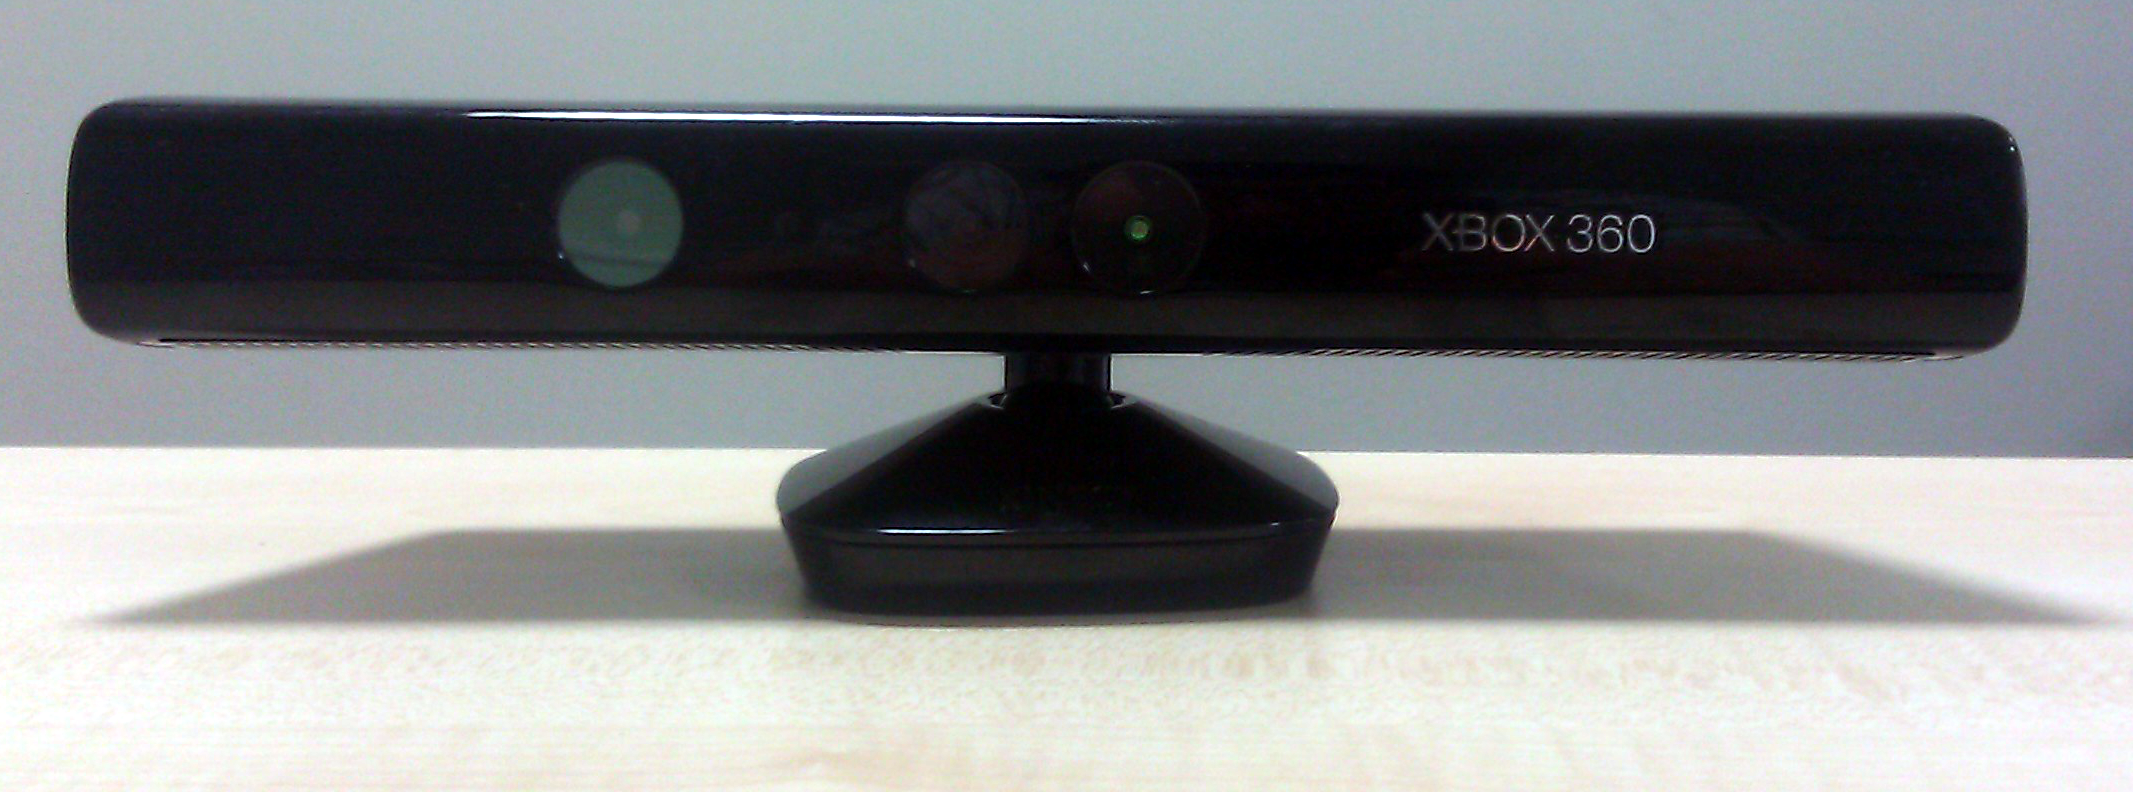
\includegraphics[width=0.45\textwidth]{figures/kinect.png}
   \caption{The Microsoft Kinect.}
   \label{fig:kinect}
\end{figure}

The firmware of devices which utilise light-coding offer several features relating to the tracking of a user.
These devices can outline any persons in front of the device and differentiate between them using their distances from the camera.
The device can then identify and give positional information on specific parts of a person's body, such as their limbs and joints if a calibration technique is executed.
This is usually a pose assumed by a person which allows the device to view a specific human outline from which it can identify joints and limbs~\cite{Xia2011}.
Using the difference between frames from the depth camera, the device's firmware can track the movement of people in its field of view.

The information a light-coding device can give concerning the positions of a person and their limbs offers a wealth of possibilities regarding computer interaction.
Specifically, the ability to obtain the positional information of people may be of use for co-located interfaces where interaction may require knowledge of the position of the user.
The ability to track and differentiate between users comes in useful for interaction technologies which allow users to share interfaces.
Dietz and Leigh~\cite{Dietz2001} note how the ability to track a user can be important.
Their research also identifies how existing techniques for tracking user positions which entail encumbering the user with extra devices are undesirable.
Light-coding devices offer the opportunity to track people without the need for users to wear additional devices.

Devices which can track the movement of user allow for movement about an environment without being constrained to an interface.
This is beneficial for teachers in classroom environment for whom mobility is vital.
There are alternatives to physical gesture sensing technologies which also afford this type of freedom from the interface.
Voice control is one such alternative where the teacher could issue commands to a technological framework in the classroom through a series of spoken instructions.
Using physical gestures alongside the voice commands could be beneficial as shown in the work of Bolt~\citeyearpar{Bolt1980}.
Allowing the user to gesture at where they want a specific command to influence reduces the need for additional spoken instructions.
However, the ambient noise in a typical classroom is likely to be too loud for voice recognition technologies~\cite{Cavalier1996,Goette1998,OHare1999}.
In addition to this caveat, the issuing of voice commands also will require teachers to interrupt their conversations with their students.

The use of physical gestures monitored via a light-coding device appears to be the most suitable approach to creating a system which allows teachers to control classroom technologies without the requirement for a distracting interface.

\section{Issues with Gesture-Driven Classroom Technology Orchestration} 
\label{sec:issues}

Light-coding devices could allow teachers to control technology in the classroom without the need for a physical interface.
Since physical gestures would permit eyes-free interaction~\cite{Brewster2003} with a control system, teachers could interact with students without losing control of the technology.
Due to a light-coding device's ability to track people in an environment, once a teacher is identified their movement around the classroom can be followed.
As a result of this, teachers could potentially issue commands through gestures from anywhere in the classroom.

Light-coding devices have high availability and relatively low cost in comparison to alternative depth sensing devices such as those used in Oblong's Mezzanine~\cite{kramer2011}.
Despite these potential benefits of light-coding device, there are several limitations that must be considered.
One limitation is their accuracy.
Light-coding devices are capable of tracking users and the position of their limbs.
However, for a light-coding device to track anything more precise, such as fingers, additional constraints on their abilities will need to be imposed \cite{Clark2011}.
These additional limitations potentially include a reduction in range, a reduced limit on the number of tracked users and the use of encumbering devices.
All these limitations are undesirable for the use of the device in the classroom.
Therefore, in the work discussed here, light-coding device will be assumed not be augmented to track anything more precise than user limbs.
This means that any gestures to be used by teachers for issuing control commands should consist of limb positioning and movement.

The inability of an un-augmented light-coding device to track anything more precise than user limbs discounts the adoption of gestures which use fingers for use in the classroom.
There are several reasons for gestures involving the use of the lower body limbs and joints, such as the legs, to be discounted also.
One such reason is their requirement for the visibility of the lower body.
In a classroom full of furniture and seated students, the teacher's lower body will potentially be obscured most of the time from the view of the light-coding device.
Due to these reasons, only gestures which utilise the positioning and movement of the upper-body should be considered when developing a classroom control system.
This means that gestures should only make use of upper-body joints and limbs which a light-coding device can track: the torso, wrists, hands, elbows, shoulders, neck and head.

\subsection{Considerations for Light-Coding in the Classroom}  
\label{subsec:considerations}

The use of physical gestures in the classroom requires that several considerations are taken into account in the design of any system which supports them.

\subsubsection{Avoiding False Positives}  
\label{subsubsec:falsePositives}

A potential issue concerning light-coding devices are that, by default, they are active at all times.
This means that teachers will need to be mindful of their actions.
Expressive body language or movement around the classroom could be interpreted by a light-coding device as a gesture.
This may trigger unwanted responses from any system utilising the device.
Therefore, a method of dismissing a light-coding device's attention and recapturing it later would be beneficial 
One potential solution to these false positives is to have designated areas from which gestures should be made.
This would allow teachers to move outside these areas without the possibility of accidentally issuing a command.
However, this solution does restrict the locations where the commands can be issues from, diminishing the ability of teachers to issue commands from anywhere.

A gesture based method of toggling a light-coding device's attention is another potential solution to the issue of a teacher unintentionally issuing commands through their movement in the classroom.
The light-coding device will not be able to issue any commands to a classroom technology unless its attention has been obtained by the teacher.
This results in the light-coding device used having two states: attentive and inattentive.
A gesture could be setup to be identified by the light-coding device in both states.
This gesture can be used to toggle state.
This diminishes the range of possible false gestures to one.
The solution reduces the chances of a teacher unintentionally issuing commands and allows for control over the light-coding device anywhere in the environment.
If this solution is adopted it is important to identify the gesture for gaining and dismissing the light-coding device's attention.

A potential drawback with the attention-toggling approach of managing these false positives is that if a teacher intentionally performs a gesture without getting the device's attention they will be ignored.
A false negative is preferable to a false positive because an unintended gesture may have irrecoverable consequences.
A false positive will have no consequence other than requiring the teacher to repeat their gesture again with the attention of the light-coding device.
Despite not being as problematic as the potential consequences of a false positive, the time-wasting result of a false negative is a potential issue.
A method of ensuring that a teacher knows whether they have the light-coding device's attention would be beneficial in stopping false negatives if the attention-toggling approach is taken.
Audible or visual feedback would aid the teacher in knowing whether their movement can or cannot be interpreted by the system as a gesture.

\subsubsection{Interface Selection}  
\label{subsubsec:interfaceSelection}

It is important to note that sometimes a teacher may wish to issue a command to specific selection of devices in the classroom rather than all.
This means that the teacher should be able to perform a gesture in such a way that the system is informed that the related action is intended to only affect specific devices.
A light-coding device's ability to track users can allow for the system to be informed of the location of a teacher in relation to the interfaces in the classroom.
Therefore, the teacher's proximity to interfaces could be used by a system to identify which devices a command should affect if informed of their locations.
However, the drawback to this approach is that if the teacher wishes to influence multiple interfaces they will be required to repeat the gesture in close proximity to each of the target interface which could take up an undesirable amount of time.
An alternative could be to use a specific gesture which can communicate a preferred device, or devices, to the system.
If implementing this into the design of a gesture set it is important to ensure this gesture is quick to perform and intuitive as it is likely to be repeated often by the teacher.


\section{Designing a Solution for Gesture-Driven Classroom Orchestration} 
\label{sec:solutionDesign}

% // TODO Some repetition in here so can be cut down.

With all the requirements for using gestures in the classroom and the limitations of the most suitable technologies outlined in Section~\ref{sec:issues} an important question becomes apparent:
\emph{Are gestures a viable method for controlling technology in the classroom?}

To answer this question a system for using gestures in the classroom first needs to be designed and implemented.
As part of the design a suitable set of gestures needs to be generated.
To inform the creation of the gesture set a focus group is utilised to find a set of relevant and un-intuitive gestures.
With a suitable set of gestures, a system which utilises them in the classroom can then be produced.
A study which utilises this system can then be used to answer the question of whether gestures are a suitable control technology for the classroom.

The requirements of the set of gestures to be used by teachers in the classroom are determined by both the shortcomings of the sensing technology, as discussed in Section~\ref{sec:issues}, and the abilities of the intended users.
Specifically, the set of gestures for controlling classroom technologies are those which are able to be detected by a light-coding device and are suited to be performed by teachers.
With the potential set of suitable gestures already reduced to the upper-body by the requirements of using the sensing technology in a classroom environment, there is now the task of identifying which gestures to use and with which controls.

\subsection{Gathering User Generated Gestures} 
\label{subsec:gatheringGestures}

It is important that the gestures selected for use in the study are intuitive~\cite{Cohen2002,Wachs2011} to allow teachers to easily remember gestures and perform them with minimal forethought.
Its also important that the number of gestures is kept small to avoid difficulties with requiring users to remember too much so that frustration with using the system can be minimised~\cite{Mendoza2005}.
The typical adult can remember seven items in a list, give or take two, in their short term memory~\cite{mil56}.
Relying on committing a greater number of commands to long term memory is undesirable since it counters the benefit that intuitive gestures offer of being quick to learn and use.

A framework for assessing potential gesture sets for the study must be decided upon.
An exhaustive literature survey utilising a structured protocol~\cite{kitchenham04} revealed that no framework currently exists for the evaluation of gestures meeting the requirements of classroom orchestration with upper-body gestures as outlined in Section~\ref{sec:issues}.
Therefore, an evaluation framework used for a similar set of gestures was required to be identified and adapted.

Nielsen et al.~\citeyearpar{Nielsen2004}'s work on procuring suitable sets of gestures for ergonomic interfaces entails the assessment of gestures using a framework of characteristics.
This framework is derived from a combination of usability principles and heuristics derived from ergonomic theory.
The characteristics the framework uses for assessment are a gesture's; (i) ease to perform and recall, (ii) intuitiveness, (iii) logical metaphoric and iconic links towards functionality and (iv) ergonomic nature.
Waches et al.~\citeyearpar{Wachs2011} outline a series of requirements which systems using hand-gestures should adhere to, a number of which echo the characteristics used in Nielsen et al.~\citeyearpar{Nielsen2004}'s work.
In addition to these are additional requirements which relate to the sensing technology used which relate to the technologies to be used in the study.

Because of their relevance it was decided that the requirements outlined by Waches et al.~\citeyearpar{Wachs2011} would be adopted for use to assess gestures in the study.
The more technical requirements and how a typical light-coding device adheres to them are as follows:

\begin{itemize}
\item  \textit{\textbf{Cost:}} As detailed in Section~\ref{sec:issues}, light-coding devices are relatively low cost.
\item \textit{\textbf{Responsiveness:}} The Kinect, a light-coding device, has a frame rate of 30Hz~\cite{Livingston2012} which is enough to be considered adequately responsive for tracking the movement of users.
\item \textit{\textbf{Adaptability:}} A typical light-coding device has the ability to be used by various supporting software frameworks which each allow accessing of the device's collected data and functions~\cite{Goth2011}.
This allows light-coding devices to be easily adapted for changes in use.
The scalability of a single light-coding device to track the joints and limbs of multiple persons is a demonstration of its ability to adapt to different numbers of users.
\item \textit{\textbf{Accuracy:}} The Kinect, a light-coding device, is noted to track user's limb and joints to 20mm when in range~\cite{Marquardt2011}.
\item \textit{\textbf{Un-encumbering nature:}} When a user is required to wear a device for some purpose, the affiliated system is considered to be encumbering.
This can be undesirable as it detracts from a system's ubiquity and may impede use. 
Since a light-coding device can track users through a single static device which does not need to be worn it is considered to be un-encumbering.\\ 
\end{itemize}

One of Waches et al.'s~\citeyearpar{Wachs2011} requirements refers to the gesture set itself.
A criterion based on this requirement can be stated as follows:

\begin{itemize}
\item \textit{\textbf{Lexicon Size:}} The size of the gesture set must not be too large.
This criterion can be adhered to by taking into account the limitations of short term memory.\\ 
\end{itemize}

The remainder of the requirements outlined by Waches et al.~\citeyearpar{Wachs2011} refer to requisites of the hand gestures themselves.
A summary of these criteria for upper-body gestures based on these requirements can be outlined as follows:

\begin{itemize}
\item \textit{\textbf{Intuitiveness:}} A gesture which a user performs naturally in relation to a specific command action is beneficial.
\item \textit{\textbf{Comfort:}} If a gesture is uncomfortable to perform a user is unlikely to perform it frequently, thus diminishing the benefit of the system.
\item \textit{\textbf{Low mental load:}} For a gesture to conform to this criterion a user should be able to perform it with little forethought.
\item \textit{\textbf{Interaction space:}} Gestures which require large amounts of space to be performed limit the locations it can be performed.
Therefore, to fulfil this requirement, gestures should minimise used space.
\item \textit{\textbf{Ubiquity:}} A gesture which does not appear to be in keeping with a user's typical actions in the current environment would not fulfil this criterion. \\ 
\end{itemize}

Using these criteria, any suggested gesture sets and their suitability can be assessed to be viable or not.

\subsection{Focus Group} 
\label{subsec:focusGroupDesign}

To discover gestures which conform to the criteria outlined in Section~\ref{subsec:gatheringGestures} a user-centred design process was adopted.
As part of this process a user study in the form of a focus group was organised.
Through the focus group a user-generated set of viable upper-body gestures for use with a light-coding device was discovered.
The focus groups acted as a form of guessability study~\cite{Ruiz2011,Wobbrock2009} which would generate gestures which are natural to the user~\cite{Grandhi2011}.
User-generated gestures for surface computing are noted to be intuitive, comfortable, memorable and ubiquitous~\cite{Bjorneseth2012}.
These potential benefits of user-generated gestures adhere to the criteria relating to the definition of effective upper-body gestures.

The primary objective of this study was to find the quickest, most intuitive and least intrusive upper-body gestures which can be performed in the classroom to execute the most important control commands.

Three focus group sessions took place.
All participants were required to have had some experience of teaching in a classroom environment.
Participants were asked to position themselves in the room used in the study facing away from each other and towards the cameras recording the session to reduce the influence that they would have on each other.
In each session a number of the participants were asked to stand and the rest were seated.
A list of commands that teachers using a classroom control system may need to issue was compiled.
The commands used were those for: 
\begin{itemize}
\item Freezing/Unfreezing student interfaces.
\item Sending contents of student interfaces to a shared interface.
\item Sending contents of a board interface to student interfaces.
\item Showing snapshots on the board interface of the student interfaces.
\item Clearing the student interfaces.\\
\end{itemize}

These commands were decided upon based on observations on which were the most frequently issued during previous studies~\cite{Hatch2011}.
It was decided to adhere the lower bound of short term memory, discussed in Section~\ref{subsec:gatheringGestures}, of five.
This relatively small gesture set conforms to the Wachs et al.'s~\citeyearpar{Wachs2011} requirement for a small lexicon size.

For each command participants were asked to perform the first gesture that they thought of which related to it meaning  that the gestures performed were likely to be natural to the participant.This is beneficial for finding gestures which conform to the criteria outlined in Section~\ref{subsec:gatheringGestures}.
Spontaneous and frequently repeated gestures are assumed to be natural to the user and therefore are \textit{\textbf{intuitive}}~\cite{Grandhi2011}.
The intuitive nature of the gestures also implies that they are \textit{\textbf{comfortable}} for participants to perform.
Since participants were asked to put little thought into their motions, the gestures can also be said to have a \textit{\textbf{low mental load}}.
Participants were placed closely side-by-side helping ensure that the gestures used would utilise a restrained \textit{\textbf{interaction space}}.
Participants were also asked to be mindful of the fact that these gestures would be performed in a classroom environment to ensure that the gestures suggested by participants would be in some part \textit{\textbf{ubiquitous}} to the classroom environment.

Participants in the study were asked to perform two gestures for each command.
The first gesture related to a command issued to all interfaces whereas the second related to a command intended for a specific selection of interfaces.
Participants were made aware that gestures should only use the upper-body but not fingers and that a gesture can either be a pose or movement.
Participants were also informed that they could not assume their promiximity to a device could not be used for selecting a specific interface.

\subsubsection{Focus Group Data Analysis}
\label{subsubsec:focusGroupDataAnalysis}

Using video recordings of the focus group sessions all participants' movements for each command could be studied and summarised as a sequence of poses and movements.
This allowed the participants' actions to be formalised as gestures.
These gestures could then be compared, allowing similar actions to be identified as being separate instances of the same gesture.
The gestures which were used most frequently for specific commands could then be identified.
The most frequently occurring gesture for a command is likely to be the most intuitive since they will match the intended users' mental model of how the system should be used~\cite{Nielsen2004,Ruiz2011,Wobbrock2009}.

Each unique gesture identified was first evaluated against the limitations of a typical light-coding device.
Any gestures which did not conform to these limitations, such as those which used finger motions, were discounted.
Following this, the criteria outlined in Section~\ref{subsec:gatheringGestures} were used to assess the gestures.
Any gesture which did not meet the criteria was also discounted.
The viable gestures observed for a command across all the sessions were then ranked by frequency to identify those to be considered most intuitive.

If more than one command had the same gesture with the highest frequency, the gesture would be assigned to the command with the highest usage observed in past studies~\cite{HatchA.HigginsSMercier2009}.
The less used commands would then be assigned their gesture with the next highest frequency.

It was decided that the attention toggling method of managing false positives, discussed in Section~\ref{subsubsec:falsePositives}, would be adopted due to its ability to reduce errors without placing constraints on where in an environment gestures can be performed.
Every effort was made to ensure participants' minds were kept clear of any assumptions about the system to aid the performance of intuitive gestures~\cite{Nielsen2004}.
As part of this effort it was decided that the participants should not be made aware of the toggle mechanic.
Since this gesture potentially needs to be performed prior to any other command gesture, it will be the most frequently used in the system.
Therefore, the most frequently occurring gesture throughout the entire study was chosen for this mechanic to ensure that is is intuitive and natural.

The data analysis also aimed to identify how the participants differentiated gestures intended for all interfaces from those intended for specific interfaces.

\subsection{Focus Group Results}
\label{subsec:focusGroupResults}

Of the sixty seven participants who took part in the study, fifteen were male and fifty two were female.
This was representative of the gender balance of \ac{PGCE} students at the institution.
The majority of these participants were aged between twenty and twenty five.
The video recordings from the study were analysed by the first author.
From the analysis of the videos, several patterns in the participants' gestures were observed.

\subsubsection{Toggling Attention}
\label{subsubsec:focusGroupResultsTogglingAttention}

The most common gesture was a simple horizontal wave of a single hand.
Seven percent of all gestures observed in the study comprised of the waving of a single hand.
This was used by participants frequently and may have been a gesture for actions where the participant could not think of an appropriate gesture. 
While some participants would not perform a gesture for commands that they could not think of a suitable gesture for, others would instead perform a generic gesture, referred to as a \textit{default gesture}.
This set of default gestures were not specific to any particular subset of commands but were frequently used by participants.
In addition to waving with one hand these default gestures included; holding one hand up and pointing with one hand.
These gestures accounted for twenty eight percent of the observed gestures in the study.

\subsubsection{Interface Selection}
\label{subsubsec:focusGroupResultsInterfaceSelection}

7\% of the study's participants showed no clear method of differentiating between commands that affect all interfaces or those which affect specific interfaces. 
These participants would either repeat the same gesture for both instances of the command or would have no single consistent differentiation approach for the commands. 

To differentiate between commands which affect all interfaces and those which affect specific interfaces, 93\% of the participants would always follow a consistent approach.

\begin{itemize}

\item \textbf{Use two completely different gestures.}\\
A minority, 23\% of participants, would always perform different gestures as a method of differentiating a command applied to either all or specific interfaces.
This differed from the majority who would use the same gesture for a command when applied to all or specific interfaces with a slight deviation between them.
A drawback with the approach of using different gestures is that it effectively doubles the number of gestures a teacher must remember since each command would have two gestures affiliated with it.
This would increase the number of gestures to ten which is unacceptable since it may to be large for many potential users' short-term memory.
Another drawback to this approach was that the gesture intended to affect specific interfaces would be required to utilise the light-coding device's user tracking ability to determine which interface the teacher is closest to.
This would require the teacher to repeat the gesture for all interfaces they wish to the command to be applied to making the issuing of commands take significantly longer.

\item \textbf{Use different sized versions of the same gesture.}\\
5\% of participants were noted to perform the same gesture for issuing a command but would differentiate between whether it would affect all or a specific subset of interfaces through the size of the gesture.
The size of the gesture is defined by the amount of space that it occupies.
For example, some gestures involved the user drawing a circle with their hands.
For what would be considered a small gesture for some participants, this circle would have a diameter under half a metre.
For these participants a large version of the gesture would entail the user drawing a circle with a diameter larger than half a metre.
For all participants using this approach, the small version of a gesture was applied to the command affecting only specific interfaces.
For this approach to be implemented, the small gesture would have to use the teacher's proximity to the interfaces to determine which to affect.

\item \textbf{Perform the gesture with either one or two hands.}\\
Another approach adopted by participants for differentiating between a command that affects all interfaces or specific interfaces was defined by the number of hands used. 
The 8\% of participants who followed this approach constantly throughout the study would all use a single hand to perform gestures intended to affect specific interfaces.
These participants would then perform the same gesture with both hands when applying the command to all interfaces.
This approach, like that which utilises the size of the gesture, requires teachers to repeat the one-handed version of a gesture in close proximity to all the interfaces they wish to affect.

\item \textbf{Perform the gesture and pointing at the interfaces it should affect.}\\
The majority of participants, 57\% in total, would perform a pointing gesture to signify a command affecting specific interfaces.
This pointing gesture would be where participants locked their arm in a straight line.
Some of the participants performing this gesture would also point with a finger but this would be ignored by a sensing technology as inaccurate as a light-coding device.
Participants who adopted the approach of pointing at the interfaces they wished to affect would perform the command gesture on its own when wishing to issue the command to all interfaces.
This was the most popular method of differentiating between whether a command should affect all or specific interfaces.
3\% of participants who adopted the pointing approach would always perform the gesture with one hand and point with the other throughout.
Alternatively, participants would perform the command and pointing gestures sequentially.
All of these participants would point first and then perform the gesture.

\end{itemize}

\subsubsection{Command Gestures}
\label{subsubsec:focusGroupResultsCommandGestures}

Noted in the analysis was that despite many of the gestures being one handed, participants did not use handedness to distinguish between single hand gestures for various commands.
Participants may have considered that a gesture which is required to be used with a specific hand may be problematic for those whose handedness differs from their own.
This implies that hand-dominance did not influence which gestures participants considered for the commands.

\begin{figure*}[p]
   \centering
   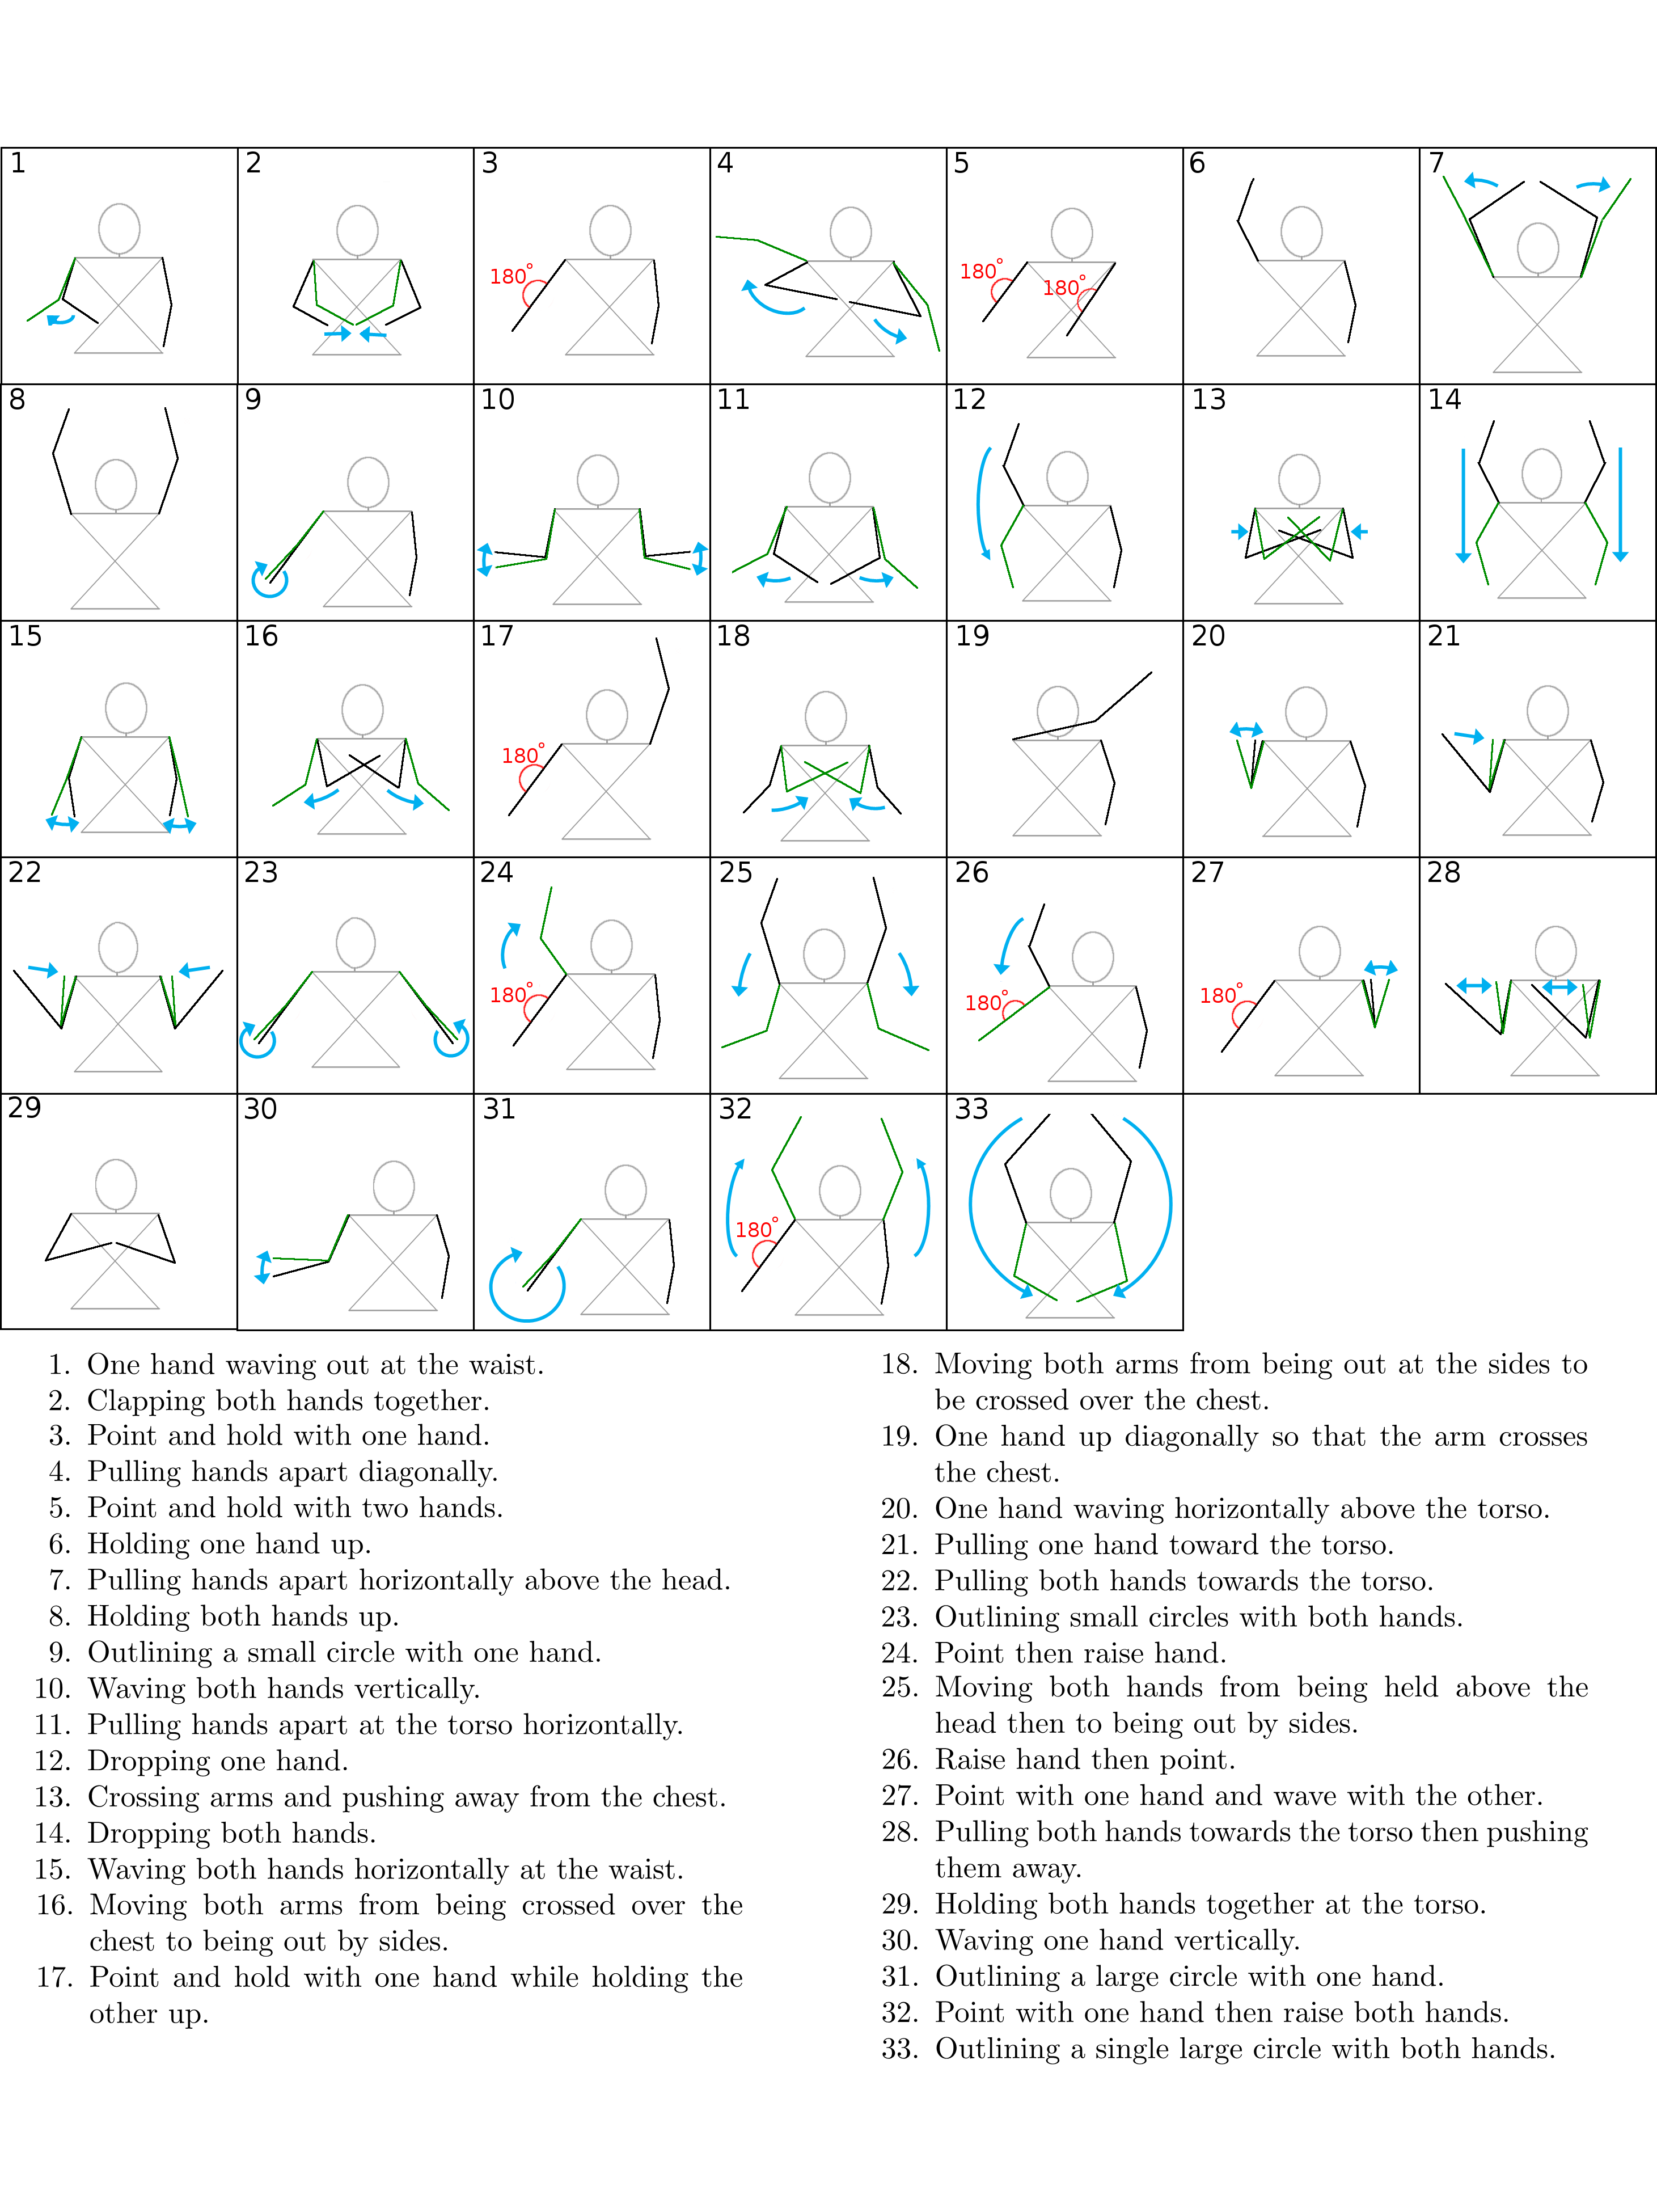
\includegraphics[width=1\textwidth]{figures/all_gestures.png}
   \caption{All unique gestures observed during the study.}
   \label{fig:allGestures}
\end{figure*}

Thirty three unique gestures which conform to the criteria outlined in Section~\ref{subsec:gatheringGestures} were observed during the study.
These gestures are shown and described in Figure~\ref{fig:allGestures}.  

After reviewing the videos and attaining the number of occurrences for each gesture per command over all the studies, the most frequently used gestures for each command could be identified.
Popularity refers to the gestures frequency of occurrences and was used as it often indicates intuitiveness~\cite{Grandhi2011}.
The results are as follows: \\

\begin{itemize}

\item \textbf{Freezing/Unfreezing the classroom interfaces.}\\
\textit{Gesture 8: Holding both hands up.}\\  
10.65\% of the gestures performed for this command exclusively entailed participants holding both hands up.
The popularity of this gesture for the freeze command is likely due to its similarity with the commonly used halt or stop hand signal.\\

\item \textbf{Sending contents of the classroom interfaces to the board.}\\
\textit{Gesture 6: Holding one hand up.}\\
1.12\% of the gestures performed for this command exclusively entailed participants holding a single hand up.
There were so many unique gestures performed for this command that even the more popular gestures had only a small share of the total.
Though holding a single hand up was popular amongst many of the participants for a variety of commands, it proved to be most popular for sending contents to the board.\\

\item \textbf{Sending contents of the board to the classroom interfaces.}\\
\textit{Gesture 21: Pulling one hand towards the torso.}\\
15.49\% of the gestures performed for this command exclusively entailed participants pulling a single hand towards their torso.
This gesture was likely popular because the motion gives the appearance of the teacher beckoning content from the board, effectively pulling it towards the classroom interfaces.\\

\item \textbf{Showing snapshots on the board of the classroom interfaces.}\\
\textit{Gesture 29: Holding both hands together at the torso.}\\
10.26\% of the gestures performed for this command exclusively entailed participants holding both their hands together near their torso.
Many participants made a gesture with their fingers for this command emulating taking a photo on a camera.
When asked to modify their behaviour so that they did not use their fingers (due to the limitations of light-coding devices discussed in Section~\ref{sec:issues}) participants often performed Gesture 21 instead.
This gesture is as close to emulating taking photos as possible without the use of fingers.\\

\item \textbf{Clearing the classroom interfaces.}\\
\textit{Gesture 11: Pulling hands apart at the torso horizontally.}\\
48\% of the gestures performed for this command exclusively entailed participants pulling both their hands apart near their torso.
This gesture was likely popular due to its similarity to the real life action of sweeping objects off a surface.
The second most popular gesture for this command was gesture 15, waving both hands horizontally at the waist.
Again, this gesture was likely to be popular due to its similarity to the action of clearing objects off a surface.\\

\end{itemize}

With this set of gestures compiled, a gesture recognition system can be implemented into a classroom technology system utilising a light-coding device.

\subsection{User Generated Gestures}
\label{subsec:userGeneratedGestures}

The results from the focus group discussed in Section~\ref{subsec:focusGroupResults} indicated that the gestures which were the most popular were those that bore a metaphorical relationship to their corresponding commands.
If a command could be interpreted as a physical task, participants would often use a gesture which mimicked an action carried out to complete that task.
This re-iterates the importance of metaphor when designing intuitive systems \cite{Wang2008}.
All of the metaphoric gestures observed in the study were pantomimic, where the user mimics a related real-world action.
As shown in the work of Grandhi et al. \citeyearpar{Grandhi2011}, gestures which are pantomimic have a greater chance of being intuitive.
In addition to being a familiar and natural action, a metaphor-based gesture is easier for a user to remember due to its connection to the task it represents.
Of the five gestures chosen for the commands, four could be interpreted as being metaphor-based.
Only gesture 6, the holding up of one hand to send content to the board does not directly represent a related action.
This may be because any physical actions related to this task are not as obvious as the actions which other gestures emulate.

As discussed in Section~\ref{subsec:gatheringGestures}, criteria derived from the requirements outlined by Wachs et al.~\citeyearpar{Wachs2011} relating to the sensing technology are fulfilled by the proposed use of a light-coding device.
Using the results of the focus group based study; this set of five command gestures can be used to control some systems of classroom technology that entail the sharing of content between teacher and student interfaces.
In addition to this, gesture 20; the horizontal wave above the torso, is suitable for obtaining and dismissing the light-coding device's attention.

The pointing approach discussed in Section~\ref{subsec:focusGroupResults} was the most popular option for use when defining which interfaces a command affects.
The alternative approaches require the teacher's proximity to interfaces.
This entails teachers moving about the classroom to perform gestures which would be time consuming and disrupt interaction with the students.
There are also other issues with the alternative approaches.
For example, the approach which uses the size of the gesture to determine whether it affects all or just the nearest interface is subject to a teacher's interpretation of what constitutes a large gesture.
The \lq small\rq\ gesture of some participants was larger than the \lq large\rq\ gesture of others.

A control sequence that uses the proposed set of gestures should utilise pointing for table selection based on the popularity of this approach in the focus group.
The sequential approach of pointing then gesturing allows for multiple interfaces to be selected before executing a command, something other approaches of selecting interfaces would not allow for.
This saves time because the teacher would not need to repeat the gesture.

\begin{figure*}[t]
   \centering
   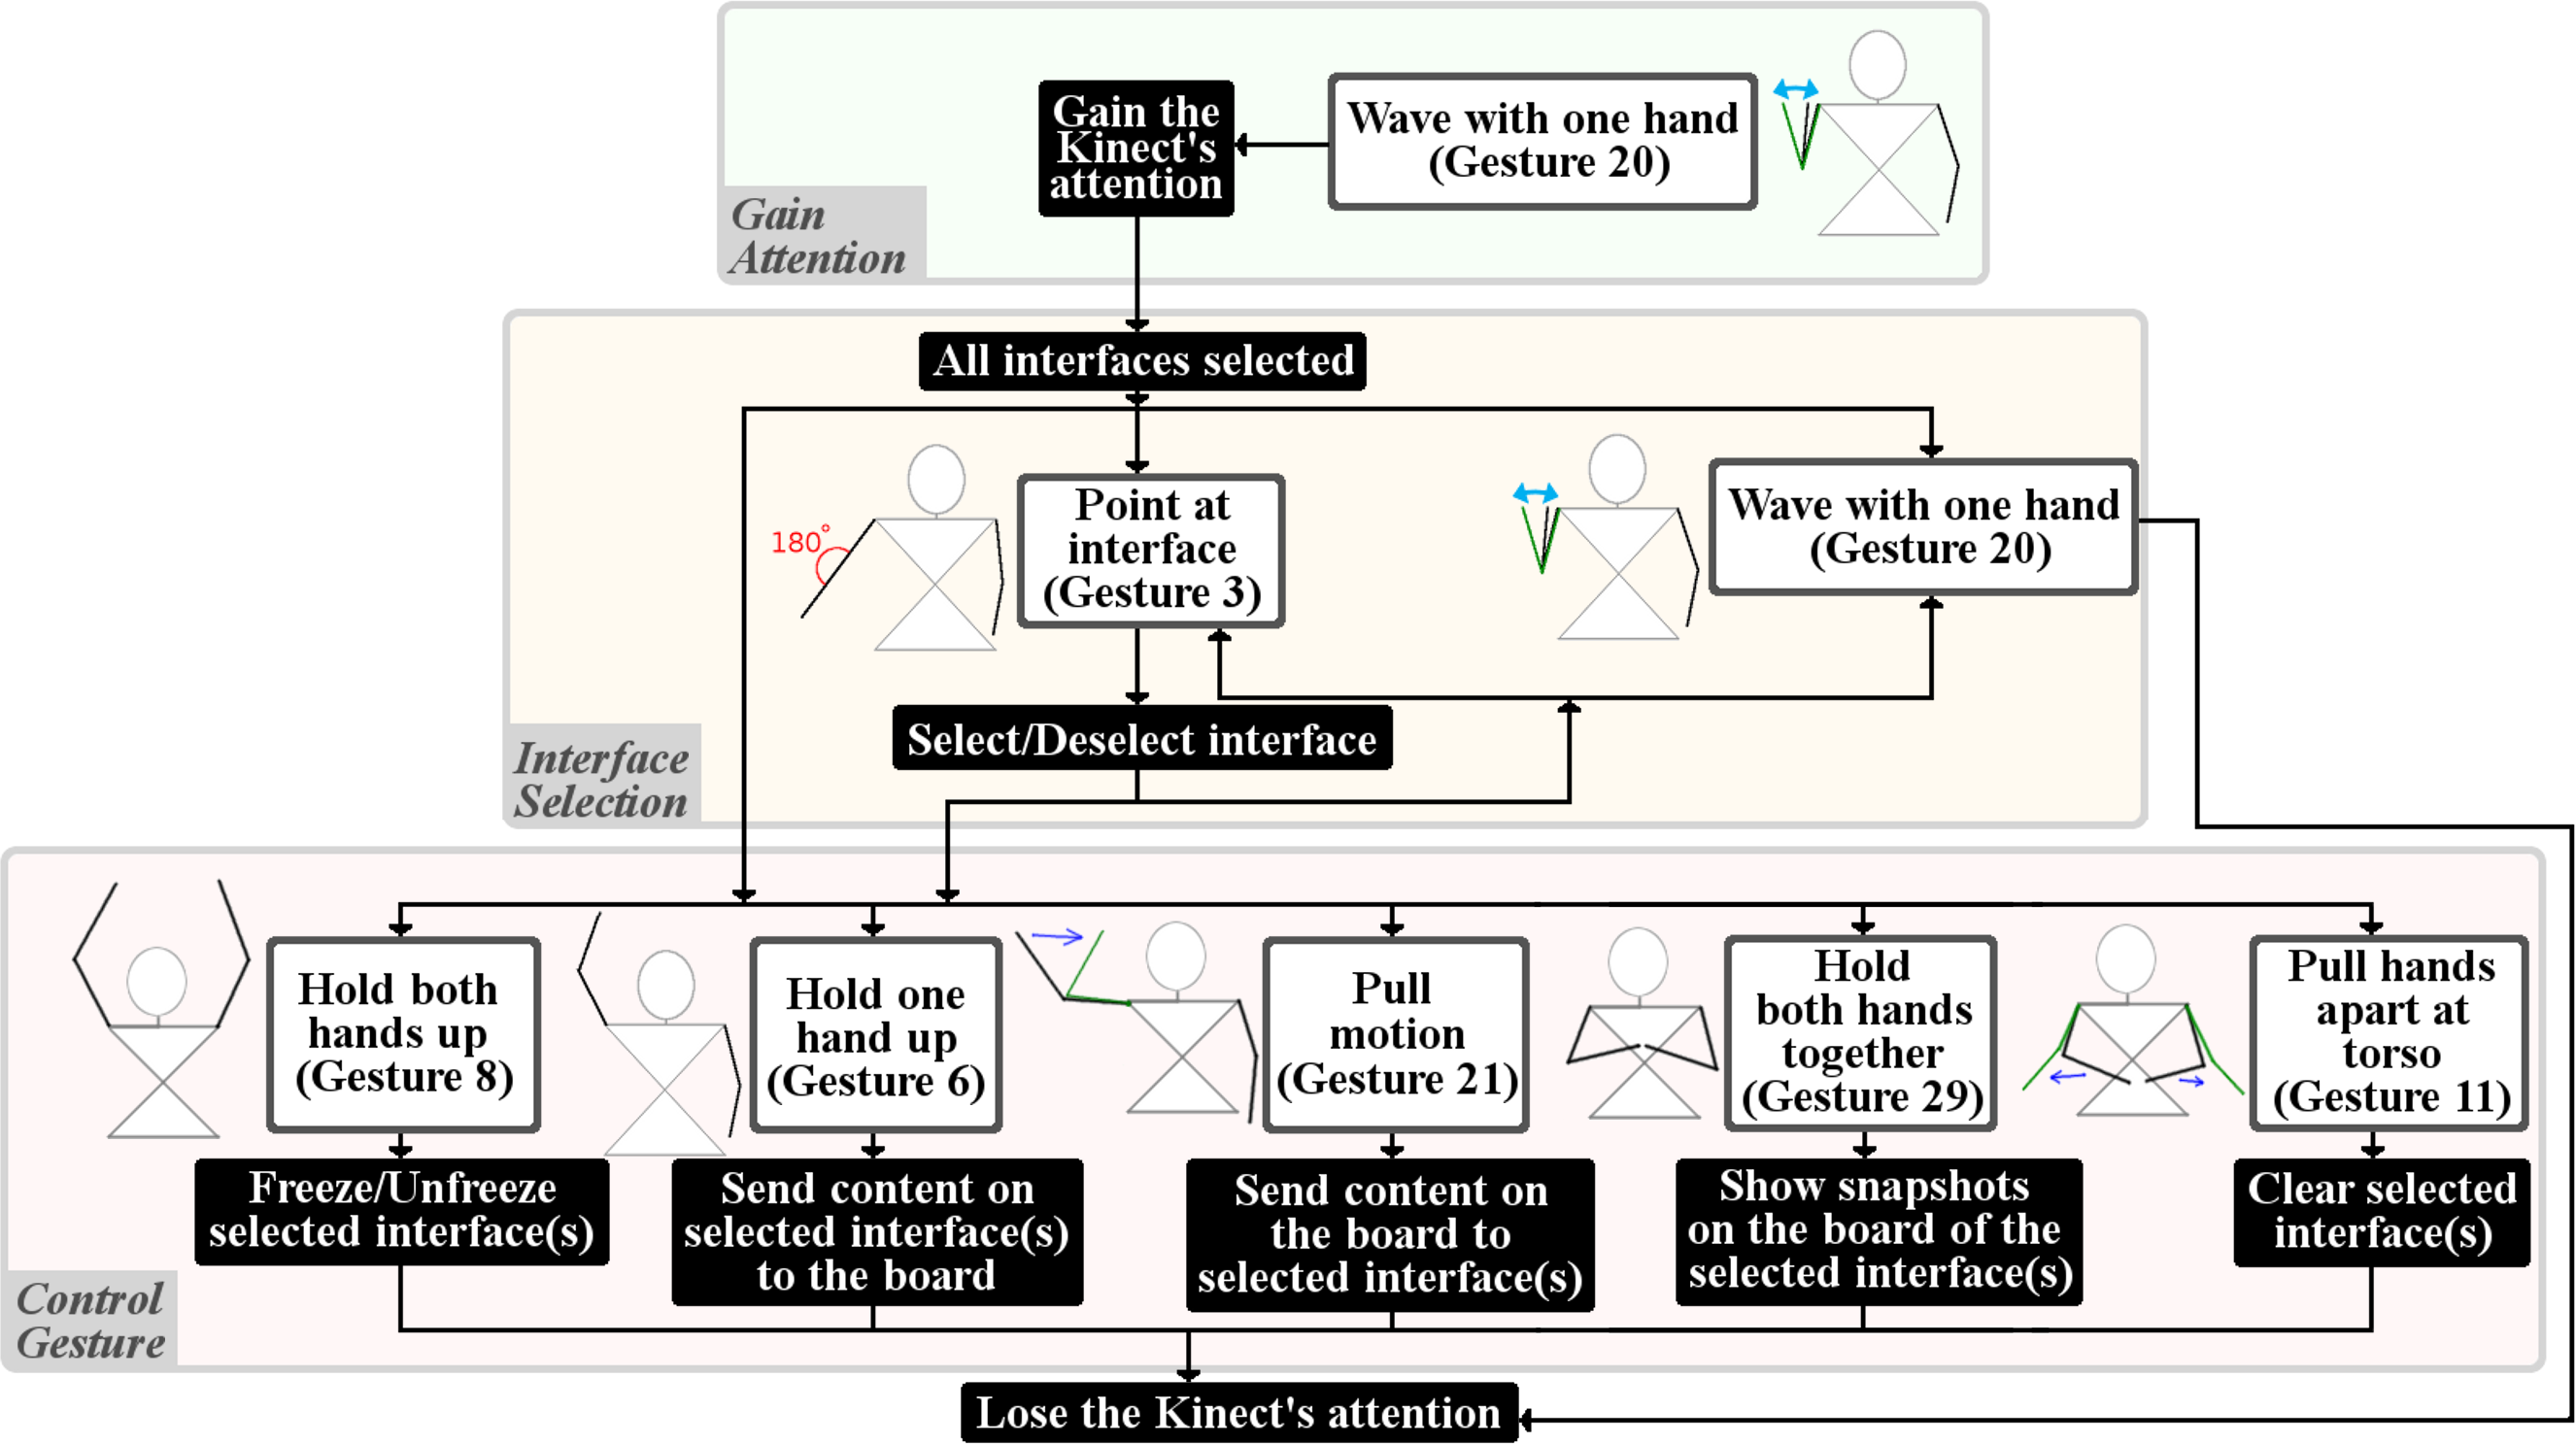
\includegraphics[width=1\textwidth]{figures/control_flow.png}
   \caption{How the gesture identified in the focus group are intended to be used.}
   \label{fig:flow}
\end{figure*}

Figure~\ref{fig:flow} outlines a control sequence in which the gestures and approaches to interface selection indicated by the focus group to be intuitive can be used to issue common commands to classroom technologies.
Teachers first obtain the light-coding device's attention with a wave then point to the interfaces they wish the following command gesture to affect.
The teacher can repeatedly point to interfaces to select and deselect them until they perform the command gesture.
Alternatively, the teacher can perform the command gesture immediately after obtaining the light-coding device's attention to issue the corresponding command to all interfaces.
At any time during this control sequence a teacher can wave again to dismiss the light-coding device's attention.
After the command gesture is performed the light-coding device stops paying attention to the teacher.

For each response of the system to teacher gestures, denoted in Figure~\ref{fig:flow} with the black boxes with white text, some form of feedback will need to be provided to the teacher.
This feedback is necessary for informing the teacher whether the gesture they have performed has had the intended effect on the system or not.

With the gesture set and control sequence defined, a classroom technology system can be augmented to use a light-coding device.

\section{Pilot Study}
\label{sec:pilotStudy}

To explore the suitability of the defined gesture set to use with a light-coding device it was decided that a pilot study was needed.
This pilot study would allow for any short-comings in the technology or gesture-set to be identified and corrected before carrying out any further studies.

\subsection{Software Implementation}
\label{subsec:pilotStudyImplementation}

The SynergyNet framework~\cite{Higgins2011} was selected for implementing the control sequence defined in Section~\ref{sec:background} into.
SynergyNet is a software framework which supports education based activities that are intended to be interacted with through multi-touch table interfaces.
The framework offers a wide range of supporting features such as communication between multiple interfaces via a network and is capable of displaying several forms of media.
SynergyNet accepts inputs from a range of multi-touch protocols, such as TUIO~\cite{Kaltenbrunner2009}.
Though initially intended for use with diffused illumination multi-touch technology~\cite{Matsushita1997}, the support of multiple protocols allows the framework to be used with a wide range of natural user input interfaces including interactive whiteboards and multi-touch tables.

Applications for SynergyNet often utilise the network functionality of the framework to allow teachers to orchestrate classroom activities.
Previously, teachers have been able to do this through a static multi-touch device~\cite{AlAgha2010}.
Teachers can also orchestrate SynergyNet through a web interface which can be accessed through a mobile touch device, such as a phone or tablet~\cite{Mercier2013}.
In previous studies using the SynergyNet framework it was noted that the use of both the static teacher console and mobile devices to issue commands distracted the teacher from the students whenever used~\cite{Hatch2011,Mercier2013}.
This often disrupted conversations between the teacher and students.

The SynergyNet framework may benefit greatly from the use of upper-body gestures. 
The commands chosen to find gestures for in the study were based on those used in the existing SynergyNet controls. 
Several commands facilitated by these controls involve sharing materials between student interfaces and the classroom's board; a large, wall mounted interface used to display content to a class.
These commands have been observed in previous studies of SynergyNet to be essential for orchestrating tasks across the system.

To support the implementation of the gesture control sequence a light-coding device was required.
The Microsoft Kinect was chosen due to its low cost and availability.

\begin{figure}[h]
   \centering
   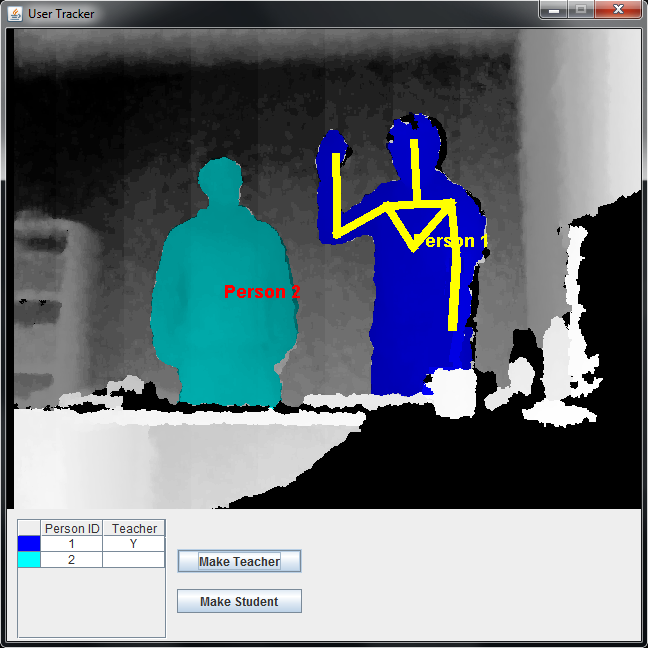
\includegraphics[width=0.45\textwidth]{figures/kinect_node.png}
   \caption{SynergyNet's Kinect node.}
   \label{fig:kinectNode}
\end{figure}

To integrate the Kinect with SynergyNet, the SensorKinect driver~\cite{Avin2011}, OpenNI library and NITE framework~\cite{Organisation2011} were used together~\cite{Davison2012}.
Instances of SynergyNet running on the same network act as nodes which communicate through Hazelcast~\cite{Hazelcast2009}.
There are several different types of node used by SynergyNet defined by what device they as used on such as student-centric touch-screens or teacher control consoles.
For the implementation of the Kinect a new type of node was created which would manage tracking users, identifing gestures and displaying its current output, as shown in Figure~\ref{fig:kinectNode}.

The Kinect node obtains information on user locations relative to the sensor device position direct from the OpenNI framework.
Prior to use all SynergyNet nodes, including the Kinect node, will be configured so that it knows its associated device's position and orientation in the environment.
Before transmitting a tracked user's locational information, the Kinect node will use the knowledge of the sensing device's position to transform the locational information regarding the user to derive positions relative to the environment.

The Kinect node is used to identify when specific gestures are performed by a teacher.
When a teacher is observed performing a gesture the corresponding command is sent through the network to the relevant SynergyNet nodes.
The Kinect node has on-screen controls which allow identified persons to be designated as students or teachers, as shown in Figure~\ref{fig:kinectNode}.

Support for multiple Kinect devices was not possible in this pilot due to issues surrounding how the device's depth-detection techniques would interfere with other Kinect devices nearby.
This meant that the use of the pointing gesture outlined in Section~\ref{subsec:userGeneratedGestures}'s defined control sequence used for selecting interfaces could not be implemented into SynergyNet.
For the pilot study it was decided that any commands issued through gestures would have to affect all student interfaces.

To minimise the potential of a false positive, a timer was implemented into the control sequence which would dismiss the Kinect's attention if no valid gestures are detected.
Once a teacher has waved and gained the attention of the Kinect they would have thirty seconds to perform a gesture in the control sequence.
Otherwise, the control sequence ends and the Kinect's attention is dismissed.
This ensured that if a teacher unknowingly gains the attention of the Kinect, the amount of time they could perform a gesture accidentally in is limited.

As discussed in Section~\ref{subsec:userGeneratedGestures}, the system needs to provide feedback to the teacher for each action of the system denoted in Figure~\ref{fig:flow}.
As part of the control sequence a sound was played when the Kinect's attention is gained to alert teachers of successful intentional or accidental unintentional waving gestures.
The use of audible feedback allows the teacher to be informed of this event without the need to focus on a visual output.
A visual form of feedback was also offered due to the potential problem of audio with ambient classroom noise as discussed in Section~\ref{sec:background}.
This visual feedback took the form of a border appearing on the Kinect node display.
A border also appears on all the student interfaces at this stage to indicate they are awaiting a command gesture.
This increases the chance of the teacher seeing the feedback informing them that they have successfully gained the Kinect's attention.

For the actions resulting directly from a command gesture the teacher can visually see the effect of the completed action as a form of feedback.
The movement and removal of content is clear enough that no additional feedback is required.
For the freezing and unfreezing of the system a blue tint is applied to the student interfaces in adherence to the metaphor of its content being frozen.

When the control sequence is finished the borders are removed from the Kinect node and student interface to indicate that the system's attention is lost.

\subsection{Pilot Study Design}
\label{subsec:pilotStudyDesign}

% // TODO Trim down and make appropriate to section - focus on just the kinect.

A user study was conducted as an observed lab-based experiment.
The study took place in the SynergyNet lab used in the focus group discussed in Section~\ref{subsec:focusGroupDesign}.
In this study the upper-body gesture driven Kinect device was compared against two existing control devices used by SynergyNet in previous studies~\cite{Mercier2012}.
This would allow for the suitability of the gestures derived from the focus group and their encompassing control sequence's implementation into SynergyNet to be assessed.

\begin{figure}[h]
	\centering
	\begin{subfigure}[h]{0.23\textwidth}
		\centering
		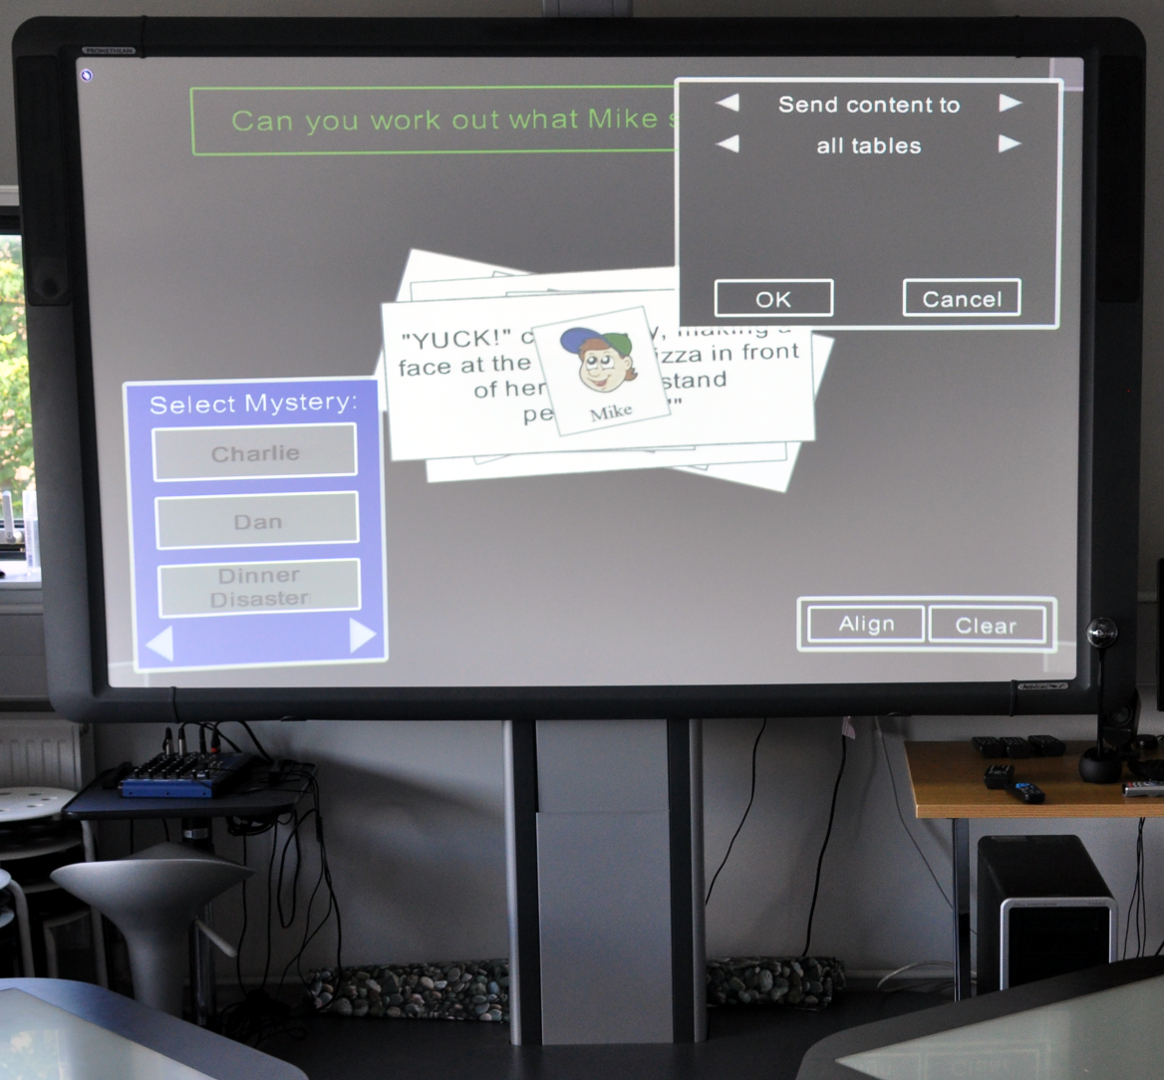
\includegraphics[width=\textwidth]{figures/control_board.png}
		\caption{The multi-touch board showing teacher controls.}
		\label{fig:controlBoard}
	\end{subfigure}
	\begin{subfigure}[h]{0.23\textwidth}
		\centering
		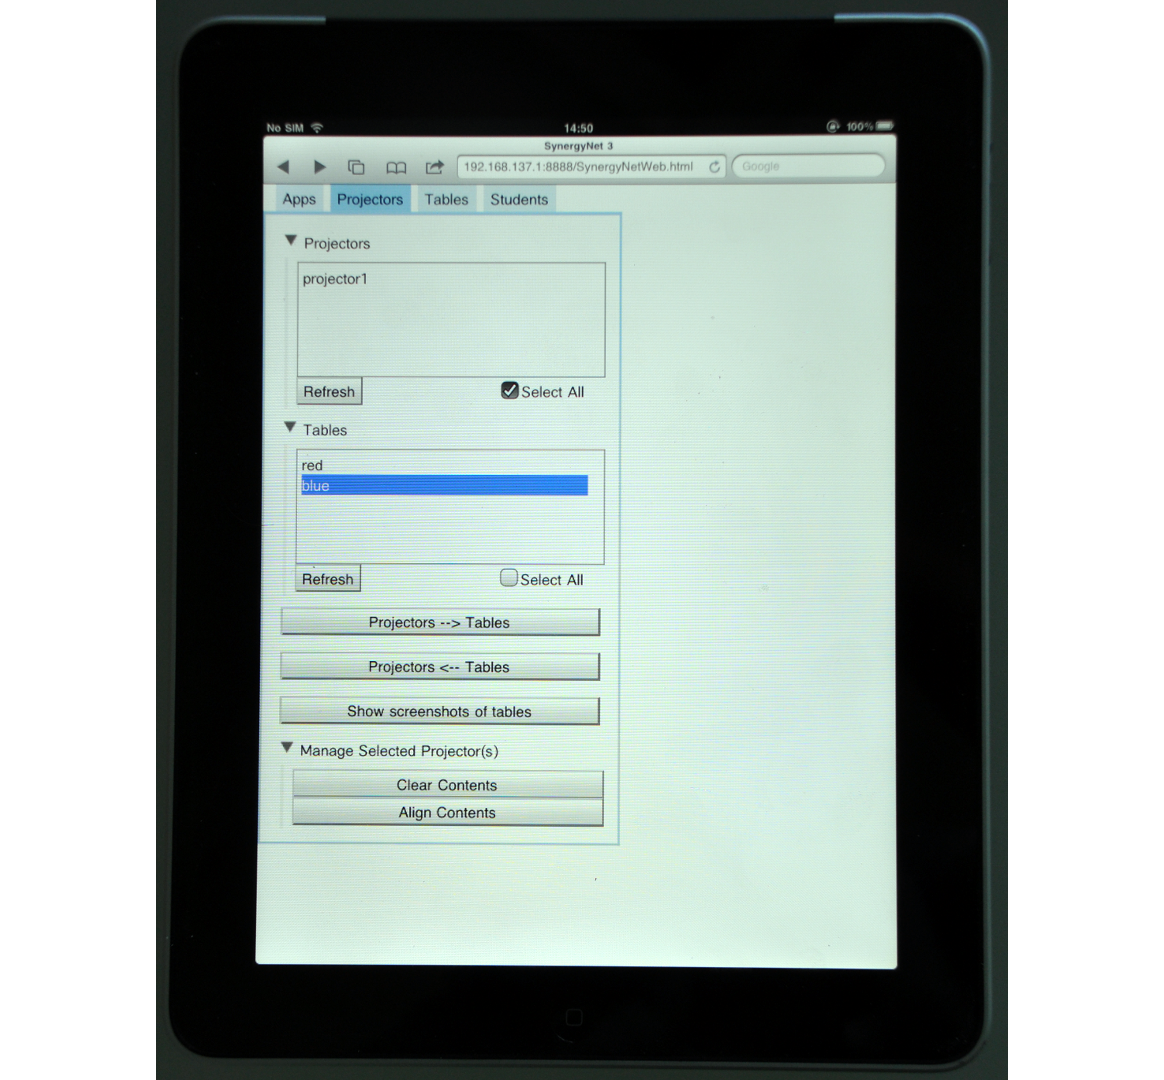
\includegraphics[width=\textwidth]{figures/control_tablet.png}
		\caption{The web interface via an iPad tablet.}
		\label{fig:controlTablet}
	\end{subfigure}
   	\caption{The interfaces used to control SynergyNet.}
   	\label{fig:controlDevices}
\end{figure} 

Prior to the incorporation of the Kinect, SynergyNet supported two control technologies which teachers could use to control instances of the framework on student-centric multi-touch interfaces as discussed in Section~\ref{sec:background}.
In the lab, a multi-touch interface for the teacher controls, used to issue the commands listed in Section~\ref{subsec:userGeneratedGestures}, has been made available through an interactive whiteboard shown in Figure~\ref{fig:controlBoard}.

As an alternative to the multi-touch based controls, teachers can also orchestrate instance of SynergyNet through a web interface.
This web-based control interface is made accessible in the lab through an iPad tablet device as shown in Figure~\ref{fig:controlTablet}.

The primary objective of this study was to find how the upper-body gestures compare to the alternative control technologies.
The hypothesis was that the gestures would allow commands to be issued quicker and with fewer errors due to their intuitiveness.

The head teacher from a local school was chosen for participation in this study through convenience sampling.
A class of 12 of teacher's students who the teacher had taught previously also participated.
This class consisted of eight girls and four boys aged eight to ten.
The participating teacher was first given an hour long training session where they were brought into the SynergyNet system and lab.  
In this session, the teacher gained experience in using the three control technologies.

Following the training session, the teacher's class of students were introduced to the classroom.
The students were given the chance to gain familiarity with the multi-touch tables through interacting with several simple SynergyNet applications.
Following this the class then started the first \textit{mysteries} task.
Mysteries are a pedagogic technique, designed to support collaborative problem solving~\cite{Leat2002}.
The mysteries task gives groups of students a selection of clues relating to a particular scenario~\cite{Higgins2011b}.
Students are then given a question which they must use the clues to answer.
The task was chosen due to its requirement for the teacher to perform all the commands outlined in Section~\ref{subsec:userGeneratedGestures} throughout~\cite{Mercier2012}.
During the first task the teacher only had access to the multi-touch board for controlling the student-centric interfaces.

A second mysteries task began after, during which the teacher only had access to the web-based interface controls through the tablet device.
Following this, a third mysteries task was carried out in which the teacher could only use upper-body gestures through the Kinect to issue commands.

A final mysteries task was carried out where the teacher had access to all the control technologies.  
Each of the mysteries tasks used different content but were of the same complexity.  

The teacher was asked to think aloud when possible and announce their intentions before executing a command with a control device.  
This allowed for accurate timing of intention to execution.

\subsubsection{Data Analysis}
\label{subsubsec:pilotStudyAnalysis}

The ordering of the tasks could have influenced the teacher's use of the system.
Gaining experience with the system commands during the earlier tasks may afford the teacher more confidence later in the study, theoretically reducing their error rate and improving their interaction times.
In addition to this, exposure to the system may have influenced the students.
Having gained familiarity with the student interfaces in earlier tasks the students may need less assistance from the teacher.
This may reduce the number of commands executed in the later tasks.
For these reasons the results focus on the times and errors per command rather than per task.

From the recordings the teacher's interactions with the various devices could be examined.
A time-line analysis tool, SynergyView~\cite{Kyaw2011}, was employed to annotate various interactions in the videos.
Each time the teacher attempted to issue a command with a control device an annotation was made.
The annotations note:
\begin{itemize}
\item The command the teacher wished to issue.
\item The control device used.
\item How long it took the teacher to issue the command.
\begin{itemize}
\item This was measured as the time from the teacher stating their intention for their next action to the time when the command was submitted.
\end{itemize}
\item If the command was issued successfully.
\begin{itemize}
\item If not the annotation then notes:
\begin{itemize}
\item Whether the failure to issue the command was due to a technical fault or teacher-error.
\item Whether the command was a false positive (i.e. an unintentionally executed gesture acted upon by the system) or a false negative (i.e. a correctly executed gesture ignored by the system) where applicable.\\
\end{itemize}
\end{itemize}
\end{itemize}
With these annotations the average time taken to issue commands with each of the control devices can be calculated.
The frequency of each device's use and their error rates can also be identified through the video annotations.

\subsection{Results}
\label{subsec:pilotStudyResults}

% // TODO Trim down

The teacher was able to meet the minimum training need relating to the use of the Kinect, outlined in Section~\ref{subsec:gatheringGestures}, of being able to recall all gestures and their associated commands.
To assess this the teacher performed a dry run of a mysteries task with the study organisers acting as students.
Throughout this dry run the teacher was able to correctly recall and invoke all five of the commands with each of the control devices.

\begin{figure*}[t]
	\centering
	\begin{subfigure}[t]{0.3\textwidth}
		\centering
		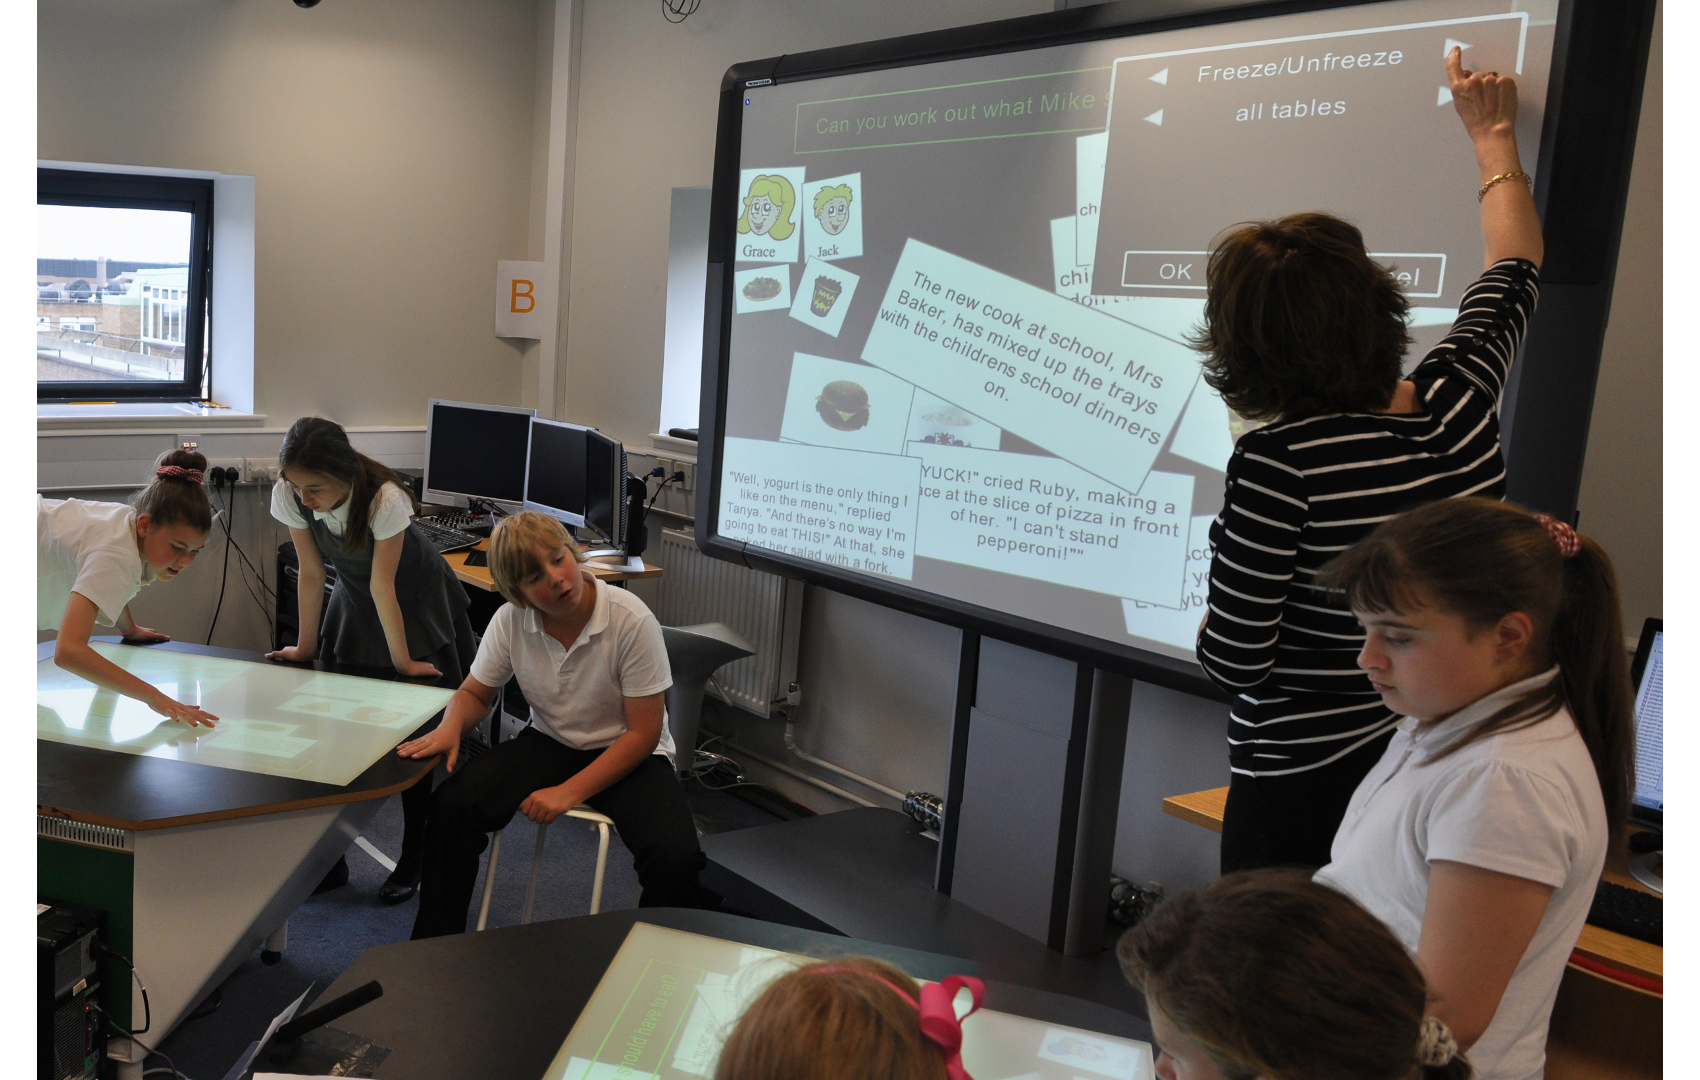
\includegraphics[width=\textwidth]{figures/study_board.png}
		\caption{The board interface.}
		\label{fig:studyBoard}
	\end{subfigure}
	\begin{subfigure}[t]{0.3\textwidth}
		\centering
		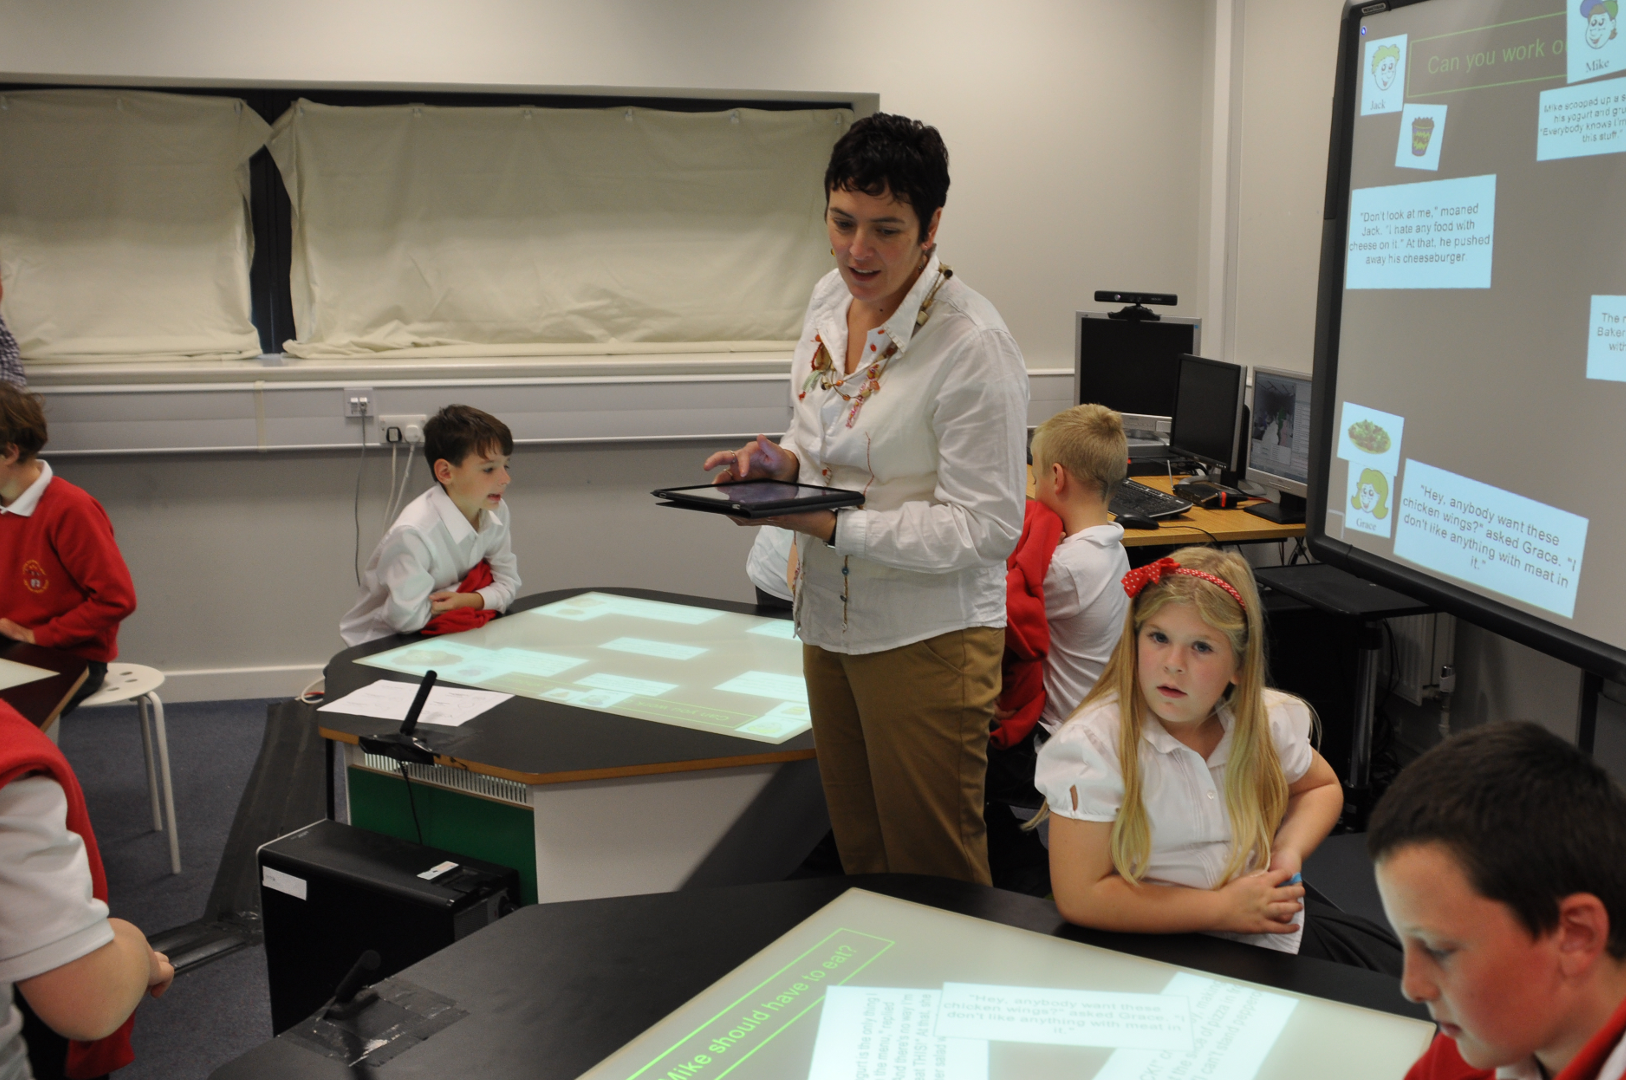
\includegraphics[width=\textwidth]{figures/study_tablet.png}
		\caption{The tablet interface.}
		\label{fig:studyTablet}
	\end{subfigure}
	\begin{subfigure}[t]{0.3\textwidth}
		\centering
		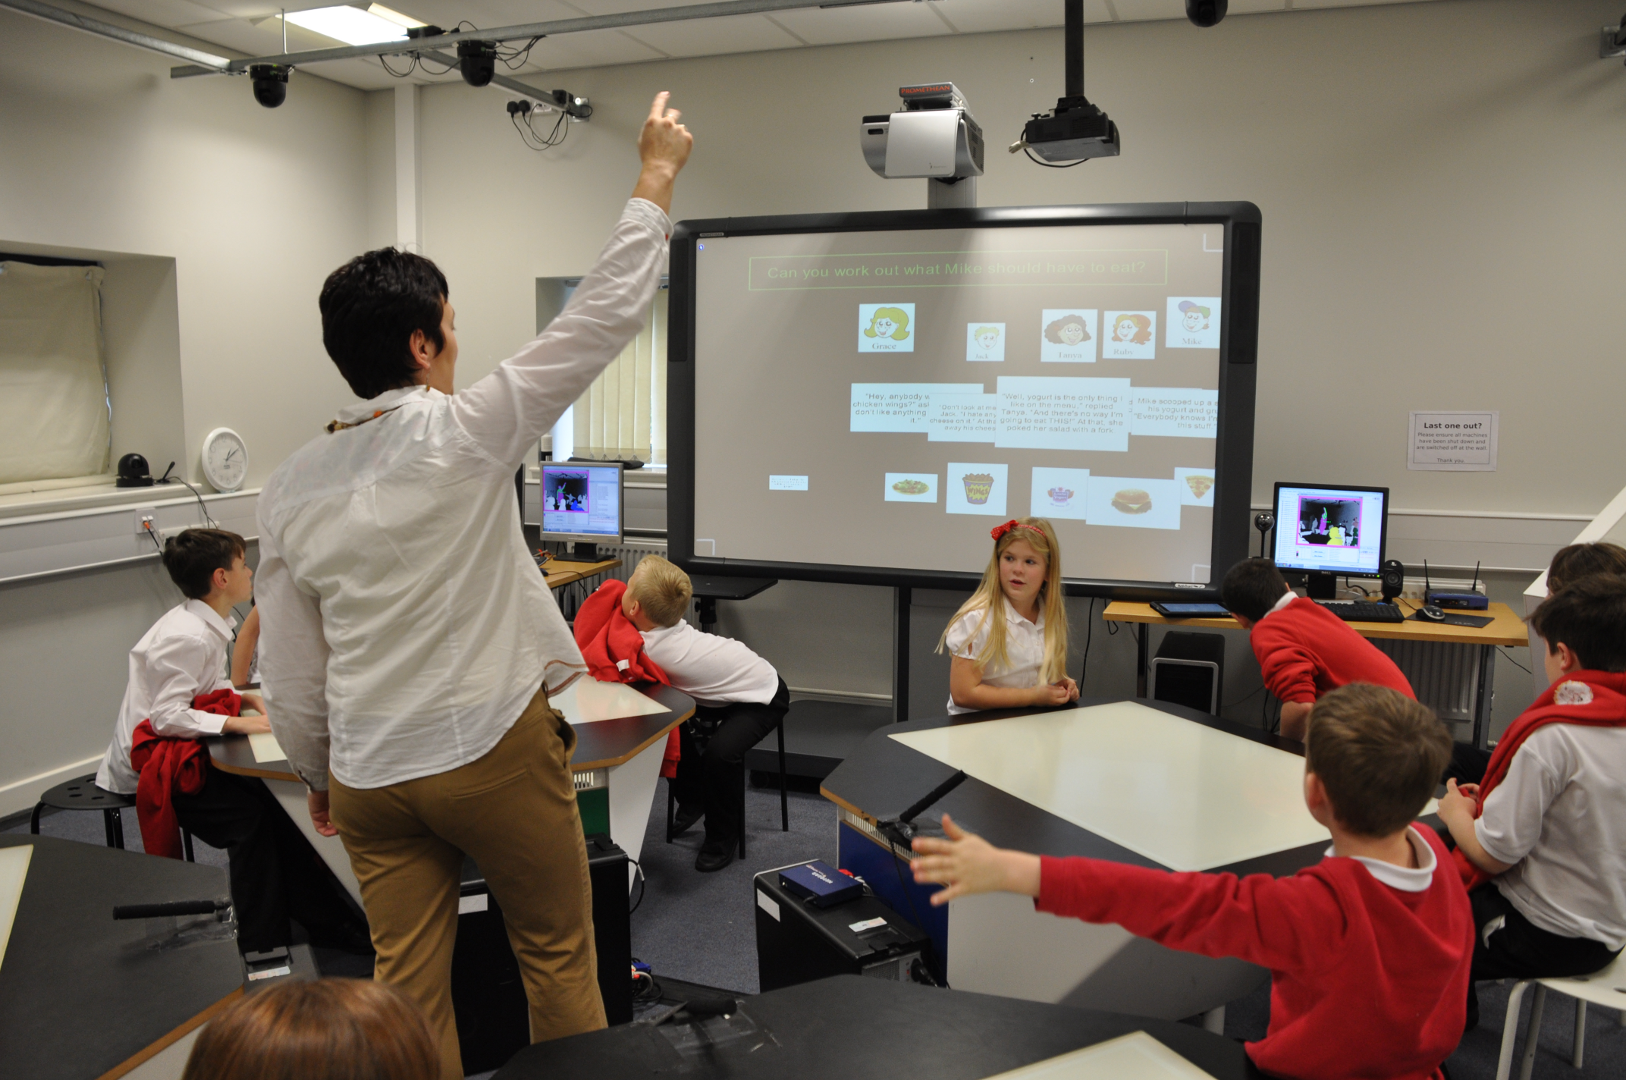
\includegraphics[width=\textwidth]{figures/study_kinect.png}
		\caption{The Kinect device.}
		\label{fig:studyKinect}
	\end{subfigure}
   	\caption{The use of interfaces and devices during the study to control instances of SynergyNet.}
   	\label{fig:studyDevices}
\end{figure*} 

\subsubsection{Task 1: Board Only}
\label{subsubsec:pilotStudyResultsTask1}

Ten commands were issued by the teacher during task 1's 25 minute and 46 second duration.
All these commands were issued through the interactive whiteboard as shown in Figure~\ref{fig:studyBoard}.
Out of these ten commands, one was issued incorrectly.
This was where the teacher intended to clear the board of content but instead cleared a student interface.
This false positive is likely due to the controls for orchestrating board content being positioned alongside the student-centric interface controls.
This led to the teacher confusing the two similarly worded command buttons.
The average time taken to issue a command with the board was 12.5 seconds with a standard deviation of 6.36 seconds.

\subsubsection{Task 2: Tablet Only}
\label{subsubsec:pilotStudyResultsTask2}

Nine commands were observed to be issued by the teacher in task 2's 18 minute duration.
All these commands were issued through the tablet interface as shown in Figure~\ref{fig:studyTablet}.
Of these nine commands, one was issued incorrectly.
This error was committed when the teacher intended to issue a command to a specific interface to show content on the board but instead showed content from all the student interfaces.
This false positive was likely due to the teacher leaving the \lq select all\rq\ option checked on the web-based controls from a previous command.

The average time taken to issue a command with the tablet was 13.6 seconds with a standard deviation of 11.7 seconds.
It was noted that the teacher would become preoccupied with the interface when issuing commands through the tablet and break interaction with the students to concentrate on using the device.

\subsubsection{Task 3: Kinect Only}
\label{subsubsec:pilotStudyResultsTask3}

Twenty one commands were observed to be issued by the teacher during task 3 in its 11 minute and 26 second duration.
All these commands were issued through the Kinect as shown in Figure~\ref{fig:studyKinect}.
The average time taken to issue a command with the Kinect was 6.6 seconds with a standard deviation of 5.59 seconds.
Of the twenty one commands issued during this task with the Kinect, eighteen were erroneous.

Six of these errors were caused by the teacher waving too many times.
This resulted in their third wave being interpreted as a command gesture.
The third wave was frequently interpreted as a pull gesture, which informs all the student-centric interfaces to show content on the board.
These false positives are technically the result of the teacher's failure to follow the command sequence but could be corrected by making the sequence more lenient for these types of mistakes.

Four of the errors were caused by the Kinect losing track of one of the teacher's hand.
Due to this, only one hand is identified as being above the teacher's head when in fact both are in the air.
This results in the gesture for the freeze command being interpreted as the gesture for sending content to the board.
These errors are the result of technical failures, caused by the limitations of the Kinect.

Two of the errors observed during task 3 were caused by the teacher trying to send contents to the tables when there was no content on the board to send.
These errors are the result of the teacher failing to follow instructions given during the training session and could have happened when using any of the control technologies.

Two of the errors were caused by the teacher performing a gesture before getting the Kinect's attention.
These false negatives were caused by the teacher not following the control sequence.

A teacher pausing for a relatively long time between getting the Kinect's attention and performing a gesture was the cause of one of the errors observed during this task.
The Kinect's attention is configured to expire if a teacher takes too long to perform a gesture.
As the teacher was made aware of the time-out mechanism beforehand, this false negative can be interpreted as an error caused by the teacher not following the control sequence.
The control sequence could be improved to accommodate for longer pauses by the teacher.

One of the erroneous commands was caused by the teacher intending to perform a freeze gesture.
The Kinect saw the movement of the hands moving from torso out from the wave gesture to get attention and interpreted it as the gesture for clearing the student interfaces.
This false positive results from a fault in the control sequence design.

Another observed error was caused by the teacher pausing in the middle of a gesture.
Without movement the Kinect saw the teacher performing a pose which issued a different command.
The cause of this false positive was the teacher failing to follow the control sequence since pausing during the gesture was equivalent to performing a different gesture in the view of the Kinect.

A single error was caused by the teacher performing the wrong gesture.
The teacher intended to freeze the tables but performed the pull content gesture instead. 
This error was caused by the teacher making a mistake.
This may indicate that the gestures are not intuitive and can lead to confusion.
The teacher had performed the pull gesture for retrieving the content from the board immediately before committing this error.
Repeating the first part of the control sequence; waving, may have led to them continuing with the same actions without realising the need to change the command gesture.

The Kinect was noted to have experienced several issues which may account for the observed errors in the command sequence.
The Kinect lost track of the teacher's calibration three times.
In addition to this, the teacher presence was lost entirely by the Kinect three times.
It was also noted that the Kinect could not allow the teacher to calibrate when they were stood in specific places despite being within the range of its view.
This was potentially due to the Kinect's view of the teacher being partially obscured by students moving about the tabletop interfaces.

The teacher spent the majority of the task trying to unfreeze the tables.
The repeated errors prolonged this process which would usually require a single command.
Due to the high number of errors caused by the Kinect, students became frustrated.
There appeared to be two causes of the majority of the errors:

\begin{itemize}
\item The teacher was waving too much when obtaining the Kinect's attention.
\item The Kinect repeatedly lost track of the teacher and their limbs. 
\end{itemize}

The high frequency of commands compared to the previous tasks was partially due to attempts to correct errors.
The teacher had to repeat gestures which failed or issue additional commands to amend undesirable consequences from the erroneous gestures.

Three of the errors noted during this task could be categorised as false negatives whereas eight of the errors were false positives.

\subsubsection{Task 4: All Devices}
\label{subsubsec:pilotStudyResultsTask4}

For task 4, where the teacher had the option of using any of the three control devices, five commands were observed to be issued by the teacher in its 11 minute and 38 second duration.
Three of these commands were issued through the board control and two through the Kinect.
The tablet was used for issuing no commands, despite being available to the teacher.
Out of these five commands, two were issued incorrectly.
These two erroneous commands were both issued using the Kinect.
The first of these erroneous commands was caused by the Kinect confusing gestures.
After waving the teacher moved their hands together intending to perform the gesture for the screenshot command.
However, the Kinect saw the hands moving from the wave gesture used to get attention towards the torso and interpreted it as the gesture for pulling content from the board.
This is a problem in the control sequence.
The Kinect sees the movement of the teacher's hands between waving and the command gestures.
The Kinect node then interprets this movement as a different command gesture.
The second erroneous command was caused by the teacher waving too many times to retrieve the Kinect's attention.
The teacher's third wave is interpreted as a command gesture rather than ignored after the Kinect focuses on the teacher.
Both of these errors can be categorised as false positives.

During this task the average time taken to issue a command with the board was 12.1 seconds with a standard deviation of 4.05 seconds.
The average time taken to issue a command with the Kinect was 6.5 seconds with a standard deviation of 1.38 seconds.

\subsection{Observations}
\label{subsec:pilotdiscussion}

% // TODO Note how the Kinect's poor range and tracking of movement were hugely problematic and needed to be corrected for any further phases.


% From Discussion 1 ===========================================================================

% // TODO Trim down.

\begin{table}[h]
\begin{tabular}{!{\vrule width 1.5pt}c|c|c|c!{\vrule width 1.5pt}}
\noalign{\hrule height 1.5pt}
\multicolumn{1}{!{\vrule width 1.5pt}c!{\vrule width 1.5pt}}{\textbf{}}	
&\textbf{Number} &\multicolumn{1}{!{\vrule width 1.5pt}c!{\vrule width 1.5pt}}{\textbf{Number}}	 &\textbf{Average Time}\\
\multicolumn{1}{!{\vrule width 1.5pt}c!{\vrule width 1.5pt}}{\textbf{}}	
&\textbf{of} &\multicolumn{1}{!{\vrule width 1.5pt}c!{\vrule width 1.5pt}}{\textbf{of}}	 &\textbf{to Issue}\\
\multicolumn{1}{!{\vrule width 1.5pt}c!{\vrule width 1.5pt}}{\textbf{Device}}	
&\textbf{Commands} &\multicolumn{1}{!{\vrule width 1.5pt}c!{\vrule width 1.5pt}}{\textbf{Errors}}	&\textbf{Commands}\\
\noalign{\hrule height 1.5pt}
Board 					&13 					&1				&12.4 seconds				\\
\cline{1-4}
Tablet 					&9						&1				&13.6 seconds				\\
\cline{1-4}
Kinect 					&23 					&20			&6.59 seconds				\\
\noalign{\hrule height 1.5pt}
\end{tabular}
\caption{The usage of the control devices in the study.}
\label{table:results1}
\end{table}

Table~\ref{table:results1} summarises the usage of the three control technologies used in the study.
The results showcase the strengths of each of the technologies in places.
The board device was shown to produce the least errors over use whereas the tablet and Kinect devices were shown to provide shorter interaction times.
The device which was quickest for issuing commands was the Kinect as shown in Figure~\ref{fig:averageTime}.
However, the increasing interaction times as the study progressed could be in part attributed to the teacher gaining experience with the system over the tasks.

\begin{figure*}[t]
	\centering
	\begin{subfigure}[t]{0.45\textwidth}
		\centering
		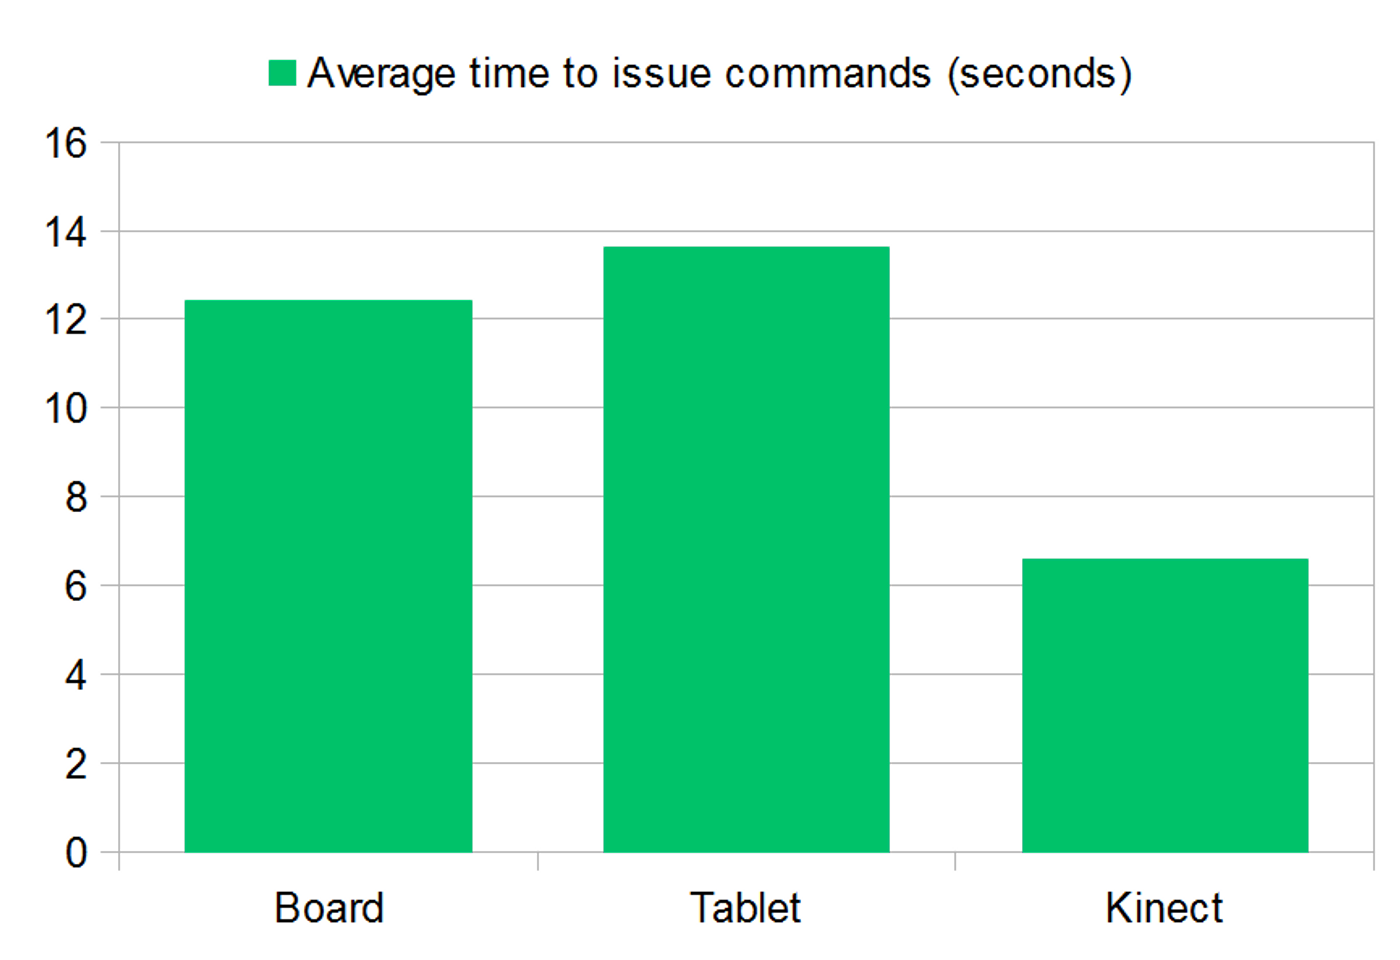
\includegraphics[width=\textwidth]{figures/bar_chart_average_time.png}
		\caption{Average time taken to issue commands.}
		\label{fig:averageTime}
	\end{subfigure}
	\begin{subfigure}[t]{0.45\textwidth}
		\centering
		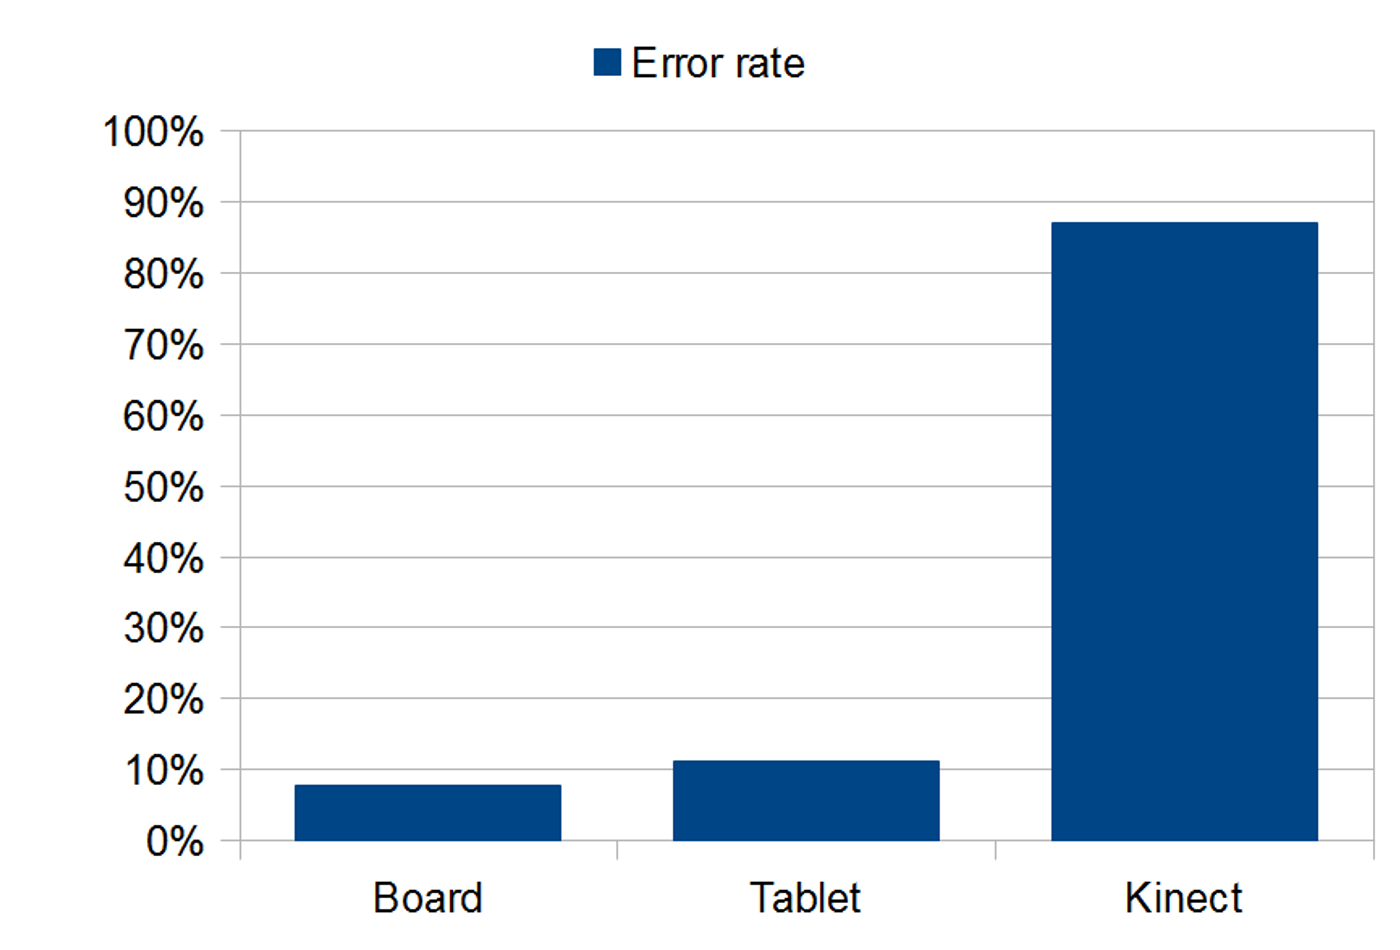
\includegraphics[width=\textwidth]{figures/bar_chart_error_rate.png}
		\caption{Percentage of erroneous commands.}
		\label{fig:errorRates}
	\end{subfigure}
   	\caption{Comparison between each control technology.}
   	\label{fig:graphs}
\end{figure*} 

Several shortcomings of the devices became evident throughout the study.
Both the board and the tablet were noted to take the teacher's focus away from the students.
The distraction of these devices was exacerbated by the fact that both required relatively longer interaction times the Kinect.

The most problematic device was the Kinect as shown in Figure~\ref{fig:errorRates}.
The majority of actions performed using the upper-body gestures through the device resulted in erroneous consequences such as the wrong command being issued.
There are several potential causes of these errors.
The first stems from the training of the teacher participating in the study.
The one hour training may not have been enough time to allow the teacher to gain familiarity with the control devices.
This may have contributed a number of failures to follow the command sequences, especially with the Kinect.
In addition to this, the Kinect encountered several technical issues which prevented it from accurately tracking the teacher, their limbs and their joints.
This inability to track could have been caused by the teacher leaving the Kinect's field of view.
The classroom environment set up in the lab in which the study took place was larger than the Kinect's range.
Due to this, the teacher often wandered beyond the Kinect's range to monitor and talk to students positioned around the distant tabletop interfaces.
Whenever the teacher travelled outside the Kinect's field of view for more than several seconds the Kinect would lose track of their calibration and identity.
This meant that the teacher would need to establish their teacher status on re-emerging into the Kinect's view and would need to perform the calibration pose again.

The Kinect is capable of regaining their identification of a person if they appear in the same area in a similar pose within three seconds of their disappearance.
These momentary loses were noted to occur several times in the study and were noted to be the potential cause of the device incorrectly identifying gestures.
However, for the majority of occasions where the Kinect stopped tracking the teacher, the loss was permanent and required the teacher to recalibrate.

Even when the teacher stayed within the Kinect's field of view, technical issues relating to the device's range caused errors.
If the teacher was positioned close to the limits of the Kinect's range performing gestures, the device's limb and joint tracking became inaccurate.
The device would often lose track of the teacher's limbs and joints, seeing them either move erratically or appear at rest when in fact the teacher was moving them to perform a gesture.
When a limb was obscured the Kinect would attempt to position it, often resulting in an inaccurate placement.
This also led to the limb positions moving erratically which caused several of the errors in the gesture recognition system.

A number of the errors that occurred when the Kinect was used were established to be caused by the design and implementation of the control sequence.
The majority of these relate to the movement of hands immediately after obtaining the Kinect's attention.
The movement of the teacher's hands when finishing the attention-grabbing wave gesture were on occasion interpreted as a separate command gesture.
In addition to this, the Kinect often interpreted the movement of hands to positions needed to perform a command gesture as the command gesture itself.
These errors could be corrected with the implementation of a pause in the control sequence after the Kinect's attention is gained.
The pause would allow the Kinect to ignore any unintentional gestures performed in the transition between the completion of the wave gesture and the command gesture.

The number of false positives which occurred during the use of the system outweighed that of false negatives.
In total, ten errors committed while issuing commands with the Kinect could be categorised as false positives throughout the study.
Though the attention-toggling approach used in the command sequence was intended to reduce false positives there are still scenarios in which they can occur.
Movement between gestures and the teacher pausing while the Kinect's attention was active was the cause of these false positives.
The suggested improvements to the control sequence of adding pauses may reduce the number of these false positives.

In relation to false positives, relatively few false negatives were observed during the study.
All three instances of errors which could be categorised as false negatives occurred as a consequence of the teacher failing to follow the control sequence.
Improvements to the training a teacher receives prior to using the system could reduce the occurrences of these errors in the future.

Efforts were made to ensure the software interfaces for the three control technologies used were similar.
The controls for the board and tablet used the same set of control components but different layouts.
Though the technical capabilities of these two interfaces were the same, the differences in their appearances could have been a confounding factor.
In addition to this, both the interfaces differ from control sequence used for the gesture controls.
The use of a new set of controls with the same appearance on both the tablet and board interfaces which resemble the control sequence may improve cohesion between the technologies.

After the study, the participating teacher was asked to discuss their preferences regarding the devices used.
The teacher stated that they favoured the use of the Kinect.
This was because it was quick and didn't require them to hunt through the interface to find the relevant controls.
However, they were disappointed in the number of errors it produced.
The teacher stated that the tablet device was the least preferred device due to the complexity of the web interface.
This is the reason why the teacher did not use it during task 4.
Despite the board being the most used device with the least amount of errors throughout the study, the teacher had no preference for or against its use.
The teacher stated that during task 4 the board was used as a fall-back when issuing commands through the Kinect continued to produce errors.

The high error-rate observed in the study indicates the need for improvements.
The study was originally intended to involve more than a single teacher and class but once the error-rate became apparent it was decided that studies should be postponed until improvements were implemented.
The improvements proved to be significant enough to warrant being discussed separately in future work alongside the studies using them.
% From Discussion 1 ===========================================================================


% From Conclusion 1 ===========================================================================

% // TODO Trim down.

% // TODO Remove paper summaries.

% // TODO Remove discussions of what to do next.

The primary objective of the study was to find how the use of upper-body gestures compares to alternative classroom control technologies.
The Kinect was shown to be the quickest despite the errors encountered.
The board appeared to be the most intuitive due to its relatively low count of errors.
However, the teacher did express a preference for the Kinect device stating that they found it easier to keep track of the students when using it.
In addition to this, the speed of issuing commands through the Kinect could be used to argue that it may have been more intuitive than the other devices.
However, the frequent errors relating to the teacher not following the Kinect's command sequence imply that its use is not intuitive enough to be used with confidence in the classroom.

The study hypothesis state that the gesture controls would allow commands to be issued quicker and with fewer errors due to their intuitiveness.
However, the high error rate and interruptions to the class caused by the teacher needing to repeat the commands proved this to be incorrect.
For the successfully issued commands from the gesture controls, observations on interaction between the teacher and their students conformed to the hypothesis that the Kinect would be the least intrusive.
The teacher would often focus entirely on the board or tablet during their use but could continue conversations with the students when attempting to issue commands through the Kinect.
However, the error-rate is too high to allow for conclusions to be drawn from these observations.

Despite the teacher's preference for the Kinect device, its use has been shown to be problematic.
Through using the improvement of a pause during the control sequence, as suggested in Section~\ref{subsec:pilotdiscussion}, a number of these errors could be countered.
However, the errors resulting from the limitations of the Kinect, such as those caused by the Kinect tracking the user's limbs and joints inaccurately at locations in close proximity to the extremes of the device's range, would still be present in the future use of the system.
There are several possibilities which could be considered for overcoming these limitations.
The most obvious of these is to use an alternative sensing technology capable of tracking a user's upper-body.
The set of gestures used in the current system could be reused with a different depth sensing device~\cite{Kean2011}.

When considering alternative technologies for use in detecting upper-body gestures, the reasons for the Kinect's original adoption should be kept in mind; cost, adaptability, accuracy, un-encumbering nature and responsiveness.
Any alternative device providing gesture recognition for teachers should conform to these criteria.
Despite one of the benefits of the Kinect being its un-encumbering nature, an alternative technology which requires a wearable device could be feasible~\cite{Rekimotoa,Zhu2011}.
If the device is un-intrusive enough to allow the teacher to freely move about the classroom and interact with students while issuing commands it could be used with SynergyNet and the criterion relating to un-encumbering nature could be disregarded. 

Future work could include augmentations to the SynergyNet framework to overcome the limitations of the Kinect.
One such augmentation could be the use of multiple Kinects to accurately monitor a larger area.
If the area accurately monitored by the Kinect is expanded to cover the entirety of a classroom, the teacher would then be capable of issuing commands through upper-body gestures anywhere in the environment.
Though there are many issues with the use of multiple Kinects~\cite{Maimone2012,Schroder2011} there are several potential methods which allow them to work together~\cite{Wang2012}.
If SynergyNet is made capable of combining user data from multiple Kinect devices it should be possible to track teachers moving across the device's monitored areas.

As discussed in Section~\ref{subsec:pilotStudyImplementation}, the decision was made not to implement a method of interface selection.
This was due to the fact that the most popular method of interface selection in the focus group would be problematic when implemented into a system with only a single light-coding device.
With the use of multiple Kinects this issue may be overcome. 
The implementation of support for multiple Kinects in future systems would allow the teacher to select tables without the need to move to them through the use of the pointing gesture without obstruction.
This would allow teachers to perform the entire command sequence without moving from their current location.

To limit the errors cause by the Kinect losing track of the teacher's limbs and joints, automatic calibration could be implemented~\cite{Bellmore2011}.
This would allow the teacher to issue commands through the upper-body gesture control sequence without performing the calibration pose beforehand.
The Kinect could also be augmented to perform user recognition~\cite{Leyvand2011}.
This would allow the Kinect node to automatically identify which persons in the classroom are teachers.

Despite the majority of errors relating to the gesture set originating from issues with the technology, a number of the errors were observed to originate from the design of the gesture set and its control sequence.
These errors indicate that some of the gestures are not intuitive despite their user-generated nature.
Therefore, to reduce the number of errors, improvements to the gesture set could be made.
As identified in Section~\ref{subsec:userGeneratedGestures}, there is a trend for most of the gestures to conform to a metaphor.
However, a number of gestures do not conform to this trend.
The intuitiveness of the gesture set as a whole may be impeded by this sub-set of non-metaphor based gestures.
One such non-metaphoric gesture is the raised single hand pose used to send content on student-centric interfaces to a board.
Changes to make the gesture set more cohesive could improve the gestures' intuitiveness and reduce the error rate of their use.

The lack of cohesion in the gesture set may have derived from decisions made in the design of the focus group study.
Applying constraints on the gestures to be performed and allocating gestures based on command priority rather than their popularity may have contributed to the lack of cohesion.
The results of the study could be reconsidered in future studies using a different analysis approach which ignores the command priority.
The focus group study could also be repeated without the constraints placed on the gestures the participants perform.

In addition to repeating the focus group study, the study utilising the various control technologies could also be repeated.
With the implementation of several of the suggested improvements, such as the use of multiple Kinects, automatic calibration and changes to the gesture control sequence, many of the errors relating to the use of the Kinect could be resolved.
This would make the results of future studies much more indicative of whether the use of upper-body gestures is suitable for controlling classroom technologies with.
These future studies could benefit from the use of more than one teacher to allow for the results to be more indicative.
The use of multiple teachers will also allow for changes in the task ordering to remove experience with the system as a confounding factor.

\begin{table}[h]
\begin{tabular}{!{\vrule width 1.5pt}c|c!{\vrule width 1.5pt}}
\noalign{\hrule height 1.5pt}
\multicolumn{1}{!{\vrule width 1.5pt}c!{\vrule width 1.5pt}}{\textbf{Criterion}}	
&\textbf{Determined by} 	\\
\noalign{\hrule height 1.5pt}
Cost 					& 					\\
\cline{1-1}
Adaptability 				&Sensing 			\\
\cline{1-1}
Accuracy 				&Device 				\\
\cline{1-1}
Un-encumbering Nature	&(Kinect) 			\\
\cline{1-1}
Responsiveness 			& 					\\
\cline{1-2}
Lexicon Size 				&Control Sequence 	\\
\cline{1-2}
Intuitiveness 			& 					\\
\cline{1-1}
Comfort 					& 					\\
\cline{1-1}
Low Mental Load 			&Gesture Set 		\\
\cline{1-1}
Interaction Space 		& 					\\
\cline{1-1}
Ubiquity 				& 					\\
\noalign{\hrule height 1.5pt}
\end{tabular}
\caption{The adhesion of the gesture set's implementation to the upper-body gesture criteria.}
\label{table:criteria}
\end{table}

Table~\ref{table:criteria} summarises criteria outlined for evaluating an upper-body gesture system outlined in Section~\ref{subsec:gatheringGestures} which was derived from the requirements defined by Waches et al.~\citeyearpar{Wachs2011}.
The table shows which elements of upper-body gesture system the criteria apply to.

As discussed in Section~\ref{subsec:gatheringGestures}, the criteria relating to the capabilities of a sensing technology for upper-body gestures are; cost, responsiveness, adaptability, accuracy and un-encumbering nature.
The implemented system used in the study's adherence to these criteria was determined by the technical specifications of the Kinect device.
Though low-cost, responsive, adaptable and un-encumbering, concerns about the device's accuracy during the user study were raised.
A better trade-off between accuracy and the other device-determined criteria may be found through an alternative.
The suggested improvements of using a different light-coding device or multiple Kinects could aid the system in meeting the criterion of acceptable accuracy.

The criterion relating to the lexicon size can be said to be met by the gesture-set produced in this paper.
This is because the gesture set is the same size as the minimum typical short-term memory limit as discussed in Section~\ref{subsec:gatheringGestures}.

The user-study provides evidence that the implemented gesture set, despite conforming to some of the effective gestures criteria, needs improving:

\begin{itemize}
\item \textit{{Intuitiveness:}}  The teacher was able to remember and naturally perform the majority of gestures in the correct sequence for issuing their desired commands.
However, the teacher did occasionally fail to follow the gesture sequence.
This could be improved through more intensive training before use or creation of a more cohesive gesture set.
\item \textit{{Comfort:}}  No issues concerning discomfort caused through the performance of upper-body gestures were identified during the study.
It is possible that prolonged use of the device could cause fatigue.
This should be investigated in future studies.
\item \textit{{Low mental load:}}  The teacher was often able to quickly execute the issuing of commands through upper-body gestures.
However, the teacher on several occasions paused during the control sequence, causing some of the issues discussed in Section~\ref{subsec:pilotStudyResults}.
In the post-study interview the teacher explained the pauses were caused by their concentration on remembering which gesture should be performed next.
This indicates that improvements could be made to the gesture set and the control sequence to reduce mental load.
\item \textit{{Interaction Space:}} The failure of the Kinect to recognise many of the gestures performed occurred due to the device losing track of joints which left its accurately monitored area.
This implies that the gestures and classroom environment require more interaction space than the device is capable of.
The use of a different light-coding device or multiple Kinects could increase the device's range to accommodate for the system's required interaction space.
\item \textit{{Ubiquity:}} In the post-study interview the teacher discussed how all the gestures used were similar enough to typical classroom actions performed by teachers that they did not feel out of place.\\ 
\end{itemize}

The use of only one teacher in the study limits the scope of this work's findings.
The initial results show promise but were impeded by issues relating to the accuracy of the Kinect.
To overcome the limitations of the evaluation of the implemented control system, future work will entail repeating the study with a greater number of teachers and improvements to the sensing technology.

Both the gesture set presented in this work and its implementation, despite requiring improvements, have shown enough potential to warrant further work.
The gestures and control sequence presented could be used to control various classroom technologies through the use of a light-coding device.
The ability for teachers to quickly issue commands without breaking discussion with their students made feasible by a light-coding device, as observed with the implemented system's use in the study, is desirable for technology-rich classroom environments.
The implementation of the suggested improvements to resolve the observed errors could make upper-body gestures an effective method of managing classroom technology.
% From Conclusion 1 ===========================================================================


% From Background 2 ===========================================================================

% // TODO Trim down - can remove most of this section as its just summarising the first half of the paper.

\subsubsection{Issues with Initial Upper-body Gesture Controls}
\label{subsubsec:pilotdiscussionIssues}

Previous studies involving the use of SynergyNet's upper-body gesture controls revealed several shortcomings.
To assess the existing implementation a set of criteria for upper-body gestures was derived from the requirements for hand gestures outlined by Wachs et al.~\cite{Wachs2011}.
These criteria assessed the system's cost, adaptability, accuracy, un-encumbering nature, responsiveness, lexicon size, intuitiveness, comfort, mental load, interaction space requirement and ubiquity.

The previous study has revealed four criteria in which SynergyNet's upper-body gesture controls needs improvement; 
\textit{accuracy}, \textit{interaction space}, \textit{intuitiveness} and \textit{mental load}.
Using observations from the previous study it is possible to identify several issues which resulted in the system being incapable of meeting these three criteria.

\begin{itemize}

\item \textbf{Issue 1: Losing Track of Users, Limbs and Joints}\\
For SynergyNet, issues relating to accuracy and interaction space originated from the Kinect device.
The device was noted to lose track of users which had the result of any persons carrying teacher status to lose their ability to issue commands.
This would require the teacher to repeat designating their teacher status and performing the calibration pose.
This was problematic due to its time consuming nature and was noted to occur when a teacher left the Kinect's field of vision.
The Kinect's range is limited to three and a half metres~\cite{Maimone2011} and a sixty degree viewing angle~\cite{Stone2011}.
This is too small to monitor an entire typical classroom environment.
In addition to this the Kinect often lost track of teacher's limbs and joints.
It was noted this occurred towards the limits of the Kinect's field of view.
This was because the Kinect's accuracy decreases in proximity to the limits of its view~\cite{Mehrotra2011}.
Gestures would either be interpreted incorrectly as other gestures or were totally ignored by the system due to this lack of accuracy.

\item \textbf{Issue 2: Gesture Confusion}\\
SynergyNet's failure to meet the criterion for intuitiveness in the previous study was, in part, caused by repeated errors committed by the teacher performing the wrong gestures when intending to instigate specific commands.
The teacher stated that they would often forget which gestures related to which command.
This indicated that the gestures were not intuitive enough.
In addition to this the teacher's confusion of gestures also attributed to the system's failure to meet the criterion for mental load.
The teacher stated in an interview after the previous study that they forgot the gestures needed for specific commands on a number of occasions.

\item \textbf{Issue 3: Stringent Control Sequence Requirements}\\
The numerous steps in the control sequence that the teacher is required to repeat on various occasions, such as calibration and establishing their identity, is a contributing factor to the system's failure to meet the criterion for mental load.
SynergyNet's failure to meet the criterion for a low mental load was identified during previous use of the system where teachers would often pause during the command sequence.
The control sequence required teachers to execute the command sequence without any pauses.
This resulted in a number of errors where the Kinect's attention would time-out or the system would interpret the pose the teacher paused in as a command gesture.
The teacher stated that they paused because they were concentrating on recalling the appropriate gesture for the command they intended to execute.
This indicates that the mental load required by the current system implementation is too large.
In addition to this the unexpected results of the system wrongfully interpreting gestures due to teacher's failing to meet the control sequence's stringent requirements are detrimental to its intuitiveness.

\item \textbf{Issue 4: Reduced Functionality}\\
There may be circumstances where the teacher wishes their action to affect only a specific subset of the student's interfaces.
The results of the guessability study performed to generate the initial upper-body gesture set and control sequence to be used by SynergyNet indicated a pattern in participant's preferences towards selection.
It was noted that participants would prefer to point at specific interfaces if wishing a command to only affect them.
A pointing gesture was proposed but not implemented due to the issue of a teacher's body potentially obscuring the interfaces being pointed when a single Kinect is used.
Without an interface selection method, the Kinect controls offer less functionality than the alternative static and mobile interfaces.
Because any command issued with the Kinect must influence all interfaces, teachers must put additional thought into its use.
The lack of cohesion between the Kinect controls and alternatives may exacerbate the identified problems concerning intuitiveness and mental load.

\end{itemize}
% From Background 2 ===========================================================================

\section{Study}
\label{sec:study}

% // TODO Small intro to study (referring back to similar structure of the pilot)

\subsection{Resolving Issues}
\label{subsec:studyResolvingIssues}

% // TODO Trim down and make suitable.

The issues outlined in Section~\ref{subsubsec:pilotdiscussionIssues} were noted in the previous phase of the study to make the use of the system counter-productive.
The benefits afforded by the system of non-intrusive and quick command execution were made irrelevant due to the high number of errors caused by the identified issues.
Resolving these issues could allow the system to function as intended and would allow the potential benefits of the upper-body gesture controls to be evaluated and employed.

\subsubsection{Resolving Issue 1: Improving the System's Tracking}
\label{subsubsec:studyResolvingIssues1}

To improve the accuracy and interaction space of the sensing technology used with the system, multiple Kinects could be employed.
With more Kinect devices in the environment, more of the classroom would be monitored.
A larger monitored area reduces the chance of the teacher losing their calibrated status by wandering out of the Kinects' view.
This saves time by reducing how often the teacher needs to repeat the calibration process.

Dubois et al.~\cite{Dubois2011} track the movement of mobile objects through an apartment using two Kinects.
Using knowledge of the Kinects' positions relative to each other, their visual and depth information can be stitched together.
Any processing applied to the information provided by the Kinect to track the movement of mobile objects can then be applied to the combined output.
Stitching the information requires a large amount of processing power.
However, once done it allows for the later process-intensive functions used to identify and track mobile objects to be applied just once, rather than having separate process-pipelines for each Kinect.

Luber et al.~\cite{Luber2011} utilise multiple Kinects in their work to track persons across large environments.
Through a form of user recognition the system presented is able to track a person as they cross from one Kinect's field of view to another.
The system tracks the movement of persons across their viewed areas.
On the Kinect identifying a person the system determines their unique visual and geometric features.
Whenever a new person is identified on a Kinect the system checks to see if they have been seen before on another Kinect by comparing their features.
If so the system can then establish the movement of persons across multiple fields of view.
This allows for a person's movement to be tracked across a larger area.

Overlapping the views of the Kinects would eliminate the need for teacher's to perform gestures towards the limits of a single Kinect's view.
This ensures that teachers stay within the areas of the Kinects' view which are more accurate.
However, when the views of two or more Kinects overlap there is the potential issue of interference~\cite{Satyavolu2012}.
The two multiple Kinect systems discussed so far~\cite{Dubois2011,Luber2011} avoid this issue by ensuring that the overlapping area of Kinect views is minimised.
The Kinect functions by projecting a pattern of infra-red light.
Because all Kinect devices produce, and look for, this light pattern at the same frequency it is possible for one Kinect device to see the pattern produced by another.
The Kinects cannot distinguish the infra-red light patterns and will interpret the pattern from another Kinect as its own.
The Kinect uses deformations in their projected pattern to detect the placement of objects.
If two patterns overlap the Kinect will not be capable of accurately identifying these deformations and their implications.
This interference can significantly reduce the accuracy of Kinect devices~\cite{Satyavolu2012}.

To avoid multiple Kinects viewing each other's patterns, the sensing devices can be positioned in perpendicular planes~\cite{Caon2011,Kramer2012}.
Positioned ninety degrees from another Kinect ensures that it will not view any of the infra-red light projected direct from the other device.
This positioning will also minimise the amount of infra-red light the Kinect sees from the surfaces the other device's pattern is projected onto.
This reduces interference to a level where the Kinect is capable of accurately tracking persons' limbs and joints~\cite{Caon2011}.
The setup used by Dubois et al.~\cite{Dubois2011} also entails positioning the two Kinects used perpendicular to each other so that either Kinect cannot see the other's projected pattern.
This approach does increase the accurately monitored area of a system of Kinect devices but does have a restriction; only two Kinects can have overlapping views.
If more than two Kinects are positioned perpendicular to its neighbours then at least two of the devices will be in parallel.
This means that the two parallel devices' will interfere with each other, reducing their accuracy.

A potential technique of using multiple Kinects together without their projected patterns interfering with each other is time division~\cite{Schroder2011}.
This is where the Kinects in a system will take it in turns to project and view their patterns.
Any pairing of Kinects which cause interference can be set up so that they never project at the same time.
However, a Kinect will not be collecting any usable depth information while another Kinect which could interfere with it is projecting.
Due to this,  the technique causes a reduction in the frame-rate of the depth image collected from the devices.
The accuracy of the devices afforded by removing interference is traded-off for a reduction in responsiveness.
Therefore, the adoption of this technique, while resolving the issue of accuracy may result in the system being unable to meet the criteria for responsiveness.

Another potential technique of reducing the interference caused by overlapping light patterns is the movement of the sensing devices~\cite{Maimone2012}.
By moving a Kinect, the device's projected pattern is moved along with its camera.
If no other device is currently performing the same motion the system should be capable of identifying the reflected light from a unique Kinect.
This has been shown to reduce interference when multiple Kinects are used together~\cite{Maimone2012} but does have the requisite that the devices are constantly in motion.
Large movements which change the Kinects' locations may complicate any calculations which utilise the positional information provided by the devices.
Positional information derived by the Kinect is relative to its cameras.
Therefore, when information between multiple Kinects must be used together, knowledge of the Kinect's positions relative to each other must be known.
This allows the positional information to be made relative to the physical environment the Kinects occupy.
Constant movement of the devices would require additional calculations to transform the relative positional information output from a Kinect to their real-world locations.
This additional calculation could reduce the system's responsiveness.
Vibration of the Kinect could be used to minimise the movement required to differentiate the devices' projected patterns~\cite{Kainz2012}.
However, to add any motion to the Kinect devices, extra cost must be spent to implement the motors needed to automate this movement.
The adoption of this technique, while resolving the issues relating to accuracy and interaction space, may result in the system being unable to meet the criteria for cost.

To differentiate the infra-red light produced and received by the Kinect devices, filters could be employed.
Multiple depth-cameras using the same structured light setup as the Kinect have been made capable of working together through filtering the infra-red used~\cite{Kim2008}.
However, the Kinect is not capable of this~\cite{Kainz2012}.
The Kinect produces and views a very small range of infra-red frequencies.
Filtering this would reduce the range of frequencies visible to each Kinect further and would likely result in the depth image becoming more inaccurate.
This is due to further loss of reflected light through its frequency shifting beyond the device's range.

The techniques discussed so far for allowing multiple Kinect devices to work together involve providing methods of differentiating the devices' projected light patterns.
Wang et al.~\cite{Wang2012} present a potential technique which reduces the influence of interference caused by multiple Kinects not through prevention but correction.
The technique uses the depth information collected from the devices to reconstruct the scene viewed.
In areas where the depth information is missing due to interference, a plane-sweeping based algorithm is used to regenerate the lost information.
The algorithm uses the existing depth data from all the Kinect devices to calculate the missing information.
The initial results shown from Wang et al.'s~\cite{Wang2012} simulations are promising but there may be issues with using this technique in a real-world scenario.
The time and processing power required by the algorithm could reduce the system's responsiveness.

Alternative depth sensing technologies could be used to track the movements of the teacher in a classroom.
These alternatives may resolve the issues relating to accuracy and interaction space but could incur other issues.
The Primesense~\cite{Wilson2010} depth camera performs the same function as the Kinect and could be used with SynergyNet.
However, the device has a similar range to the Kinect and would therefore require several to be used together to increase their observed area.
Because the devices use the same structured light technique as the Kinect the same issue of interference would still be present.
Oblong's Mezzanine~\cite{kramer2011} uses custom built depth cameras to observe user's movement in a meeting room environment.
The system's range is greater than that of a single Kinect but its cost far exceeds that of several of Microsoft's devices.

\subsubsection{Resolving Issue 2: Improving Gestures}
\label{subsubsec:studyResolvingIssues2}

To improve the intuitiveness of the SynergyNet upper-body gesture system it is possible that a number of the gestures may need to be changed.
The previous study indicated that there was a subset of gestures which caused more problems than the rest.
Waving to get the Kinect's attention and holding one hand up to send content to the board were both noted to be problematic.
As noted in the previous study, both these gestures do not conform to a pattern common to the others where the gestures relate to related real-world actions.
For example, the gesture of pulling to retrieve content from a display to the classroom tabletops relates to the real-world of pulling items towards a location.
Where a gesture acts as a metaphor for a real-world action its intuitiveness is enhanced~\cite{Wang2008}.
Because the real-world action and the context of its use are already known to users, a similar gesture requires minimal additional training.
Both waving and holding one hand up are the only gestures in the set which bear no relation to related real-world actions.
Changing these gestures to ones resembling related real-world actions may improve their intuitiveness.

It is possible that many of the errors committed in the previous study may have been avoided if the teacher participating had better training with the system.
In the previous study the teacher had a single hour to learn how to use SynergyNet, including the static, mobile and Kinect controls.
It is possible that this may not have been enough time for the teacher to gain sufficient confidence with using the system.
The training session took place immediately before the previous study.
The teacher may not have had enough time to memorise how to orchestrate using the three control technologies, specifically the Kinect.
Giving the teacher time after the training session to reflect on and memorise what they've learnt may allow their use of the system in the future to be less error-prone.

\subsubsection{Resolving Issue 3: Improving the Control Sequence}
\label{subsubsec:studyResolvingIssues3}

In the previous study, the teacher participating often committed errors issuing commands with the Kinect due to them following the command sequence incorrectly.
These errors were often caused by the teacher stopping to think about the next gesture to perform in the command sequence.
The command sequence would often interpret these pauses as poses which would then trigger an incorrect response from the system.
Reducing the time teachers need to figure out the next gesture they wish to perform in a control sequence would minimise the potential false positives generated by the system.
A more cohesive gesture set may reduce mental load and decrease the time taken for teachers to work out the next gesture they need to perform in the control sequence.
If there is a clear pattern and co-ordination between the gestures teachers may be aided in executing the controlling sequence.

The issues caused by the teacher pausing to think could also be resolved by making the control sequence more tolerant.
By allowing the control sequence to anticipate the user pausing, if the teacher stops to think the system will not interpret this as a gesture.
In addition to this, enabling the system to anticipate and ignore movement between gestures during the control sequence will eliminate errors relating to the wrongful identification of unintended gestures.

Due to the issues with accuracy and interaction space, the Kinect often lost track of the teacher and their limbs in the previous study.
This required the teacher to repeat the calibration pose several times and subsequently complicated the control sequence.
By repeating the calibration section of the control sequence, which should ideally only need to be performed once, the mental load required by the execution of commands through the Kinect was increased.
Improvements to the sensing system's accuracy and interaction space may also resolve issues related to mental load by reducing the number of times the calibration process needs to be repeated.

Automation of the calibration process may simplify the control sequence and as a consequence reduce the mental load it requires for successful use.
Several Kinect-supporting frameworks, such as OpenNI~\cite{Organisation2011}, have developed support for pose-less calibration.
This is where the Kinect is able to identify the joints and limbs of a person without the need for them to maintain a specific pose.
This would allow for the teacher to be calibrated without the need for them to perform a pose which would reduce their required mental load.

User recognition may resolve issues related to mental load by reducing the amount of user intervention required for calibration.
The Kinect is capable of collecting biometric information on users it monitors from their appearance~\cite{Leyvand2011}.
Facial recognition, clothing colour tracking and height estimation can be used to distinguish monitored users.
This information can be stored and used when persons are viewed in the future to establish their identity.

User recognition coupled with automatic calibration would allow the system to calibrate the teacher with no user intervention after the teacher's identity is established.
This would allow the teacher to leave and re-enter the system's monitored environment on numerous occasions without needing to repeat any calibration steps.
This would reduce the amount of user intervention required by the control sequence which would reduce the mental load required for its use.

\subsubsection{Resolving Issue 4: Adding Functionality}
\label{subsubsec:studyResolvingIssues4}

In the original control sequence design built on the guessability study results, teachers were intended to select the tables they wished to affect through pointing at them.
However, the issue of constant obstruction of the pointing arm resulted in this not being implemented.
Due to this, teachers could only execute commands affecting all interfaces.
This reduced the functionality which the system offered when used with the Kinect controls.
A method of allowing teachers to select interfaces when using Kinect controls would reinstate this functionality.

A possible method of allowing interface selection would be to use the teacher's proximity to an interface.
When a teacher performs a gesture, the resulting command could be issued to the interface they are closest to.
This approach trades off the ability to issue commands to individual interfaces with the ability to issue commands to multiple interfaces at once.
Repeating a gesture for issuing a command to multiple interfaces may have a negative effect on the system's intuitiveness and speed of use.
In addition to this, the teacher is then required to travel to and from the interfaces they wish to issue commands to.
This also diminishes the system's intuitiveness and speed of use.

An alternative to this method is to use the teacher's touch on the interfaces.
Using knowledge of where a teacher is in the room from the Kinect it is possible for an interface to return a probability of a detected touch belonging to the teacher.
The proximity of a teacher to a touch event determines the probability of a teacher being responsible for the event, i.e. the closer a teacher is, the greater the likelihood of the touch belonging to the teacher.
Touches with a probability over a certain threshold can be designated as teacher touches.
Teacher touches can be used during the control sequence to select which interfaces a gesture should affect.
This approach does facilitate interface selection but requires the teacher to travel to the interfaces they wish a gesture to affect.
Travelling between interfaces reduces the system's intuitiveness and speed of use.

The use of multiple sensing devices, as proposed for the resolution of issue 1 in Section~\ref{subsubsec:studyResolvingIssues1}, could allow the originally proposed pointing gesture to be implemented into the control sequence.
With multiple Kinects when the teacher's body obscures the view of a Kinect when pointing, another of the devices should be able to see the obscured area and identify which interface is being pointed at.
When a teacher points at an interface it becomes selected.
Using this approach the teacher can select multiple interfaces at once without the need to travel about the classroom.
This approach allows for interface selection without diminishing the system's intuitiveness or speed of use.

\subsection{Software Implementation}
\label{subsec:studyImplementation}

With clear definitions of the issues in Section~\ref{subsubsec:pilotdiscussionIssues} and their potential solutions in Section~\ref{subsec:studyResolvingIssues}, improvements can be implemented in SynergyNet.
Four key improvements were selected for implementation.
These implemented improvements were; support for multiple Kinect devices, creation of a more cohesive gesture set, changes to the control sequence to make it less severe on teachers, automatic calibration and support for interface selection through a pointing gesture.

\begin{figure}[h]
  \centering
  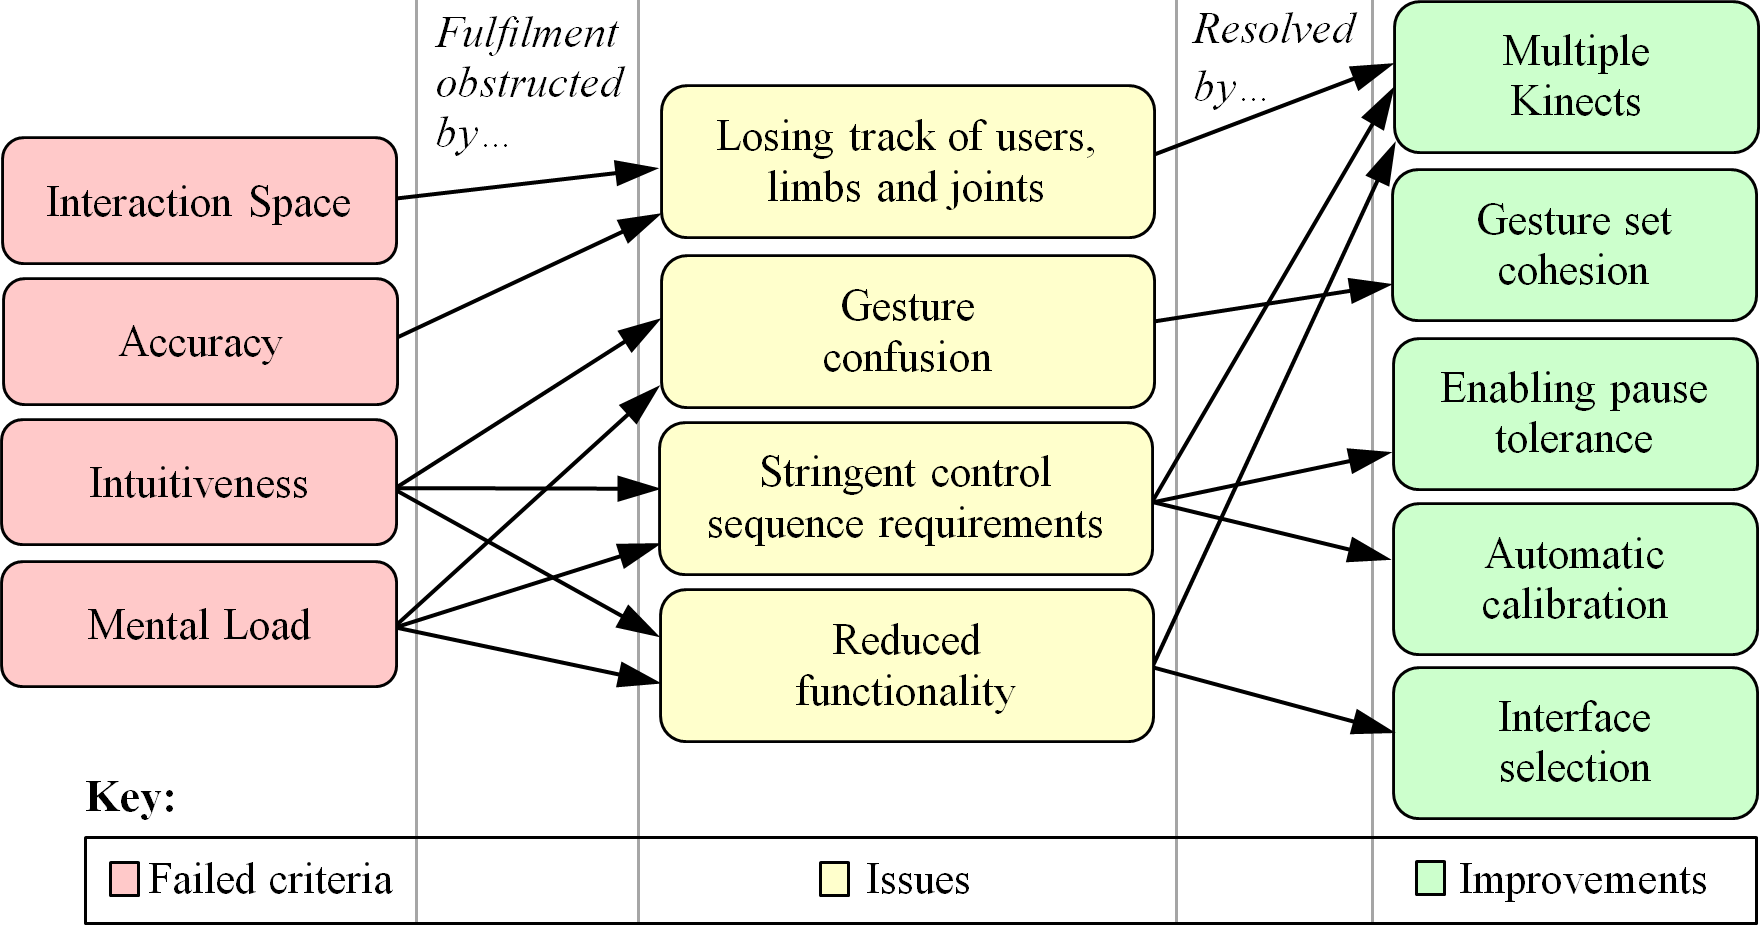
\includegraphics[width=0.5\textwidth]{figures/issue_flow_diagram.png}
  \caption{The connections between failed criteria, observed issues and implemented improvements.}
  \label{fig:issueFlow}
\end{figure}

Figure~\ref{fig:issueFlow} outlines what issues cause the failure of various criteria and the implemented solutions intended to resolve them.

\subsubsection{Multiple Kinects} 
\label{subsubsec:studyImplementationMultipleKinects}

\begin{figure*}[t]
  \centering
  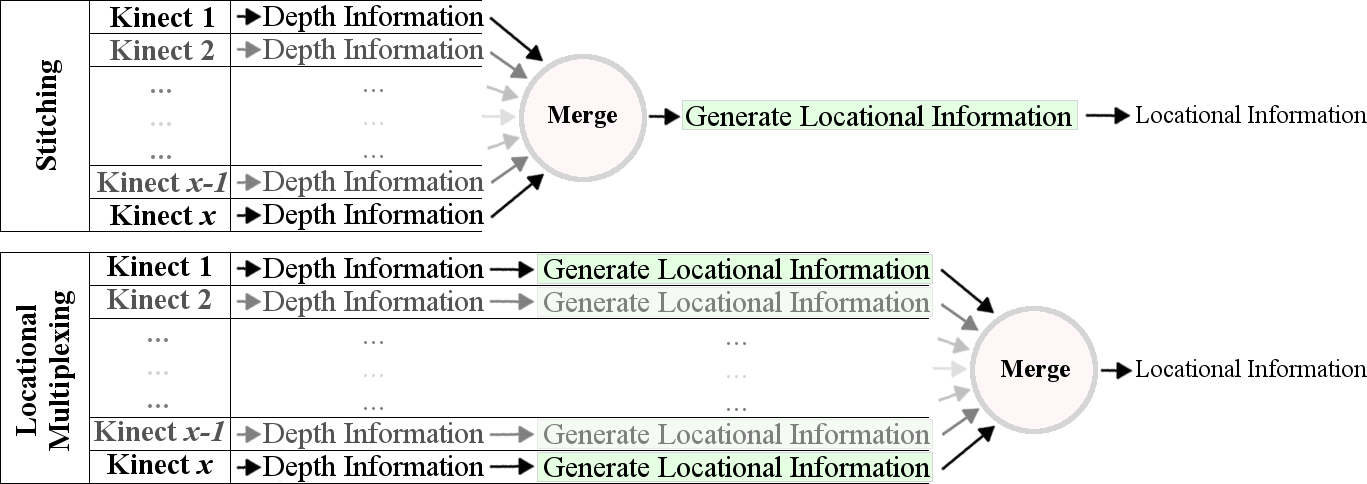
\includegraphics[width=1\textwidth]{figures/multiplexing_flow_diagram.png}
  \caption{The comparison between stitching depth images and multiplexing locational information from multiple Kinect devices.}
  \label{fig:multiplexing}
\end{figure*}

It was decided that the SynergyNet system should be modified to allow for the use of multiple Kinects.
This was the most cost-effective way to improve the system's accuracy.
The use of multiple Kinects may also resolve another limitation of the Kinect.
This is the requirement of users to face the Kinect when performing certain gestures.
This requirement does not render the system unfit for purpose but its resolution is desirable for a more intuitive user experience.
For example, the gesture of hands being held together at the torso requires the teacher to be facing the Kinect when it is performed.
If the teacher is not facing the Kinect their torso will be obscuring the device's view of their hands.
This means the Kinect will not see that the hands are together and will not recognise the gesture.
The use of multiple Kinects should allow the devices to view teachers from multiple perspectives.
This reduces the issue of obstruction and as a consequence, improves the system's ubiquity.
This is due to the teacher being made able to perform gestures at any location in the environment while facing any direction.
The use of multiple Kinects also reduces mental load since the teacher will not need to put as much forethought into positioning themselves so that they are visible to a sensing device.

To avoid the issue of interference, noted in Section~\ref{subsubsec:studyResolvingIssues1} to occur when multiple Kinects are used together, the strategy of placing the devices perpendicular was adopted.
This reduces interference and does not incur any additional cost.
This does, however, reduce the maximum number of Kinect devices which can be used together to two.
This is enough to cover the entire SynergyNet lab but could be problematic for larger classroom.
In addition to cost, several of the alternative solutions were not chosen due to their potential effect of reducing the system's responsiveness.

To combine the information collected from the Kinect devices a multiplexing approach was applied to the positional information collected by the devices.
This was done through taking the user and joint location information from the devices and transforming them to be relative to the environment they exist within.
This results in the locational information from multiple devices being relative to each other.
If two or more locational points supplied by different devices are noted to inhabit the same space the system determines that they are the same user or joint viewed by multiple devices.
The locational information can then be merged into a single entity before being forwarded on.
This ensures that no duplication of locational information takes place and allows the system to identify when the same entity is seen by multiple devices.
This is similar to how touch information from multiple sources can be multiplexed together using the TUIO protocol~\cite{Kaltenbrunner2009}.

Through the use of multiplexing, SynergyNet is capable of tracking a user across the view of multiple Kinects as long as there is some overlap between them.
Overlapping views are made possible through the perpendicular placement of the devices. 
When a teacher passes through the overlapping view the system's multiplexing retrieves the same set of locational information from two devices.
The system then establishes that the sets of locational information are linked to the same entity and merges them into one.
This allows the teacher's identity to be carried over to other Kinect devices.
Therefore, the teacher does not need to re-establish their identity when moving about the classroom environment.
This reduces the amount of teacher interaction required in the control sequence and alleviates mental load. 

The SynergyNet framework consists of different types of node which exist on a network.
Kinects are supported by one type of SynergyNet node whilst student touch-interfaces use another.
A new node was created to support the act of collecting and combing information from multiple Kinect devices.
This node is labelled as the multiplexer.
A single instance of this node is intended to run in the SynergyNet system, collecting information sent out by Kinect nodes.
The multiplexer can then distribute the locational information to the relevant nodes.
The multiplexer node can also share information on which points of locational information from the Kinect devices are the same.
This allows the Kinect nodes to correctly establish identities.
Despite the limitation of only two Kinects devices due to interference, the SynergyNet framework is setup to allow any number of Kinect nodes.

This multiplexing approach was chosen over alternatives, such as stitching the visual and depth views from the devices~\cite{Dubois2011}, due to its minimal processing costs.
The stitching and multiplexing approaches are both similar since they entail identifying information common to multiple devices and using that overlapping data to merge their outputs.
The Kinect device takes complex depth data and turns it into relevant locational information.
Stitching combines the raw depth information whereas multiplexing would entail combining the locational information of user's centre of mass and joints.
Figure~\ref{fig:multiplexing} shows how, when the information from multiple Kinects is merged affects the distribution of processing.

Stitching would require depth information to be merged after being collected by the devices.
This would therefore create a single pipeline from that point onwards where the process of locating users and their joints from the depth information would only need to be applied to a single input.
This modification would increase the interaction space monitored by the system.
This may also result in greater accuracy since the processes used to determine locational information would have a much more detailed input.
A larger input may require more processing power, but with the multiple feeds correctly merged any duplicated information, i.e. from the overlapping areas of the views, would only need to be processed once.
This could reduce the overall processing required.
However, if Kinect devices are being used on separate machines then when following the approach of multiplexing locational information, they can process their captured inputs to generate locational information in parallel.
Processing a single pipeline of depth information would bypass the time-saving benefits of processing the depth information from the devices in parallel.

The stitching approach may require low-level functions provided by the Kinect device's firmware and supporting libraries to be rewritten.
Multiplexing location information can be performed entirely within SynergyNet since it uses the output from the Kinect devices and does not require interrupting their existing processes.

It is also important to note that the amount of depth information collected from the Kinect device occupies much more memory than the locational information it ultimately produces.
The smaller amount of information to be shared for locational multiplexing is beneficial since it must be transmitted through the network.
With more information present when stitching the collected depth values, the process of merging the input from multiple sources is much more expensive computationally than merging the locational information.

The use of multiple Kinects also aides in alleviating the stringent control sequence requirements.
If the teacher can be tracked over a larger area they will leave the system's observed area less frequently.
This reduces how often the teacher would need to re-establish their teacher status with the Kinect node GUI.
In addition to this the use of multiple Kinects will support the implementation of the pointing gesture for interface selection.
With multiple perspectives the teacher's torso cannot obscure where they are pointing.

\subsubsection{Gesture Set Cohesion} 
\label{subsubsec:studyImplementationGestureSet}

To improve the cohesion of the gesture set it was decided that all the upper-body gestures used in the control sequence should conform to an overarching pattern.
As noted in Section~\ref{subsubsec:studyResolvingIssues2}, the most obvious pattern amongst the existing gestures was their similarities to related real-world actions.
It was also noted that several of the gestures in the set did not follow this pattern.
Changing these gestures to ones which bare similarities to related real-world actions may make the gesture set more cohesive.
This should reduce the mental load required by the control sequence since teachers will not need to remember the specific gestures for each command.
If a teacher forgets a gesture they should be able to derive it from a related real-world action.
In addition to this, making the gestures similar to real-world actions may improve their intuitiveness as they act as metaphors~\cite{Wang2008}.

To identify the most suitable new gesture for this action the results from the original guessability study were used.
When ranking gestures by popularity amongst participants in the study, any gestures which do not resemble a related real-world action were discounted.
Two of the gestures in the existing gesture set were identified not to follow the metaphor pattern.

One gesture identified to not follow the metaphor pattern was the holding up of one hand, used to send content to the board.
Holding a hand in the air bares little to no resemblance to any real-world action involving sending or retrieving objects.
Metaphor-based gestures related to the command of sending content to the board should bare resemblance to the similar real-world action of moving items.
The highest ranking metaphor-based gesture for the command of sending content to the board which bares resemblance to a related real-world action was a pushing motion.
Two gestures were more frequently suggested by participants in the guessability study for this command; holding one hand up (previously used) and pointing with both hands.
However, no relation to the action of sending items relate to either of these gestures.
Therefore the gesture of pushing is the most popular metaphor-based action for sending content.
The suitability of the pushing gesture is supported by its resemblance to the pulling gesture used for the related command of retrieving content from the board.

The second gesture identified which did not follow the metaphor pattern was the waving gesture used to gain the Kinect's attention.
While it could be argued that waving is a common action used to gain attention the teacher was noted on several occasions to omit it from the control sequence, resulting in errors.
In addition to this, many of the errors observed in the original study were noted to be caused by the teacher performing this gesture incorrectly.
The wave gesture required users to move their hand left to right twice.
Teachers in the study however were observed to move their hand left to right more than twice, usually continuing until they noticed the Kinect had reacted.
This would have the consequence of causing the hand movements superfluous to the wave being viewed by the system as a different gesture.
Because of this the wave gesture can be seen as problematic.
Changes can be made to the control sequence to make the system more tolerant of errors made performing the wave gesture.
However, it may be more beneficial to replace the gesture with one which bears a strong resemblance to a real-world counterpart.
Using the results from the previous guessability study it is apparent that one of the most popular gestures in the study was the holding of one hand up.
This gesture is now no-longer affiliated with any other commands since the reassignment for sending content to the board.
Holding one hand up is an action common to classrooms for requesting attention.
This is usually performed by the students but its popularity in the guessability study indicates it should be intuitive to the teacher.
Therefore, holding one hand up was chosen to replace waving as a method of gaining the system's attention.

All the gestures used in the framework now bare resemblance to related real-world actions.
The gesture set can be said to be more cohesive with no more outlying gesture which do not conform to the metaphor pattern.

\subsubsection{Enabling Pause Tolerance}  
\label{subsubsec:studyImplementationPauseTolerance}

A pause was implemented into the control sequence at positions before and after identifying a teacher performing a gesture.
These pauses are where the system will ignore any actions performed by the teacher.
This means that the system will ignore the movement of teacher's limbs between gestures, reducing the likelihood of unintentional gestures being performed.
These pauses last one and a half seconds, giving teachers time to move their limbs to the appropriate positions for the next gestures without significantly slowing down the control sequence.

\begin{figure*}[t]
  \centering
  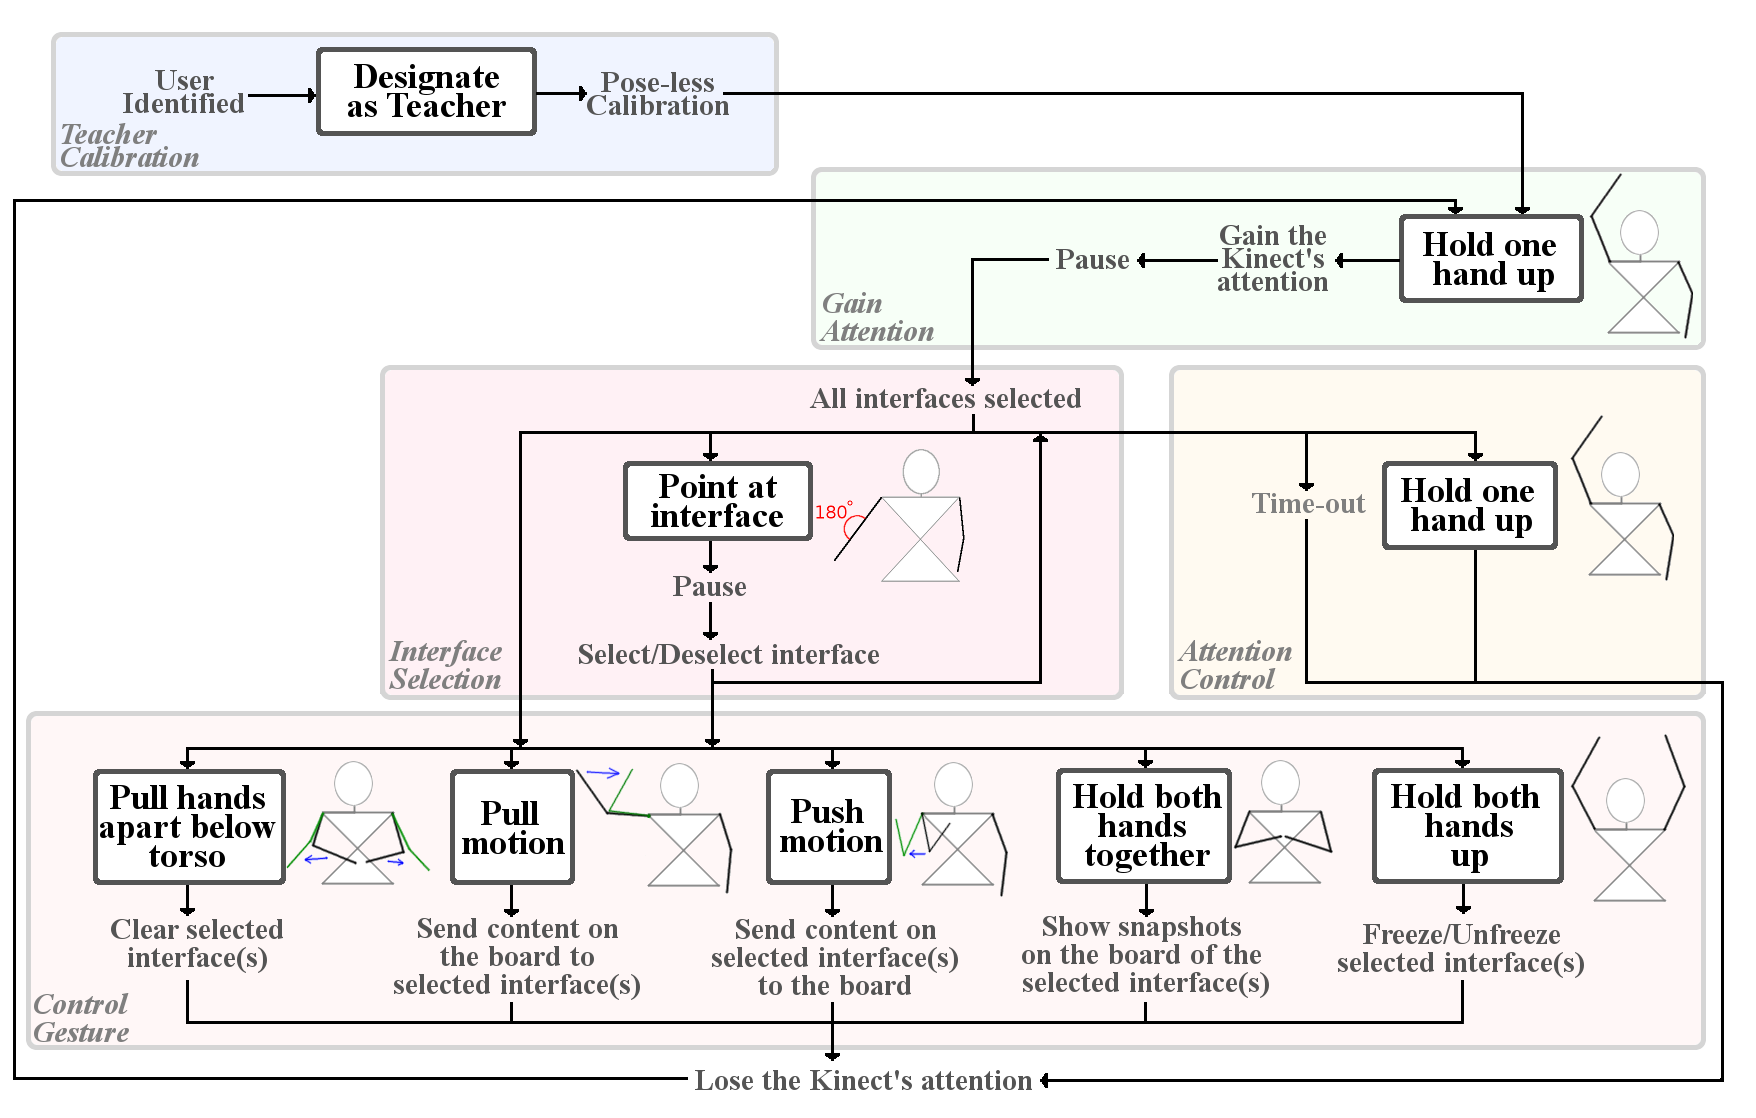
\includegraphics[width=1\textwidth]{figures/control_sequence_flow_diagram.png}
  \caption{The improved control sequence implemented for the gesture controls in SynergyNet.}
  \label{fig:controlSequenceFlowDiagram}
\end{figure*}

\subsubsection{Automatic Calibration}  
\label{subsubsec:studyImplementationAutoCalibration}

The control sequence was also augmented by the implementation of automatic calibration.
With this the teacher does not need to perform a calibration pose for the Kinect to track their upper-body joints.
This reduces the amount of input the teacher needs to provide into the control sequence, thus reducing the mental load required to use the system.
The implementation of automatic calibration is also beneficial for the implementation of multiple Kinects.
Multiple Kinects need the teacher to re-calibrate for each device.
Without automatic calibration the teacher would be required to perform the calibration pose in front of each Kinect before the device could provide meaningful data.
Automatic calibration saves the time and mental load which would be required to repeatedly perform this pose.

\subsubsection{Interface Selection}  
\label{subsubsec:studyImplementationInterfaceSelection}

With the system augmented to use multiple Kinects the teacher should only be able to obscure a single Kinect's view of the interfaces pointed at.
Therefore, the control sequence was augmented to include the pointing gesture for the selection of interfaces.

By pointing at an interface, the teacher can select the specific instances of SynergyNet to be affected.
Teachers can de-select an interface by pointing at it again.
If a teacher performs the command gesture without pointing at any interfaces, the corresponding command will affect all interfaces.

To identify a pointing gesture the Kinect node notes when the angle between a teachers upper and fore-arms at the elbow is close to one hundred and eighty degrees.
This indicates that the arm is being held out straight in a pointing gesture.
If arm is pointing directly down it is ignored because the arm may be at rest.
Likewise, if the arm is pointing upwards it is ignored as there is no scenario where a teacher should need to point up at a table interface in a typical classroom environment.

When a pointing gesture is made, the vector along which the arm points and the location of the pointing hand are captured.
The information is then made relative to instances of SynergyNet running on student interfaces.
The SynergyNet instance can then verify whether a ray fired along the pointing vector from the user's hand would intersect with the interface it is displayed on.
If so, this triggers a selection or de-selection event.

The implementation of the pointing gesture is intended to improve intuitiveness because of its relation to the commonplace real-world action of pointing to identify an object or entity.

The updated control sequence with new gestures and interface selection is summarised in Figure~\ref{fig:controlSequenceFlowDiagram}.

\subsection{Design}
\label{subsec:studyDesign}

% // TODO Trim down - a lot of this is repetition of the first user study section as both were set up and carried out the same way - therefore just mention its the same but discuss the differences (improvements, different class/teacher, etc).

A study was organised to assess the impact of the implemented improvements on the system's use.
The study followed a similar structure to that carried out in previous work.
A primary-school level teacher took part in the study with sixteen of their students.
The teacher was asked to orchestrate four \textit{mysteries} tasks~\cite{AlAgha2010} where students must use clues displayed on the interfaces to answer a question.
For the first three tasks the teacher would use a single control technology; the interactive whiteboard, the tablet or the Kinect, for issuing commands to the student interfaces.
For the final task teachers had all three technologies made available for their use.
The session was recorded using fourteen separate cameras for later data analysis.

The participating teacher was invited into the lab for a day in the week preceding their session.
On this day the teacher was introduced to the control technologies, given a chance to review the tasks to be performed and was allowed to carry out a dry-run of the session.
The teacher was encouraged to \lq think aloud\rq\ throughout the study and announce their intentions before issuing commands through a control technology.
Following the session the teacher was interviewed by the study organisers.

\begin{figure}[h]
  \centering
  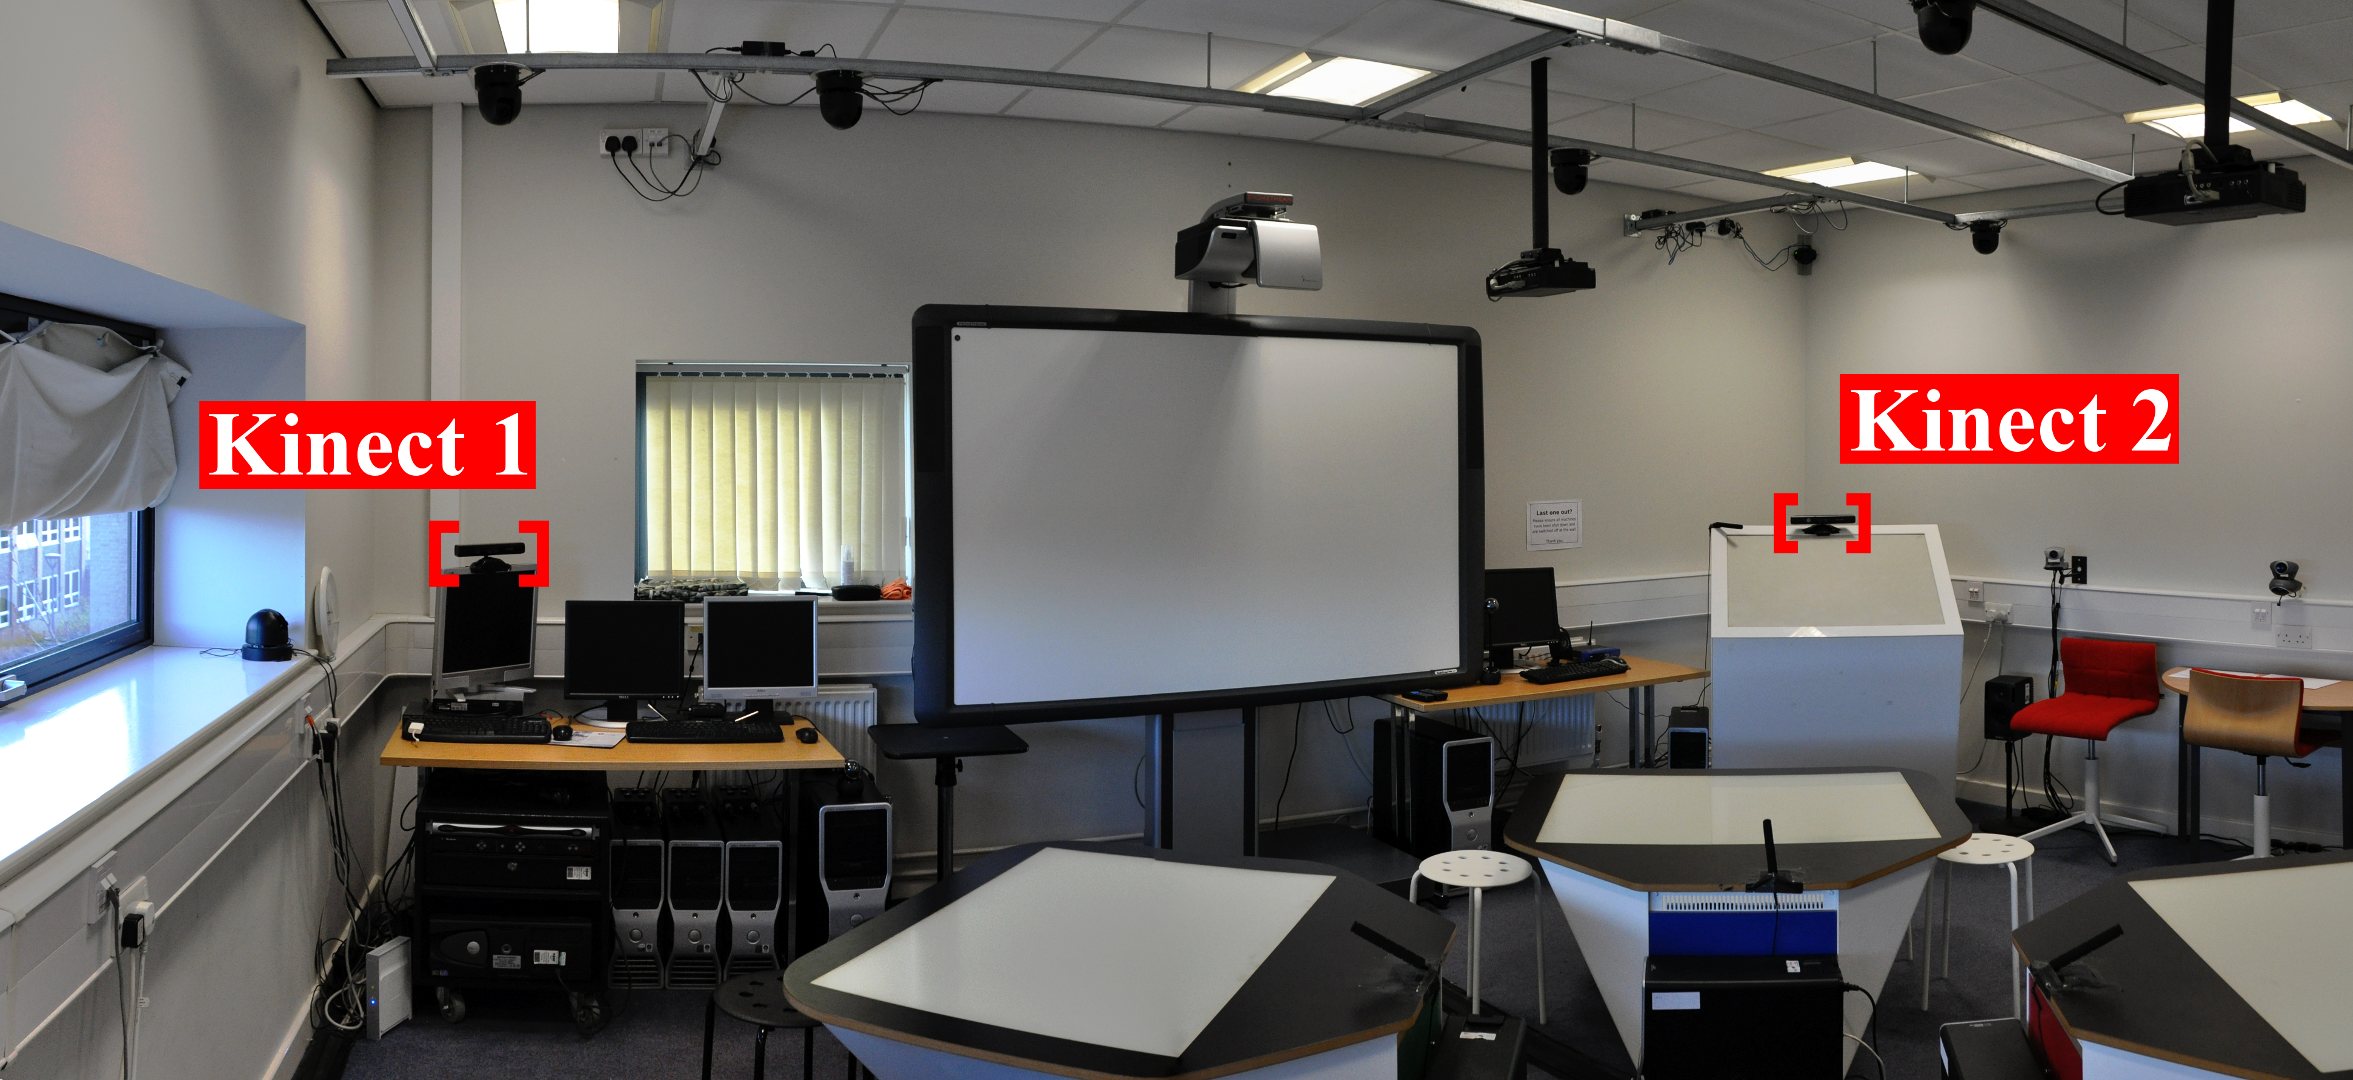
\includegraphics[width=0.45\textwidth]{figures/multiple_kinect_setup.png}
  \caption{The positioning of the two Kinects in the SynergyNet lab during the study.}
  \label{fig:kinectSetup}
\end{figure}

Figure~\ref{fig:kinectSetup} shows the positioning of the Kinect devices during the study.
The devices were place facing perpendicular to each other.
This setup allowed for the entirety of the SynergyNet lab to be observed between the devices.

The primary objective of this study was to assess whether the implemented improvements resolved the issues observed in the previous study.
The study's hypothesis was that the error rate of the Kinects' use would be significantly smaller than the error rate of the Kinect controls in the previous study.

\subsubsection{Data Analysis}
\label{subsec:studyAnalysis}

The criteria used in the previous study, generated from Wachs et al.~\cite{Wachs2011} requirements for hand gestures, was employed to assess the improved upper-body gesture control system.
The success of improvements could be observed through whether previously unmet criteria were fulfilled.

Timing information was collected from the session recordings.
The time from the teacher first announcing their intention to issue a command to the command's broadcast from the controlling technology is classified as the execution time.
The teacher's announcement of their intentions can also be used to identify when the result of the command differs from their intended effect, indicating an error has occurred.

Times taken to perform similar actions with each classroom technology were compared.
In addition to this, the number of errors committed with each technology and quality of communication between the teacher and students were also noted from the recordings.

\section{Results}
\label{sec:results}

% // TODO Trim down.

The study was carried out without any major deviations from its design.
The teacher completed the training for the system the day before the study and stated that they felt confident enough to use the each of the control technologies without any additional aid or practice.

\subsection{Task 1: Board Only}
\label{subsec:resultsTask1}

For task 1 eleven commands were observed to be issued by the teacher in its 19 minute and 43 second duration.
Out of these eleven commands, one was issued incorrectly:

\begin{itemize}
\item This error was observed to occur when the teacher wished to freeze all tables.
When the freeze command was issued two tables were already frozen.
Because the command toggles the frozen state of an instance of SynergyNet, the two tables which were already frozen became unfrozen when the command was issued.
The teacher immediately recognised their mistake and issued a command from the board for specifically freezing the two, now unfrozen, interfaces.
This error was caused by the teacher's understanding of the system's functions and could have occurred with any of the controlling technologies.
\end{itemize}

\begin{figure}[h]
   \centering
   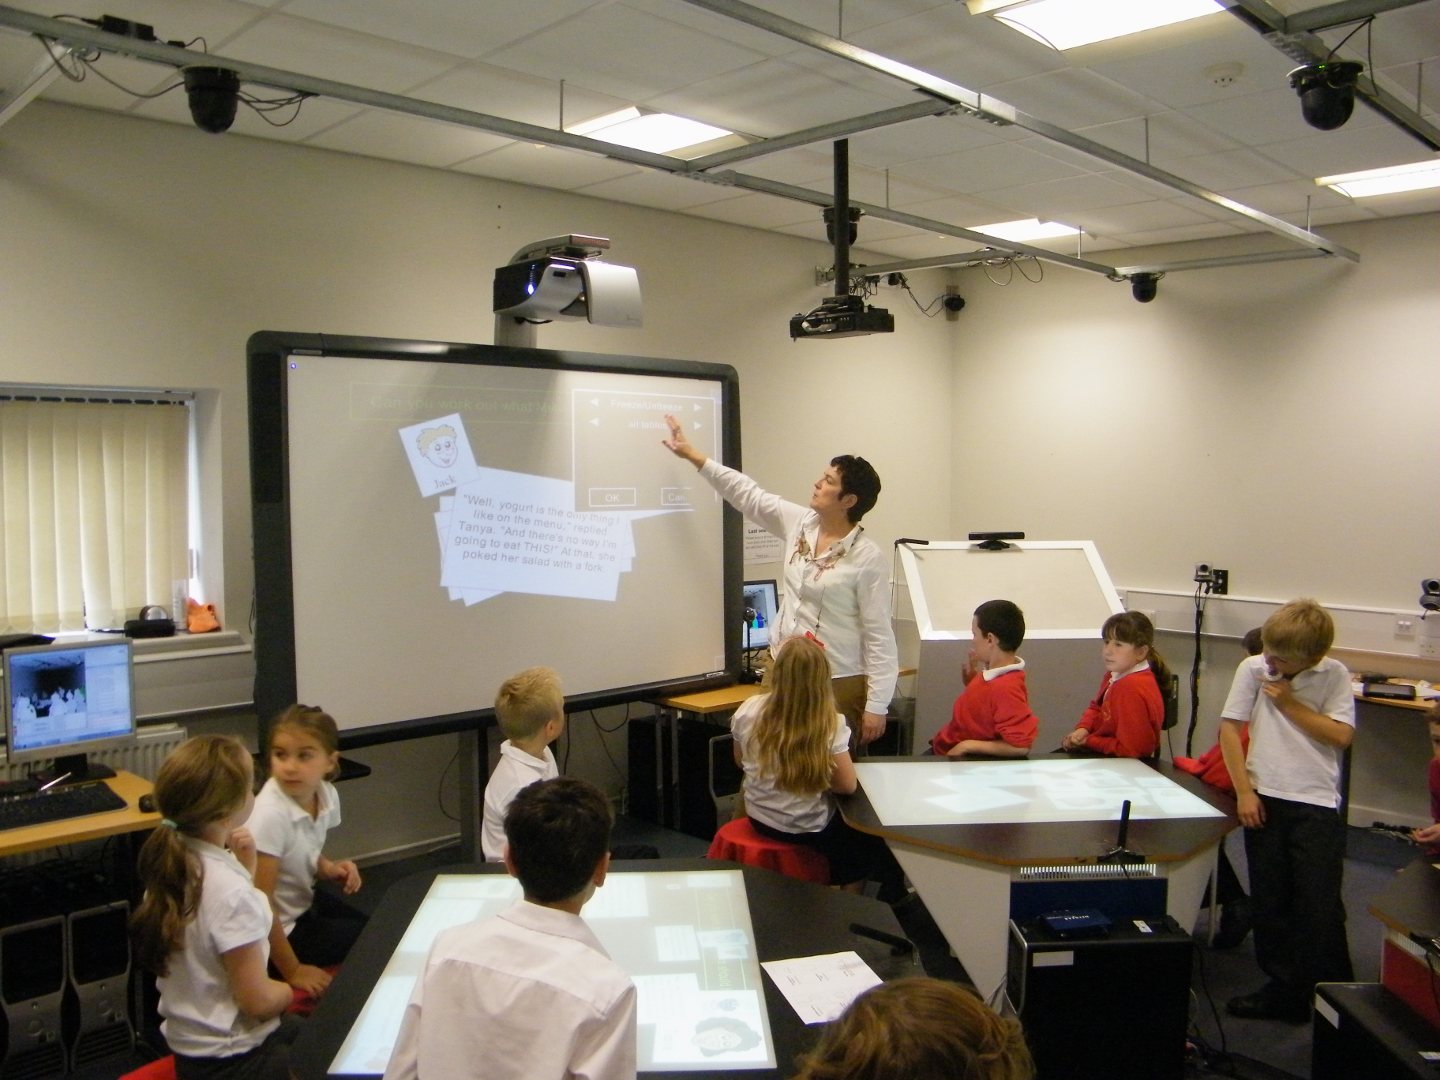
\includegraphics[width=0.45\textwidth]{figures/new_study_board.png}
   \caption{The board control in use during the study.}
   \label{fig:newStudyBoard}
\end{figure}

The average time taken to issue a successful command with the board was 9.82 seconds with a standard deviation of 5.97 seconds.
Six of the successful commands given were intended to affect all student interfaces and four were intended to affect a specific selection.

\subsection{Task 2: Tablet Only}
\label{subsec:resultsTask2}

During task 2, thirteen commands were observed to be issued by the teacher in its 17 minute and 59 second duration.
Of these thirteen commands, three were issued incorrectly.

\begin{itemize}
\item The first of these incorrectly issued commands occurred when the teacher wished to send content from one table to the board.
When this error was made obvious to the teacher by the wrong content appearing on the board they explained to their class that they'd accidentally selected more than one table.
The teacher confirmed this in the post-session interview.
It is apparent that the teacher had left other instances of SynergyNet selected when issuing an earlier command.
The controls accessed through the tablet don't reset the set of selected interfaces when a command is issued unlike the other two control technologies.
The teacher assumed that the tablet controls would behave like the board controls used in the previous study and did not modify their usage accordingly.
This error can be attributed to the tablet's differing behaviour from the board and Kinect controls in regards to interface selection.

\item One of the erroneous commands observed during task 2 occurred when the teacher wished to issue a command to freeze all instances of SynergyNet on the student interfaces.
However, only a selection of the interfaces was frozen.
This was because the teacher did not update the selection criteria.
This is also due to the tablet controls' selection behaviour differing from the alternative technologies'.

\item The remaining error was caused by the teacher issuing a command intended to freeze all interface when several instances of SynergyNet were already frozen.
The outcome of this is that the already frozen SynergyNet instances become unfrozen.
This is a similar occurrence to the single erroneous command observed during task 1.
The teacher assumes that all the interfaces will be put into the same state of being frozen or unfrozen, not toggled from their current state.
This error could occur with any of the control technologies.
\end{itemize}

\begin{figure}[h]
   \centering
   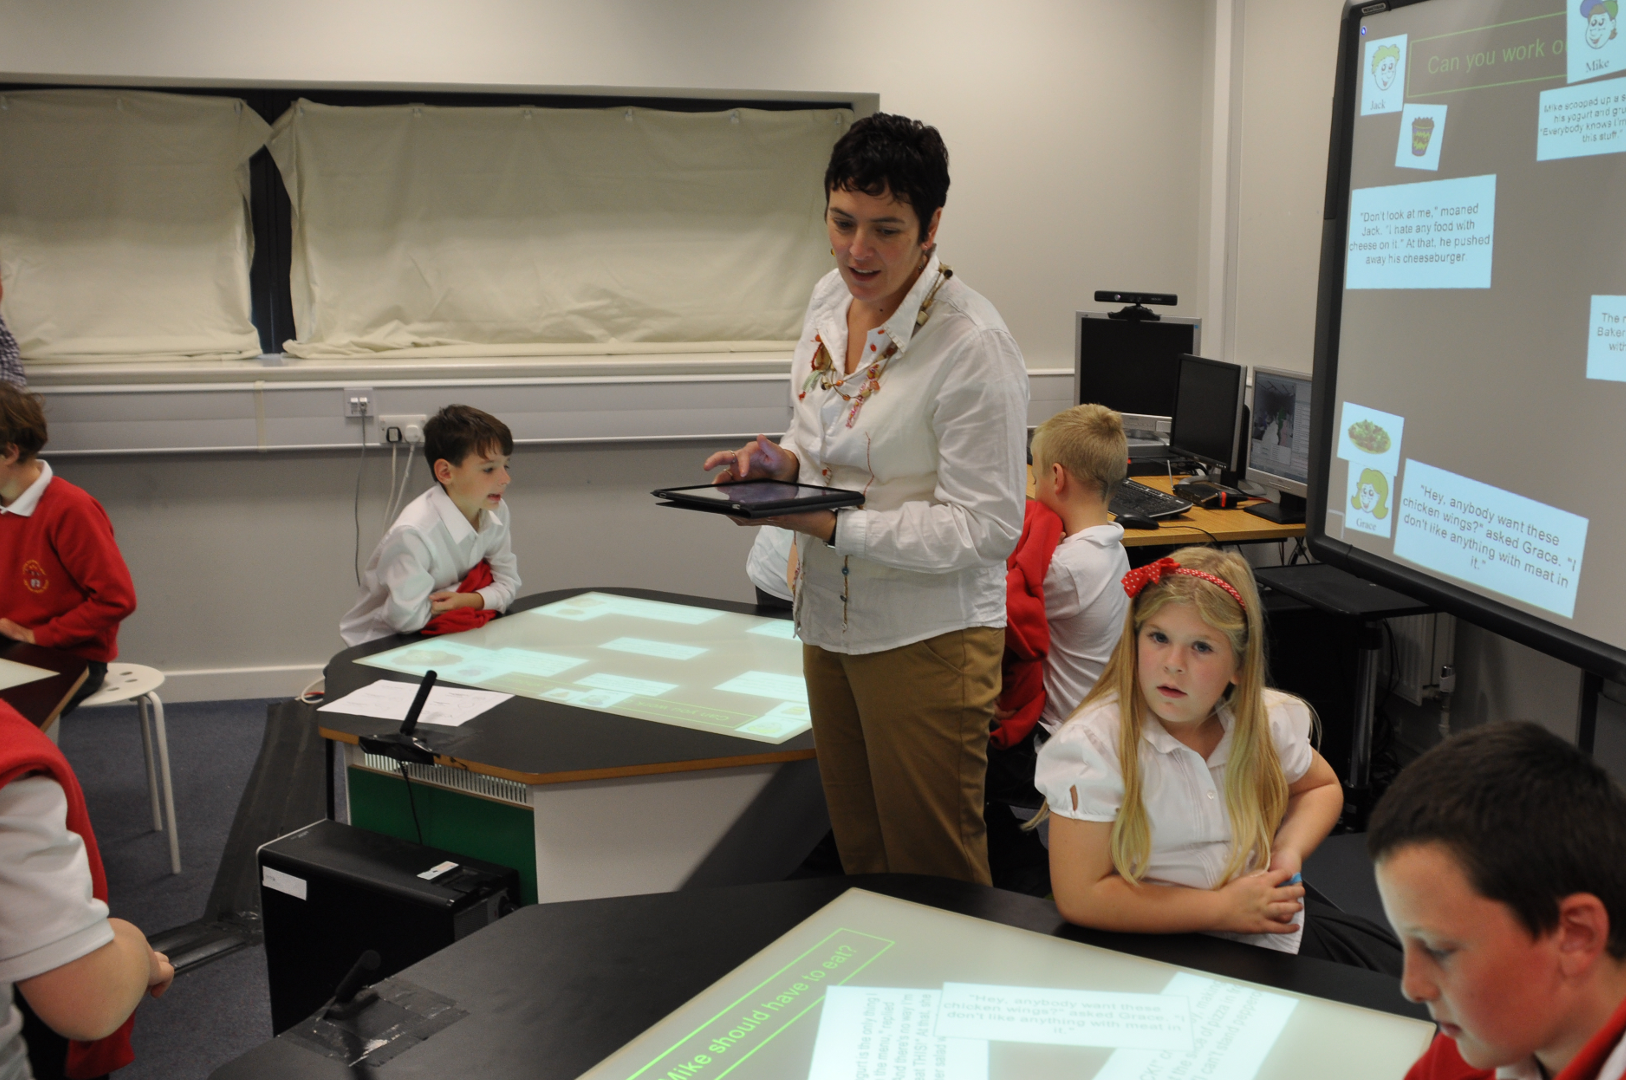
\includegraphics[width=0.45\textwidth]{figures/new_study_tablet.png}
   \caption{The web controls in use during the study, accessed through a tablet interface.}
   \label{fig:newStudyTablet}
\end{figure}

The average time taken to issue a successful command with the tablet was 9.17 seconds with a standard deviation of 13 seconds.
Eight of the successful commands given were intended to affect all student interfaces and two of the successful commands were intended to affect a specific selection.

\subsection{Task 3: Kinect Only}
\label{subsec:resultsTask3}

During task 3, twelve commands were observed to be issued by the teacher in its 18 minute duration.
Of the twelve commands issued during this task with the Kinects, eight were issued with errors.

\begin{itemize}
\item Three of these erroneous commands were observed to occur when the teacher wished to show content from a specific table.
Gaining attention and selecting the table both were problem free for these commands, the error occurred during the control gesture's execution.
To send content to the board the teacher needs to perform a push gesture.
This gesture was not identified by the Kinects and indicates a problem with the device's ability to track these occurrences of the gesture.

\item Two of the erroneous commands in task 3 occurred when the teacher intended to unfreeze all the tables.
The teacher successfully gained the device's attention both times but when they raised both hands for the control gesture the Kinects failed to track one of their arms.
The Kinects only see one arm in the air and interpret the command as the one used to dismiss its attention.
This appears to be a problem caused by the Kinects failing to correctly track the movement of a joint.

\item One of the commands which was issued with errors occurred when the teacher wished to transfer the content on the board to all the tables.
The teacher performed the pull gesture but did not perform the attention gaining gesture beforehand.
This meant that the Kinects ignored the teacher's command gesture.
This error occurred due to the teacher not following the control sequence.

\item Another of the erroneous commands was also observed to occur when the teacher intended to transfer content on the board to all of the student interfaces.
After successfully getting the Kinect's attention the teacher performs the pull gesture.
The Kinects did not see this movement correctly.
The teacher repeated the gesture several times but neither of the Kinects correctly tracked the movement of the hand before their attention timed out.
Instead, the Kinects would often assume that the moving arm was at rest by the teacher's side - a sign that the devices had lost track of the hand and arm joints.
This is another instance of a command made erroneous by the Kinects failing to track a joint accurately.

\item The final erroneous command occurred when the teacher intended to freeze all the student interfaces.
The teacher successfully gained the attention of the Kinect devices then stopped.
In the post-session interview the teacher revealed this was because they were trying to recall the control gesture because they had forgotten it.
The teacher did not resume the control sequence until after the Kinect nodes' attention timed out.
This error occurred due to the teacher not following the control sequence by pausing too long.
\end{itemize}

\begin{figure}[h]
   \centering
   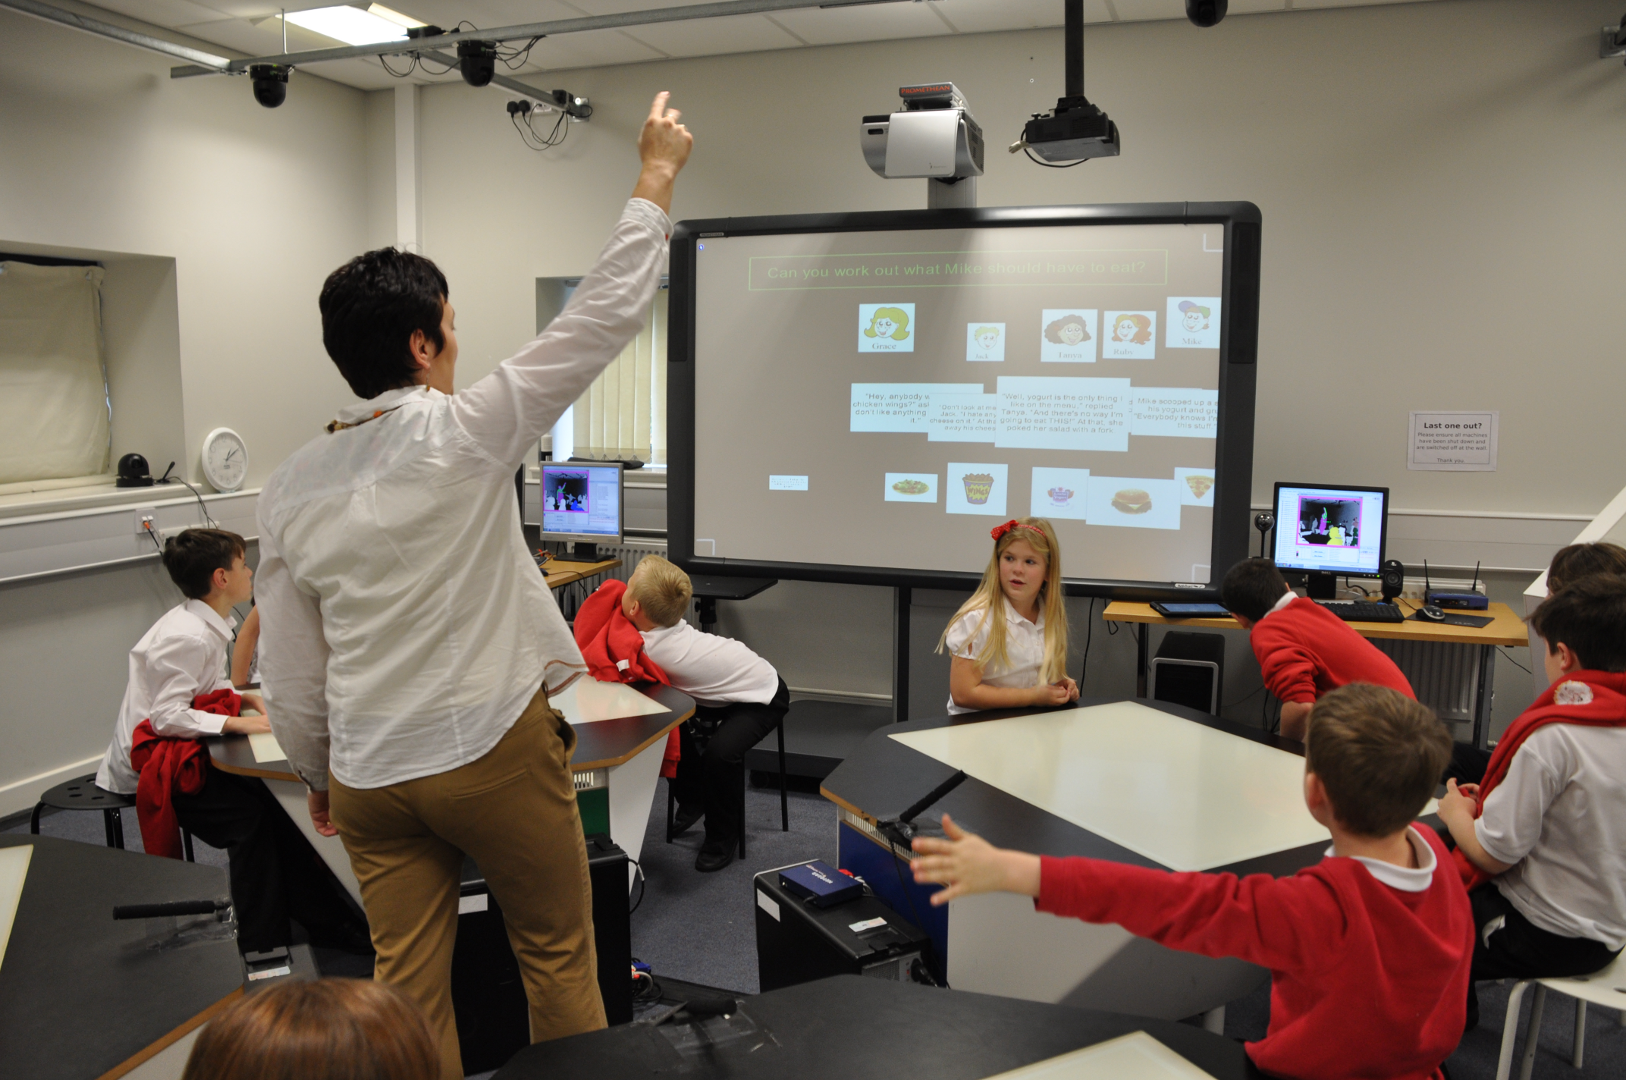
\includegraphics[width=0.45\textwidth]{figures/new_study_kinect.png}
   \caption{The Kinect control in use during the study.}
   \label{fig:newStudyKinect}
\end{figure}

The average time taken to issue a successful command with the Kinects was 2.44 seconds with a standard deviation of 0.54 seconds.
All four of the successful commands were intended to affect all the student interfaces.

\subsection{Task 4}
\label{subsec:resultsTask4}

For task 4, where the teacher had the option of using any of the three control devices, twenty three commands were observed to be issued by the teacher in its 19 minute and 28 second duration.
Nine of these commands were issued through the board control, none through the tablet and fourteen through the Kinects.
Out of these twenty three commands, five were issued incorrectly.
All five of these erroneous commands were issued using the Kinects.

\begin{itemize}
\item Two of the erroneous commands observed in task 4 occurred when the teacher attempted to display screenshots of all the student interfaces on the board.
The Kinects' attention was gained successfully but the devices both lost track of the teacher's right hand when the command gesture of holding two hands together was performed.
Like a number of erroneous commands observed during task 3, this failure to successfully identify a command gesture appears to result from the Kinects' joint tracking abilities.

\item One of the failures to successfully to issue a command occurred when the teacher intended to send content on the board to all tables.
After successfully obtaining the Kinects' attention the teacher performed the pulling gesture.
However, neither of Kinects was able to successfully interpret the movement of the hand as a command gesture.
The Kinects would show the arm moving to a resting position by the teacher's torso part way through the gesture, indicating that both of the devices had lost track of the hand and arm joints.
Again, this is an error caused by the Kinects' joint tracking.

\item Another of the erroneous commands observed during task 4 occurred when the teacher intended to freeze all the student interfaces.
The teacher successfully gained the devices' attention then performed the gesture of holding both hands up.
However, during the command gesture both the Kinects lost track of one of the teacher's hands, placing their left arm in a resting posting.
This had the consequence of only one arm being identified as in the air which was interpreted as the attention dismissing gesture.
This resulted in the teacher losing the Kinect's attention with no command being issued to the student interfaces.
This is yet another instance of the Kinect devices' tracking abilities causing errors.

\item The remaining erroneous command occurred when the teacher intended to send content from a specific table to the board.
After successfully gaining the attention of the Kinects the teacher performed the push command gesture.
Part way through the gesture the Kinects both interpreted the arm of the gesturing hand moving to a resting position.
This indicated that the Kinects had both lost track of the gesturing hand.
This is, again, an instance of the Kinects' tracking abilities causing a correctly performed command gesture to return erroneous results.
\end{itemize}

The average time taken to issue a successful command was 6.73 seconds with the board and 2.81 seconds with the Kinects.
The standard deviation was 3.29 seconds for the board and 1.51 seconds for the Kinects.
Seven of the successful commands given with the board were intended to affect all student interfaces and two of the successful board commands were intended to affect a specific selection.
For the Kinects, four of the successful commands given were intended to affect all student interfaces and five were intended to affect a specific selection.

\subsection{Results Summary}
\label{subsec:resultsSummary}

The usage of the three control technologies in the study is summarised in Table~\ref{table:results2}.

\begin{table}[h]
\centering
\begin{tabular}{!{\vrule width 1.5pt}c|c|c|c!{\vrule width 1.5pt}}
\noalign{\hrule height 1.5pt}
\multicolumn{1}{!{\vrule width 1.5pt}c!{\vrule width 1.5pt}}{\textbf{}}	
&\textbf{Number}
&\multicolumn{1}{!{\vrule width 1.5pt}c!{\vrule width 1.5pt}}{\textbf{Number}}	
&\textbf{Avg. time}\\
\multicolumn{1}{!{\vrule width 1.5pt}c!{\vrule width 1.5pt}}{\textbf{}}	
&\textbf{of}
&\multicolumn{1}{!{\vrule width 1.5pt}c!{\vrule width 1.5pt}}{\textbf{of}}	
&\textbf{to issue}\\
\multicolumn{1}{!{\vrule width 1.5pt}c!{\vrule width 1.5pt}}{\textbf{Device}}	
&\textbf{commands}
&\multicolumn{1}{!{\vrule width 1.5pt}c!{\vrule width 1.5pt}}{\textbf{errors}}	
&\textbf{commands}\\
\noalign{\hrule height 1.5pt}
Board 					&20 					&1				&8.28 seconds				\\
\cline{1-4}
Tablet 					&13					&3				&9.17 seconds				\\
\cline{1-4}
Kinect 					&26					&13			&2.63 seconds				\\
\noalign{\hrule height 1.5pt}
\end{tabular}
\caption{The usage of the control devices in the study.}
\label{table:results2}
\end{table}

The results show that the Kinect was the much faster control technology for issuing commands but also had the highest error rate.
Though the error rate is smaller than that in present in the previous study, its magnitude indicates that not all the issues intended to be countered by the implemented improvement have been resolved.

\section{Discussion}
\label{sec:discussion}

% // TODO Trim down.

In the previous study the Kinect controls had an overall error rate of 86.96\meaning that twenty in twenty three commands were erroneous.
As Figure~\ref{fig:controlDevicesErrors} shows, the error rate for the Kinect controls in this study was 50\%.
This equates to one in two commands being erroneous.
This is a great improvement over the previous study's error rate and indicates that the hypothesis of a significantly reduced error rate given in Section~\ref{sec:results} was correct.

\begin{figure}[h]
  \centering
  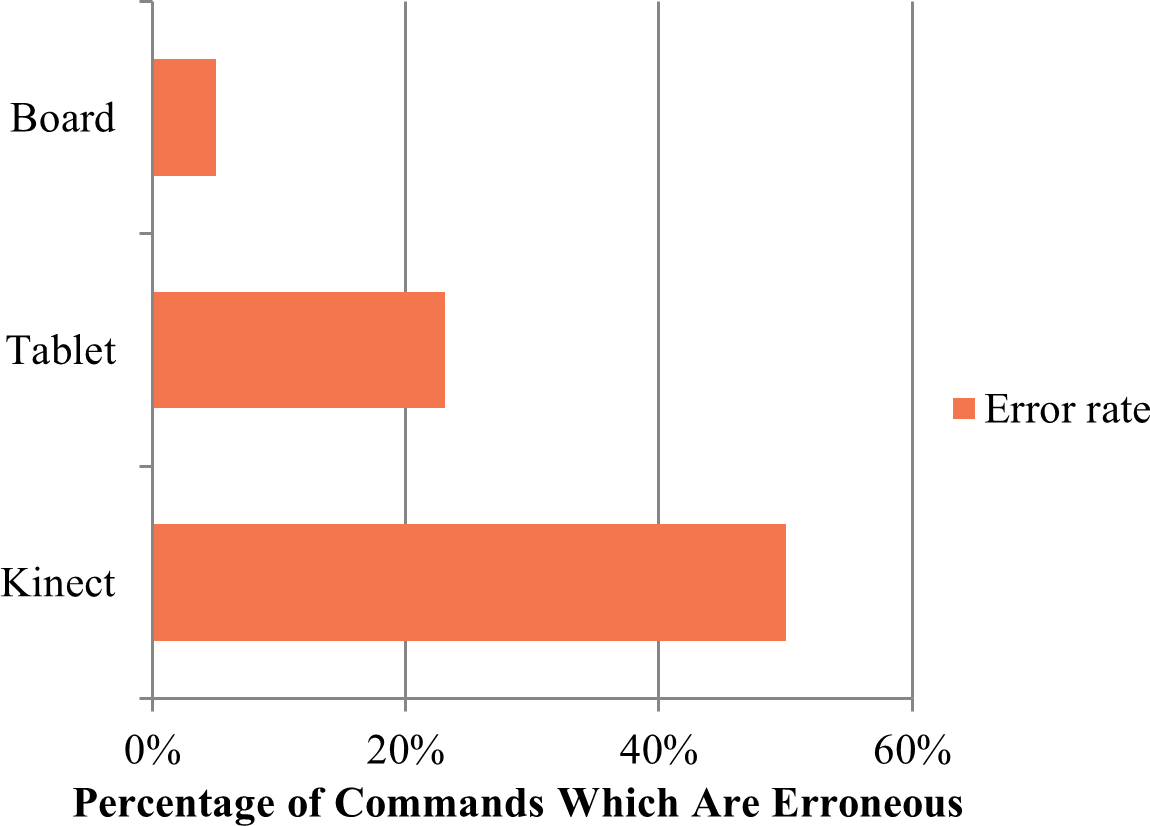
\includegraphics[width=0.45\textwidth]{figures/bar_chart_errors.png}
  \caption{Comparison between the error rates of each of the control technologies.}
  \label{fig:controlDevicesErrors}
\end{figure}

The results indicate that the implemented did have a positive impact on the system but the impact was not as great as intended.

\subsection{Successfulness of the Improvements}
\label{sec:discussionSuccess}

The 50\% error rate indicates that there are still issues with the system and that a selection of the improvements may have had little to no positive consequences.

\subsubsection{Multiple Kinects}
\label{sec:discussionSuccessMultipleKinects}

The implementation of multiple Kinect increased the monitored range of the system.
Throughout the entire study, the teacher never needed to re-establish their teacher status after the initial setup.
This saved a great amount of time in comparison to the previous study where the teacher needed to repeatedly re-establish their teacher identity and perform the calibration pose.
In addition to this, the reduction in teacher input required by the Kinect control indicates a simpler control sequence which aids intuitiveness and mental load.

Despite these improvements, the majority of errors observed in the study originated from the Kinect devices themselves.
Eleven of the thirteen unsuccessful commands executed with the Kinect controls were made erroneous due to the Kinect devices losing track of a joint.
This indicates that the intended effect of improving the devices' accuracy through the use of multiple Kinects did not come to fruition.
Though the use of multiple Kinects did improve the system's Interaction space, functionality and speed of use, they did not fulfil their intended purpose of reducing errors relating to accuracy to a satisfiable level.

\subsubsection{Cohesive Gesture Set}
\label{sec:discussionSuccessCohesiveGestureSet}

The implementation of a more cohesive gesture set appears to have been a successful improvement to the system.
The results of the study show that the teacher never confused any of the gestures.
In addition to this the teacher rarely had any problems recalling a specific command, only once pausing for a significant amount of time to recall one.
This was during task 3 when the teacher wished to freeze all the student interfaces.
This appeared to be a temporary lapse in memory since the teacher had performed the same gesture several times before and after this occurrence.
The more cohesive gesture set seems to have been successful as no errors relating to gesture confusion were observed to occur during the study.

\subsubsection{Pause Tolerance}
\label{sec:discussionSuccessPauseTolerance}

Enabling pause tolerance in the control sequence appears to have improved the system.
The frequency of errors caused through the system wrongly identifying the movement of teachers between stages of the control sequence as command gestures appears was reduced in comparison to the previous study.
Only one erroneous command resulted from a teacher's movements between stages of the control sequence.
This was when the teacher paused while trying to recall the command gesture after getting the Kinect devices' attention.
This pause was much longer than the system anticipated and its attention timed out.
However, the teacher when realising their mistake simply repeated the control sequence again without pausing for so long and successfully issued the desired command.
The implementation of a tolerance for teacher pauses appears to have been successful, though it could benefit from allowing longer pauses between actions.

\subsubsection{AutomaticCalibration}
\label{sec:discussionSuccessAutomaticCalibration}

Implementing automatic calibration appears to have had its intended effect of simplifying the control sequence to aid intuitiveness and mental load requirements.
The teacher never needed to perform the calibration pose, saving time and reducing the amount of teacher input required by the system.
This simplification of the control sequence may have resulted in the teacher only once performing the steps needed to issue a command incorrectly.
The teacher during task 3 intended to send content on the board to all the student interface but performed the command gesture before getting the Kinect devices' attention.
This was a one off error and because it was the first command attempted with the Kinect devices in the study could be attributed to being an insignificant mistake.
The results indicate that the implemented improvement of automatic calibration was successful.

\subsubsection{InterfaceSelection}
\label{sec:discussionSuccessInterfaceSelection}

The implemented improvement of interface selection had its intended effect of enabling a teacher to select which tables a command would affect.
This gave the Kinect controls the same functionality as the alternative control technologies.
There were no errors observed during the table selection phase of all the commands issued throughout the study.

Though interface was never used in task 3, its use in task 4 indicated that its use was of great benefit.
Of the nine successful commands issued during task 4, five of the commands were issued using interface selection.
This was a greater share of the commands than the two intended for specific interface issued from the board controls during the same task.
This indicates that the teacher not only had no problems in using the interface selection on the Kinect, but they also preferred it to the interface selection functionality in the other control technologies.
This was confirmed in the post session interview where the teacher stated their preference for the Kinect, specifically the interface selection stage.
The teacher mentioned that the tablet control's interface selection caused all of the errors observed in task 2.
The fear of repeating the same errors was the reason given by the teacher for not using the tablet controls at all during task 4.

The table interfaces in the SynergyNet classroom use unique colours for identification.
The board and tablet controls used the table colours to identify the specific instances of SynergyNet a command may affect.
The teacher stated that interface selection with the board controls was problematic as they would have to turn and check the colour of the interface they wished to select.
With the Kinect's interface selection the teacher would point directly at the intended interface.
This more direct selection method simplifies the interface selection process and aids in intuitiveness and mental load alleviation.
The implementation of interface selection not only allowed the Kinects to match the functionality of the other control technologies but was also preferable to the alternative controls' interface selection.

The results demonstrate that the interface selection implementation was successful in improving the functionality of the Kinect controls.

\subsection{Resolution of the Issues}
\label{sec:discussionResolution}

The distribution of erroneous commands across the improvements indicates that implemented improvements have been successful in resolving the majority of issues noted in the previous study.
The Kinect controls' 50\% error rate observed during this study are therefore caused by the minority of issues that remain unresolved.

\subsubsection{Losing Track of Users, Limbs and Joints}
\label{sec:discussionResolutionLosingTrack}

The issue of the Kinect devices losing track of user's limbs and joints remains a significant source of errors despite the implemented improvements.
Despite the use of multiple Kinects proving beneficial to other implemented improvements, such as interface selection, it has not improved the system's accuracy.
Of the thirteen erroneous commands issued with the Kinect observed to occur in the study, the failure of eleven of these commands was attributed to the devices losing track of users' joints.

All occurrences where the Kinect devices lost track of a user's limbs and joints were observed to occur when the teacher's body was entirely within the device's range.
This indicates that limited interaction space was not the cause of the tracking problems.
No erroneous commands in the study were observed to occur due to the teacher's limbs and joints leaving the devices' observed area.
This indicates that the system's interaction space is sufficient.

Though the range of the system's observed area is greater the devices still appear to have issues with tracking the movement of user's limbs.
It appears the Kinect has issues which tracking the movement of the teacher's arms during specific gestures.
The majority of the gestures affected appeared to be those which required the movement of a hand.
This indicates that the Kinect may have issues with tracking movement of limbs.
It is possible that the Kinect may not be responsive enough to accurately track the movement of teacher's hand performing gestures such as push and pull.

Another cause for the inaccurate tracking could be occlusion~\cite{Meng2012}.
Movement by the teacher during a gesture may momentarily obscure the tracked joints from the Kinect's view.
While a joint is momentarily obscured from view the Kinect may assume it has taken to a resting position.
This was observed to occur several times during the study.
This movement of an arm mid gesture to a resting position changes the gesture's perceived movement in such a way that SynergyNet will not recognise the gesture.
Though two Kinects observe each gesture, a brief occlusion of the tracked joints on both systems during the teacher's movement (not necessarily at the same time) will break their recognition of the gesture.

However, there were some gestures where the teacher holds a pose, such as holding two hands in the air to issue the freeze command, during which the Kinect lost track of a hand joint.
It is possible that while the teacher moved their arms from the attention getting gesture to the command gesture that the Kinect's lost track of the arm joints due to the speed of the arms movement or momentary occlusion.
Both the observing devices may not have been able to re-establish the location of the hands once they were held in place since the Kinect uses the movement of users to track their joints.
Another possibility is that though the hand joints were within range of the Kinect they may have occupied the inaccurate regions near the edges of the devices' views~\cite{Mehrotra2011}.
Since the hands were held in the air this could be due to their proximity to the top of both the Kinect device's views.
This inaccurate area could account for why both the Kinects' lost track of one of the arms, observed from footage of the study to be the one held higher, and assumed it to be at rest.

These observations on the failings of the Kinect to track the teacher's arms that despite the improvement, the device still has issues with accurately tracking joints.
The implementation of multiple Kinects is not capable of resolving this issue.

\subsubsection{Gesture Confusion}
\label{sec:discussionResolutionGestureConfusion}

The results imply that the issue of gesture confusion observed during the previous study have been resolved.
No instances of erroneous commands due to the teacher performing the wrong gesture were present in the new study.
This indicates that the implemented improvement of a more cohesive gesture set has been successful.

\subsubsection{Stringent Control Sequence Requirements}
\label{sec:discussionResolutionStringentControlSequenceRequirements}

Two erroneous commands were observed during the study which could be attributed to the issue of the stringent control sequence requirements.
These both occurred in task 3.
The first took place when the teacher forgot to gain the Kinect devices' attention and the second happened when the teacher paused for too long before executing a command gesture.
The impact of both these erroneous commands was small since both errors were immediately recognised by the teacher and rectified.

Only two of the thirteen erroneous commands were caused by the issues of stringent control sequence requirements
This means that 15\% of the errors committed with the Kinect resulted from this issue.
This is a much lower share of the erroneous commands than in the previous study where the stringent control sequence requirements accounted for 55\% of the errors committed with the Kinect.
This implies that the use of multiple Kinects, pause tolerance and automatic calibration have succeeded in improving the system's resolving of this issue.
However, the results also show that further improvements could be made to help resolve this issue more effectively, such as allowing for longer pauses.

\subsubsection{Reduced Functionality}
\label{sec:discussionResolutionReducedFunctionality}
 
The results imply that the issue of reduced functionality has been resolved.
The Kinect controls now have the same functionality as the other control technologies and were observed during the study to be the cause of no errors.
The teacher used the selection stage of the Kinect controls on several occasions to issue commands affecting only specific interfaces.
The majority of these commands were successful and when these commands failed it was due to the Kinect's accuracy causing a failure in identifying the command gesture, not the interface selection stage.
The use of multiple Kinects and implementation of interface selection have both allowed the system to resolve the issue of reduced functionality.

\subsection{Fulfilment of Criteria}
\label{subsec:discussionFulfilment}

To assess the success of the improvements in resolving the issues the criteria for evaluation upper-body gestures, derived from Wachs et al.'s~\cite{Wachs2011} requirements can be employed.
If all the criteria are fulfilled the improvements can be said to have been completely successful.
However, with a 50\% error rate this is cannot be determined to be true.
Though not completely successful the results indicate that the improvements have had some positive impact on the system.
This impact may result in system now fulfilling some of the criteria that it previously failed on.
Since all the errors observed during the study originated from issues present in the previous incarnation of the system, no new types of issue can be said to have arisen because of the improvements.
This indicates that the previously fulfilled criteria remain fulfilled.
The system with its improvements can be said to meet the criteria for; cost, adaptability, un-encumbering nature, responsiveness, lexicon size, comfort, interaction space requirement and ubiquity.

\subsubsection{Accuracy}
\label{sec:discussionResolutionAccuracy}

The previous unfulfilled criterion of accuracy cannot said to have been fulfilled by the implemented improvements.
Though the use of multiple Kinects was intended to aid in fulfilling this criterion the Kinect's inaccuracy could be deemed the cause of the majority of erroneous command observed during the study.
The failure to fulfil this criterion is due to the issue still prevalent in the system of the Kinect losing track of user's joints.

The use of multiple Kinects did improve the range of the devices and as a result the Kinect's tracking of users was improved.
Throughout the study the system never lost track of the teacher.
This is evident due to the fact that the teacher was never required to re-establish their teacher status after the initial setup.
This indicates that the Kinect's user tracking accuracy was improved.
However, for this system the Kinect's limb tracking is of much greater use.
The inability to accurately track the teacher's limbs accurately caused the majority of errors observed during the study, specifically 85\% of erroneous errors were caused by the Kinect's inaccurate limb tracking.
The amount of errors and the magnitude of their impact, resulting in eleven commands to be repeated, made the system unfit for purpose.
Therefore, the criterion of accuracy remains unfulfilled by the system.

\subsubsection{Interaction Space}
\label{sec:discussionResolutionInteractionSpace}

Though the implementation of multiple Kinects failed to fulfil the criterion for accuracy, their implementation has been successful in giving the system sufficient interaction space.
None of the erroneous commands which occurred in the study were noted to have been caused by the teacher's limbs or joints leaving the devices' monitored areas.
This indicates that the system's interaction space was improved vastly in comparison to the previous study where the movement of teacher limbs outside the observed area caused many gestures to fail.

\subsubsection{Intuitiveness}
\label{sec:discussionResolutionIntuitiveness}

The teacher was noted in the training session to quickly understand the Kinect control system's use.
During the study the teacher was able to correctly recall the correct gestures and steps of the control sequence quickly and with little forethought for the majority of commands issued.
This indicates that the system's intuitiveness was improved in comparison to the previous study where the teacher's execution of commands was slower and more error-prone.

No major errors relating to intuitiveness appeared during the study.
The two erroneous commands caused by the issues of the stringent control sequence requirements could be said to be related to intuitiveness.
However, the minor impact and infrequency of these errors did not result in the system being made unfit for purpose.
The issues of gesture confusion, stringent control sequence requirement and reduced functionality previously contributed to the system failing to meet the criterion for intuitiveness.
With no majors errors emanating from any of these issues the criterion of intuitiveness could now be said to be fulfilled by the system.

\subsubsection{Mental Load}
\label{sec:discussionResolutionMentalLoad}

The required amount of mental load appeared to be alleviated with the improvements in comparison to the previous study.

In the previous study six erroneous commands were caused by the teacher pausing during the command sequence to think.
In the new study only one error was identified to have occurred due to the teacher pausing.
However, the reduction of these types of errors may be due to the system being made more tolerant of pauses.
Teachers issued commands with the Kinect 60\% faster than in the previous study.
This indicates thinking time was reduced implying a reduction of mental load.

The simplification of the control sequence reduced the amount of input required from the teacher.
Even with the addition of the interface selection stage the teacher was required to provide fewer inputs per command with the improvements.
This was in part due to less frequent repeating of gestures to correct an erroneous command, a benefit of the lower error rate.
In addition to this, there was no need to perform calibration or repeatedly establish teacher status thanks to the improvements.
This reduction in required user input simplifies the user of the Kinect controls and aids in alleviating the mental load required by the system.

The system failing to meet the criterion for mental load in the previous study was caused by the issues of gesture confusion, stringent control sequence requirement and reduced functionality.
The criterion of mental load could now be said to be fulfilled by the system with no major errors emanating from any of these issues.

\section{Conclusions}
\label{sec:conclusions}

% // TODO Trim down.

% Summarise stuff overall (i.e. both phases)

The study was designed to identify whether the implemented improvements detailed in this paper resolved the issues noted to cause the previous implementation of the system to fail to meet certain criteria.
The results of the study reveal that all but one of the criteria were filled by the improvements.
The previously unmet criteria fulfilled by the improvements were those for interaction space, intuitiveness and mental load.
The unmet criterion was the accuracy of the tracking device.
Despite the improvements intended to resolve issues relating to this criterion the accuracy of the tracking devices resulted in the system being unfit for purpose.
This does not mean that the improvements intended to resolve the issues relating to accuracy, i.e. the use of multiple Kinects, were a complete failure.
The accuracy of the system did improve but not enough for the errors it caused to be deemed minor.
In addition to this the use of multiple Kinects intended primarily to improve accuracy aided the resolution of other errors such as the lack of interface selection and simplifying of the control sequence.

The error rate of 50\% was observed to be an improvement on that found in the previous study, 86.96\%.
However, this rate of error is still too high to be considered acceptable.

\begin{figure}[h]
  \centering
  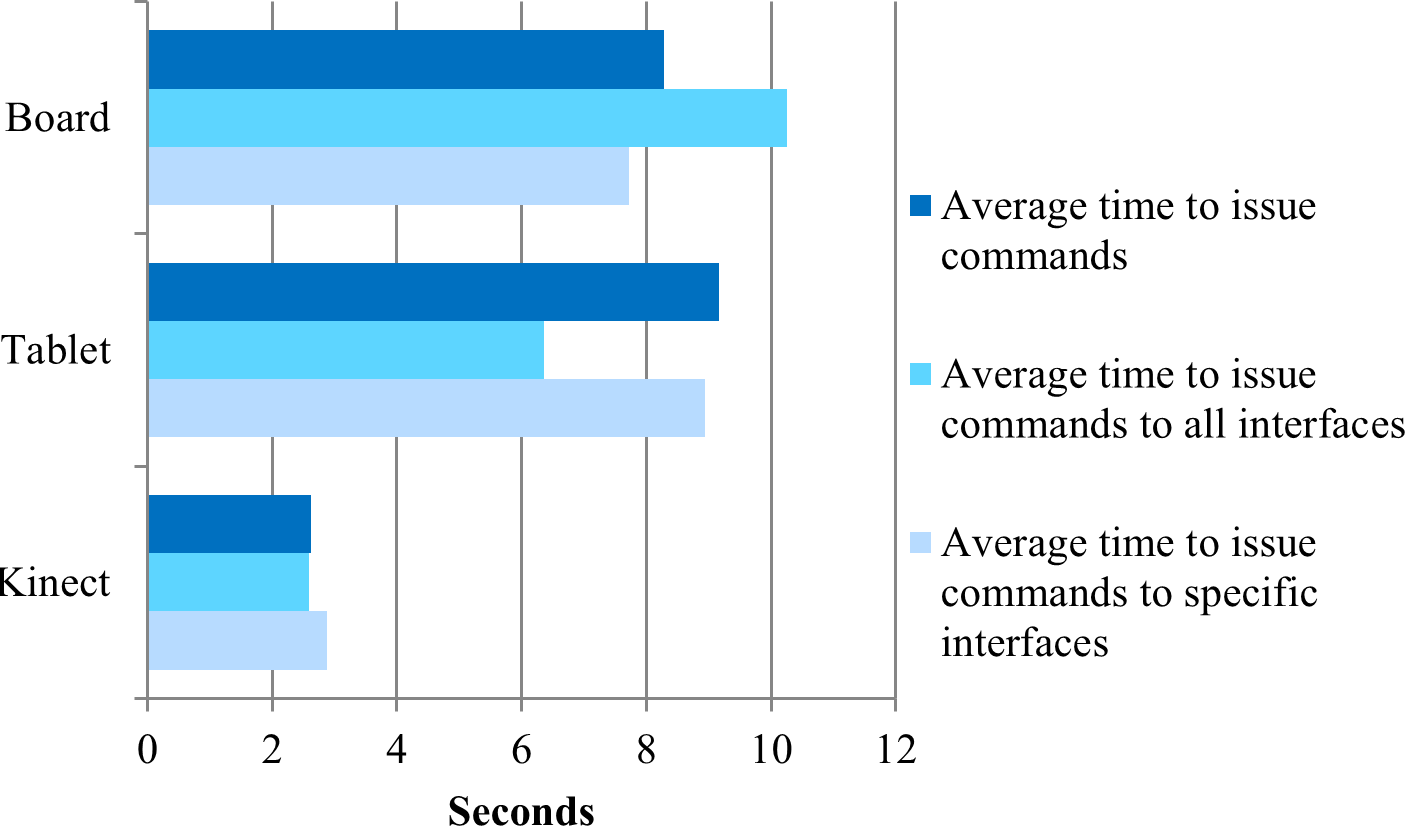
\includegraphics[width=0.45\textwidth]{figures/bar_chart_times.png}
  \caption{Comparison between the times taken to issue commands with each of the control technologies.}
  \label{fig:controlDevicesTimes}
\end{figure}

Figure~\ref{fig:controlDevicesTimes} demonstrates that the Kinect was the quickest control technology for issuing commands from.
This applies to commands in general, commands intended for specific interfaces and commands intended for all interfaces.
The time difference between issuing command intended for all interfaces and commands intended for a selection of specific interface was smallest for the Kinect.
This indicates that the Kinect controls allows for a teacher to put less thought into planning a command since the time difference is less of a restraint.

In the post session interview the teacher expressed a preference for the Kinect.
The teacher stated they like the speed and freedom it offered.
However, the teacher did admit that it could also have been the novelty of the device which drove their preference.

85\% of the errors which occurred in the study were attributed to the Kinect devices' losing track of user limbs.
If the issue of the Kinect losing track of joints was resolved, the error rate would be significantly reduced.
If the errors relating to accuracy had not occurred during the study the error rate would have been 8\%.
Because the remaining errors were deemed to be minor because of their minimal negative consequences the system could be considered fit for purpose.
It is apparent that a method of improving the accuracy of the system's joint tracking is required.

In Section~\ref{subsubsec:pilotdiscussionIssues} the possibility of the Kinect device having difficulty tracking fast moving joints was raised.
Winkler et al.~\cite{Winkler2012} briefly discuss this limitation of the device stating that when the PrimeSense framework is employed, as it is within SynergyNet, fast movement can cause instability.
Replacing all gestures which use movement, i.e. those which consist of pose sequences, were replaced with single poses the potential issues caused by this possibility would be resolved.
This could reduce the errors originating from accuracy issues but would require another changing of the gesture set.
Since the gesture set has been changed already any benefits from the original guessablity would be lost.
Repeating the guessability with the requirements for cohesive poses would be the most desirable approach to building a new gesture set.

However, during the study similar issues were observed to occur when the gesture used to issue the freeze command was executed.
Since this gesture (holding two hands in the air) is a single pose it is implied that the loss of tracking is not entirely due to fast moving joints.
Therefore, other improvements to accuracy may be required.
Alternative or improved technologies may be beneficial as long as they adhere to the other criteria relevant to the tracking device; cost, adaptability, un-encumbering nature and responsiveness.
The Primesense~\cite{Wilson2010} depth camera and Oblong's Mezzanine~\cite{kramer2011} are two possible alternatives that may offer a great accuracy.
In addition to these future versions of the Kinect could provide more accurate results.

As an alternative to improving the accuracy of the system with alternative technologies, future work could entail utilising more Kinects.
The improvements to SynergyNet allowed for any number of Kinects to be used with the framework.
However, the issue of interference would not be resolved through perpendicular as it is with the current system set up.
Therefore, at least one of the interference reducing methods discussed in Section~\ref{subsubsec:studyImplementationMultipleKinects} would be required.
The use of more Kinects could reduce the inaccurate area noted to occupy the edges of the Kinects' view through overlapping the inaccurate region on one Kinect with the accurate centre region on another.

The reduction in error rate appears to be the result of the implemented improvements.
However, a threat to the validity of this claim is the day long training session the teacher required.
The teacher in the previous study only had an hour long session.
The longer training session may have prevented errors which would have still occurred with the improvements.
Future research should entail using teachers with various amounts of training to gauge its influence on the error rate.
Ideally the system should be proved to need a minimal amount of training or else its use could be considered unintuitive.

The accuracy of the Kinect devices resulted in the system being made unfit for purpose.
If this issue was resolved the system would be a viable classroom technology control system.
Issues outlined in this work could be present in any open-air gesture system.
The improvements implemented into SynergyNet were shown to be successful where the accuracy of the Kinects was not concerned.
Therefore, these improvements can be considered suitable for any other open-air gesture system which could potentially suffer from the same issues.

\begin{ack}

This work was partially funded under the UK's EPSRC/ERSC Teaching and Learning Research Programme (TLRP) {\emph{SynergyNet}} project (RES-139-25-0400).
The authors would also like to thank the members of the Durham University Technology Enhanced Learning Special Interest Group for supporting the redrafting of this manuscript, specifically Andrew Joyce-Gibbons.
The source code for the software implemented in the studies discussed in this manuscript is freely available here: \url{https://github.com/synergynet/synergynet3.1}.

\end{ack}

\makeatletter
\def\@biblabel#1{}
\makeatother

% Bibliography
\bibliographystyle{apa}
\bibliography{kinectpaper}

\end{document}
